%% LyX 1.6.5 created this file.  For more info, see http://www.lyx.org/.
%% Do not edit unless you really know what you are doing.
\documentclass[english]{article}
\usepackage[T1]{fontenc}
\usepackage[latin9]{inputenc}
\usepackage[letterpaper]{geometry}
\geometry{verbose,tmargin=1in,bmargin=1in,lmargin=1in,rmargin=1in}
\usepackage{amstext}
\usepackage[authoryear]{natbib}
\usepackage{graphicx}
\usepackage[figurename=Figure]{caption}
\usepackage{subcaption}
\usepackage{grffile}

%%for non-italic greek letters
\usepackage{upgreek}
\usepackage{textgreek}

%% for multirow tables
\usepackage{multirow}

%% for links
\usepackage{hyperref}
\hypersetup{
	colorlinks=true,
	urlcolor=blue, 
	citecolor=blue,
	linkcolor=blue
}

%% for cross referencing. Must be loaded after hyperref (For some reason)
\usepackage[capitalise, noabbrev]{cleveref}

\graphicspath{LIMMA09_2018}
%%%%%%%%%%%%%%%%%%%%%%%%%%%%%%
%% New commands
\newcommand{\tgf}{TGF-$\upbeta$}
\newcommand{\sma}{$\upalpha$-SMA}

\makeatletter
%%%%%%%%%%%%%%%%%%%%%%%%%%%%%% Textclass specific LaTeX commands.
\newcommand{\lyxaddress}[1]{
\par {\raggedright #1
\vspace{1.4em}
\noindent\par}
}
\newenvironment{lyxlist}[1]
{\begin{list}{}
{\settowidth{\labelwidth}{#1}
 \setlength{\leftmargin}{\labelwidth}
 \addtolength{\leftmargin}{\labelsep}
 \renewcommand{\makelabel}[1]{##1\hfil}}}
{\end{list}}

\makeatother

\usepackage{babel}

\begin{document}
\title{Temperol dynamics of gene activity in neonatal, senescent and adult dermal fibroblasts in response to \tgf{}}

%Exploring temperol differences between gene activity of neonatal, senescent and adult dermal fibroblasts by high throughput qPCR and mechanistic modelling

\author{John Smith$^{\text{}1}$, Joann Smith$^{\text{}2}$, Peter Parker$^{\text{}2}$,
Lois Lane$^{\text{}3,*}$}

\maketitle

\lyxaddress{1. Address and Affiliation.\\
2. Address and Affiliation.\\
3. Address and Affiliation.}


\lyxaddress{{*} Corresponding Author: Lois Lane, contact information.}
\begin{lyxlist}{00.00.0000}
\item [{Subject~categories:}] Cell Cycle, Bioinformatics, Proteins
\item [{Keywords:}] template, sample, latex
\item [{Running~Title:}] EMBO/MSB latex template
\item [{character~count~(including~spaces):}] ?
\end{lyxlist}
\newpage{}

%
\section*{Abstract}
Skin is a complex and heterogeneous tissue where both epidermal and dermal skin compartments constantly undergo turnover, remodelling their structure in response to biochemical cues such as \tgf{}. With age, the composition of skin is compromised rendering aged tissue less able to perform its functions. There are some known differences between old and young dermis but a more complete understanding would help us in efforts to restore function. In this study we have performed a high throughput qPCR experiment to measure the dynamics of 72 transcripts that either encode ECM or \tgf{} signalling proteins. The experiment was performed with and without \tgf{} stimulation for 12 time points over 96h in 3 cell lines apiece for neonatal, irradiation-induced senescent and adult cell lines. Our results show that clear differences exist in the dynamics of the selected genes when comparing the different cell lines. Moreover, our statistical analysis provides an indication of which genes are different between groups. The data collected in this experiment is presented as a web application designed for interactively exploring this dataset (\url{http://cwelsh2.pythonanywhere.com}). Collectively this work furthers our understanding of how age and senescence affects the dermis which is an essential step that precludes the understanding of why differences exist and how to rectify them.

%Finally, a small selection of the data has been used to inform a mechanistic model that proposes connective tissue growth factor (CTGF) dynamics as critical in \tgf{}-induced collagen production
%\paragraph*{This should be a single paragraph not exceeding 175 words. The Abstract
%Ageing predisposes individuals to disease
%should be comprehensible to readers before they have read the paper,
%and abbreviations should be avoided. Reference citations within the
%abstract are not permitted.}

\newpage{}


\section*{Introduction}
%emphasise what is known about differences between adult and neonatal fibroblasts - and senescent
Ageing can broadly be described as the progressive deterioration of biological function with time. While not itself a disease, ageing is the biggest risk factor for neurodegenerative, cardiovascular and cancerous diseases \citep{Niccoli2012}. With an increasingly ageing population it is important to study how tissues age to better understand how we might develop the therapeutic potential to promote healthy ageing. %\citep{Jaul2017}. 

Skin is the largest organ in the human body. Beyond the barrier function, skin is involved in sensory perception, thermoregulation and immunosurveillance \citep{Farage2009}. Like other tissues, skin is subject to intrinsic ageing and the ability of skin to perform these functions becomes diminished. Phenotypically, old sky is dry, rough and itchy with uneven pigmentation, a reduced capacity for wound healing, wrinkles and collagen and elastin networks that are impaired by reductions and fragmentation. Old skin has diminished hair growth and sebaceous gland function, flatter dermal papillae, reduced melanocyte concentrations and less cellular turnover, compared with young skin. The ageing of skin is the most visible aspect of ageing in general and the resulting phenotypic changes in its structure and appearance have an important impact both on physiological and psychological well-being \citep{Blume-Peytavi2016, Farage2009}. A greater understanding of how skin ageing manifests would benefit the development of therapeutic and cosmetic interventions to promote healthy skin ageing. 

Skin is a multi-layered tissue composed of an outer epidermis and a underlying dermis. The epidermis is comprised mainly of keratinocytes which are avascular and gradually differentiate and harden as they progress outwards towards the skin surface. Beneath the epidermis lies the dermal-epidermal junction which is a thin basement membrane that enables communication between the dermis and epidermis. The dermis is a vascular, cellular sparse tissue composed mostly of a fibrous connective tissue known as the extracellular matrix (ECM). Dermal tissue is essential for skin integrity and provides structural and nourishing support for the epidermis \citep{Lu2011}. 

Much like other tissues, an essential aspect of dermal ECM biology is that function arises as a consequence of structure. Dermal fibroblasts are responsible for synthesising ECM components (Ref) as well as those which degrade the ECM (ref). Fibroblasts respond to biochemical cues such as stimulation by transforming growth factor $\upbeta$ (\tgf{}) or TNF-$\upalpha$ which induces changes to the fibroblast metabolic output. In age, the composition of the dermal microenvironment is different from young tissue. Young skin is optimized to perform its functions but with age, the composition of skin changes rendering less able to perform its function. 

The biochemical changes that occur in the aged dermis are global and incompletely defined. One of the best understood differences is that type 1 collagen, the most abundant protein in the dermis, is reduced in numbers. This is thought to arise from both reduced production by fibroblasts and increased degradation by matrix metalloproteinases (MMPs) (\cite{Fisher2009}). Collagen fibrils also become increasingly fragmented with age which contributes to the ageing phenotype \citep{Quan2015, Fisher2009, Varani2006}. Moreover, other biochemical mediators such as \tgf{} or connective tissue growth factor (CTGF) that have an overall pro-anabolic effect in the dermis are produced to a lesser degree and have modified intracellular biochemistry for signal transduction \citep{Quan2010}. The aged dermal environment contains higher levels of MMP1 which contribute towards the degradation and damage of collagen networks \citep{Fisher2009}. 

The aged dermal environment contains an increasing population of senescent dermal fibroblasts. Cells have a limited replicative potential (ref) and when they can no longer proliferate they undergo replicative senescence. Importantly, senescent cells remain metabolically active and can interfere with normal physiology by secreting proteins into the ECM \citep{Toutfaire2017}. The collective profile of proteins that are secreted are known as the age-associated secretory profile or SASP (ref). 

\tgf{} signalling is essential for ECM homeostasis because it controls the production of many ECM components including type 1 collagen, fibronectin, elastin and others (ref). Moreover, in age there are alterations in the \tgf{} network that contribute towards the ageing phenotype. Notably, loss of Smad3 in aged fibroblasts has been proposed as a mechanism of reduced collagen levels \citep{Purohit2016}.

In this study, we have conducted a high throughout qPCR experiment designed to study the transcriptional differences between neonatal, adult and irradiation-induced senescent fibroblasts. Fibroblasts were treated with \tgf{} or a negative control over time to compare the dynamics of gene activity between cell lines. We discuss some of these differences and provide an interactive web interface into the data for readers to explore the dataset. 

\begin{figure}
	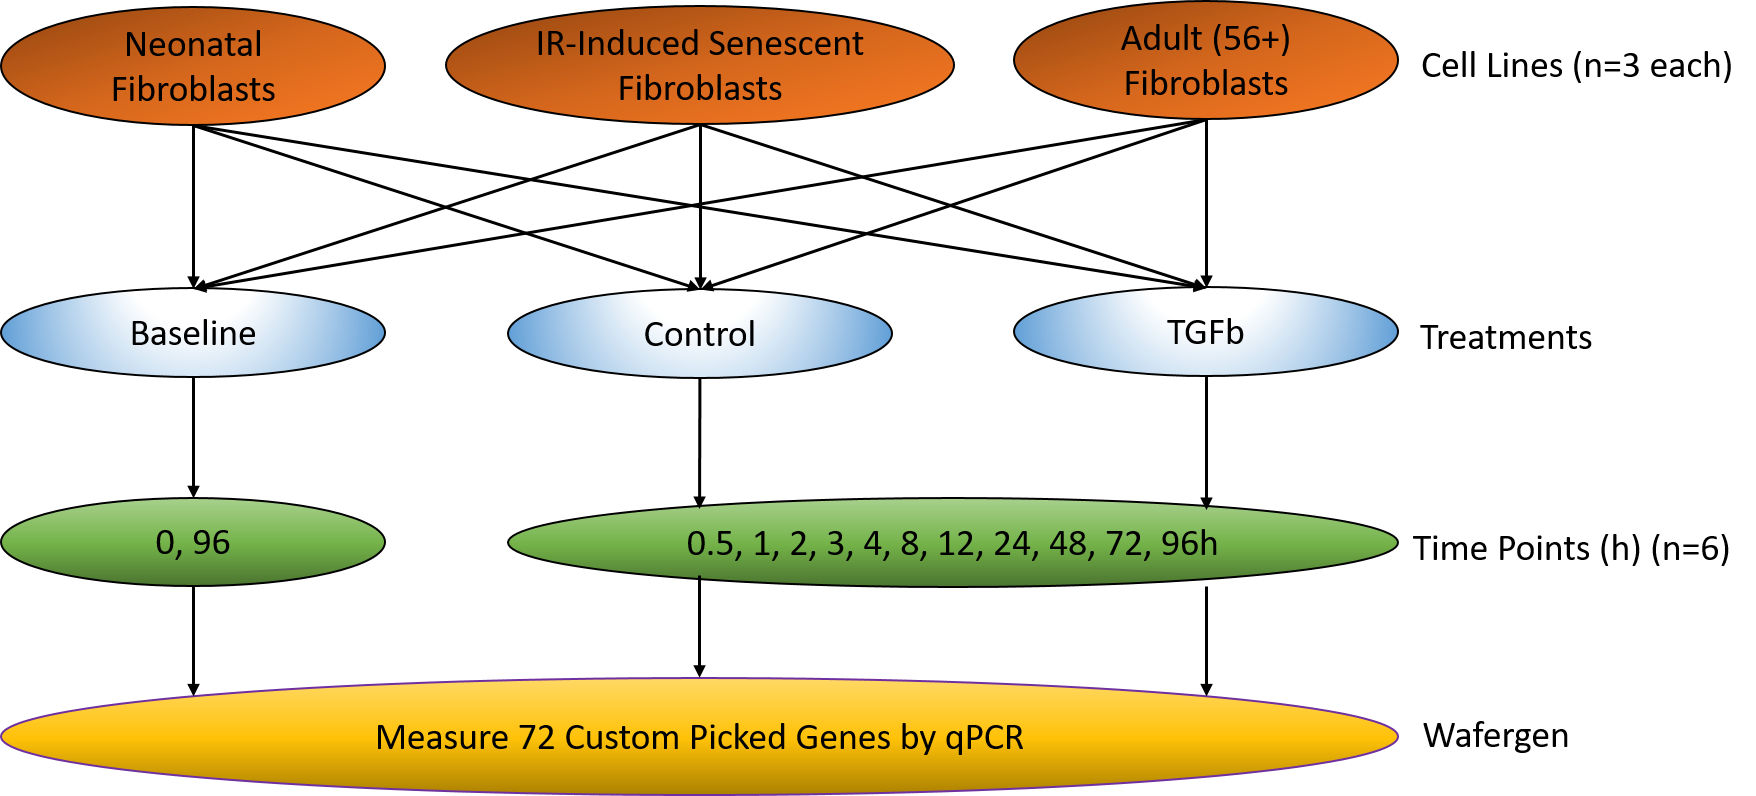
\includegraphics[width=\textwidth]{img/ExperimentDesign}
	\caption{Graphical depiction of experimental design}
	\label{fig:exp_design}
\end{figure}
\section*{Results}
%\subsection{Temperol gene expression dynamics in neonatal, adult and senescent cell lines in response to \tgf{}}
%\subsubsection{Experiment design}
To identify some of the differences between neonatal, irradiation-induced senescent and adult fibroblasts, the activity of 72 genes was measured over 96h in 3 replicates of each cell group using high throughput qPCR. These measurements were taken both in response to 5ng mL$^{-1}$ \tgf{} reconstituted in 10mM citric acid or 0.1\% BSA in 10mM citric acid as a negative control. The genes measured were manually selected based on a literature search to be relevant to ECM biology or \tgf{} signalling. The design of this experiment is depicted in (\cref{fig:exp_design}).

\begin{figure}[t]
	\centering
	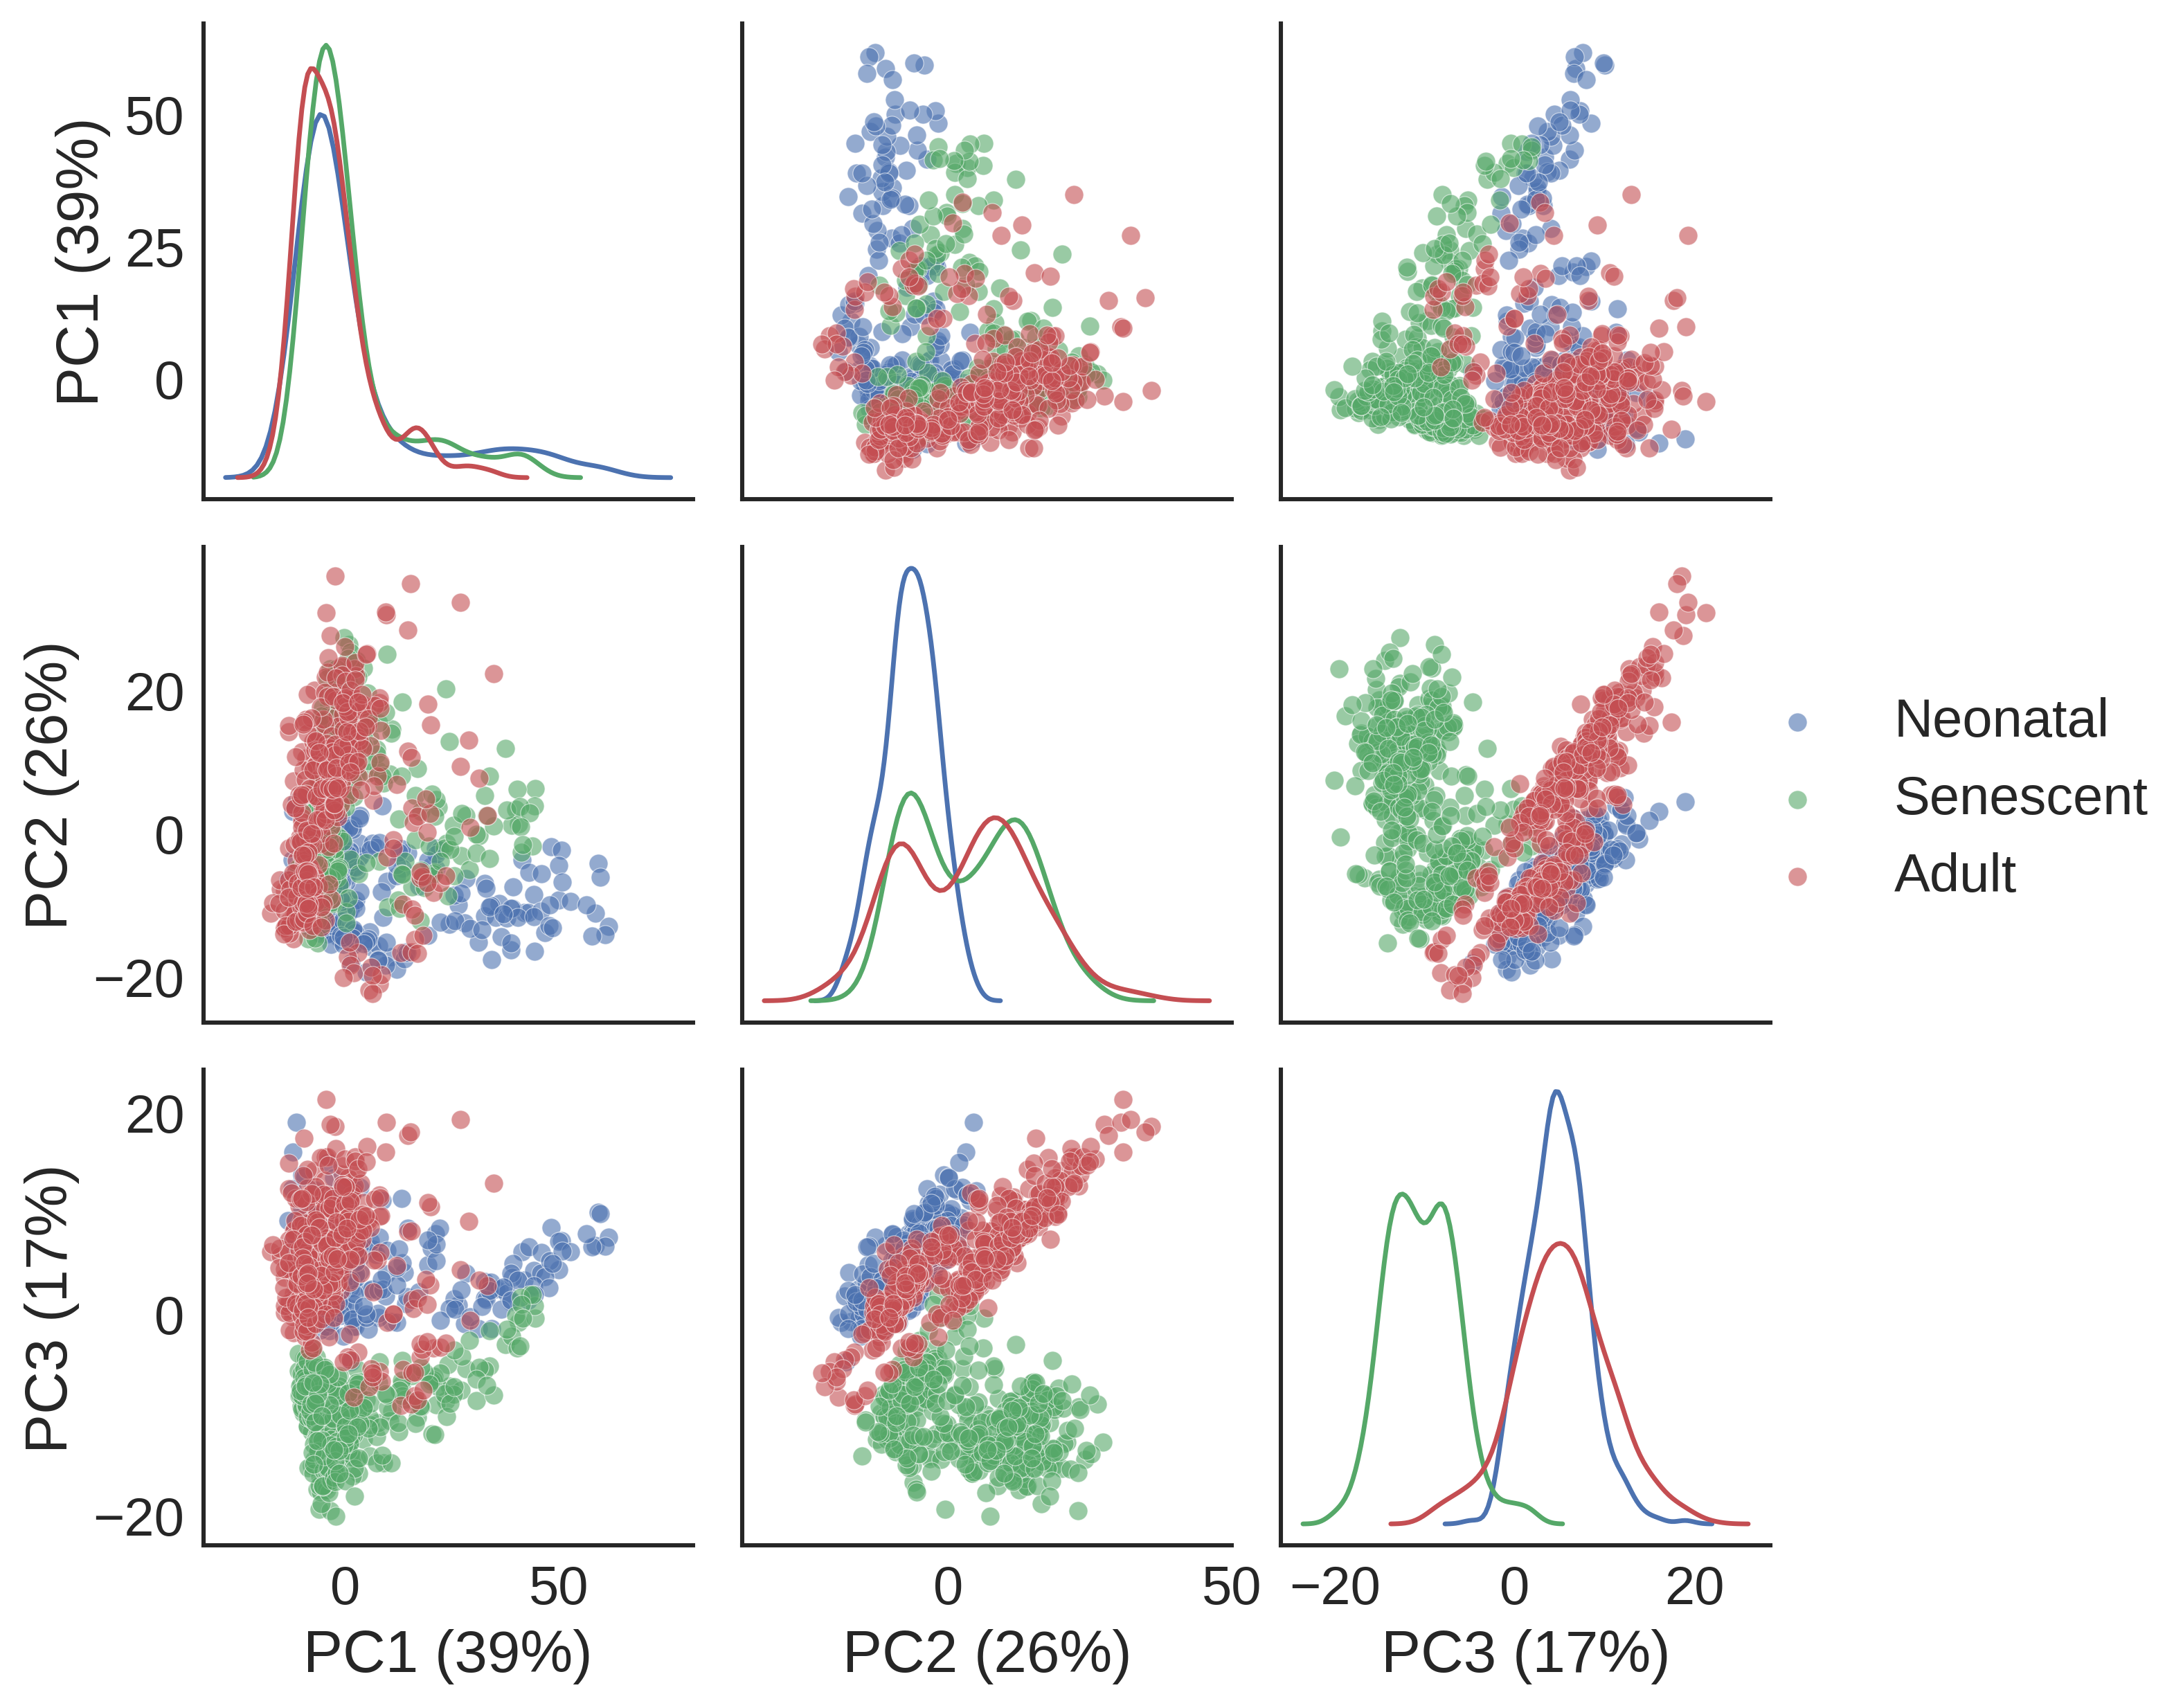
\includegraphics[width=\textwidth]{img/qc/cell_line}
	\caption{Scatter matrix of first three principle components coloured by cell line. Kernel density plots along the diagonal represent the distribution of the relevant principle component.}
	\label{fig:qc:cell_line}
\end{figure}

%\subsubsection{Principle component analysis}
Three out of 72 primers (IL1A, IL1B and FOSB) were either unreliable or undetectable and were excluded from further analysis. As a first step in data analysis a principal component analysis (PCA) was conducted to gain confidence in the measurements. The PCA was produced so that each point on the PCA represents one of the 1296 samples. The closer together points lie on the PCA the more similar they are. Therefore it is possible to both positively and negatively assert whether the cells behave as expected. To highlight these experimental factors the same PCA was plotted 5 times, coloured by different experimental factors, namely by cell line (\cref{fig:qc:cell_line}), cell ID (\cref{fig:qc:cell_id}), time points (\cref{fig:qc:time_point}), treatment (\cref{fig:qc:treatment}) and by biological replicates (\cref{fig:qc:replicate}). Because the PCA coloured by cell lines, cell IDs, time points and treatments all display clustering while biological replicates do not, this PCA indicates that the data collected likely represent the underlying biology well. A scree plot is presented in \cref{fig:qc:scree} and indicates that the first three principal components account for >80\% of variance. 

%\subsubsection{Differential expression}
Following the PCA, a differential expression analysis was conducted to investigate whether each measured gene was statistically different: 1) between in adult or senescent cell lines compared to neonatal cell lines ro 2) within each cell group. The R package LIMMA was used for differential expression analysis. Specifically, because our data is dynamic, LIMMA was configured to evaluate whether two full time series objects were different from each other \citep{Ritchie2015, Smyth2004, Smyth2005}. Since we have data from 3 cell lines per cell line group, a comparison between cell lines G and A is just as valid as cell lines H and A, to compare adult and neonatal cells (for example). To make use of the available data, all combinations of cell line were compared using LIMMA, as explained in \cref{fig:stats:diagram}. A total of 10 differential expression analyses were conducted, 5 each to compare \tgf{} or negative control time series, two of which were between groups comparisons and three within groups comparisons. A gene was considered differentially expressed if the FDR corrected p-value was less than 0.001. Since the between groups comparisons totalled 9 LIMMA analyses per comparison and the within groups comparisons totalled 3, an overview of the differential expression analysis is presented in \cref{table:stats_summary} by counting the number of genes which were differentially expressed in >60\% of LIMMA analyses per comparison. The differential expression analysis is expressed as a percentage in \cref{fig:heatmap} and shows that the comparison between \tgf{} treated adult and neonatal cell lines were the most different of all the comparisons, followed by the comparison within \tgf{} treated adult cell lines. The comparison within control treated neonatal cell lines were the least different. Moreover, in all cases, the \tgf{} time series had more differentially expressed genes than the control time series. 

%1) More genes are differentially expressed in the \tgf{} condition than in the control condition in all comparisons made. 
%
%2) as expected, adult cell lines exhibited more variability than neonatal in both control and tgf treatments
%
\begin{figure}
	\centering
	\begin{subfigure}{0.25\linewidth}
		
\includegraphics[width=\linewidth]{img/stats/between_adult}
		\caption{Adult Vs neonatal}
%		\label{fig:diag:b}
	\end{subfigure}\qquad
	\begin{subfigure}{0.25\linewidth}
		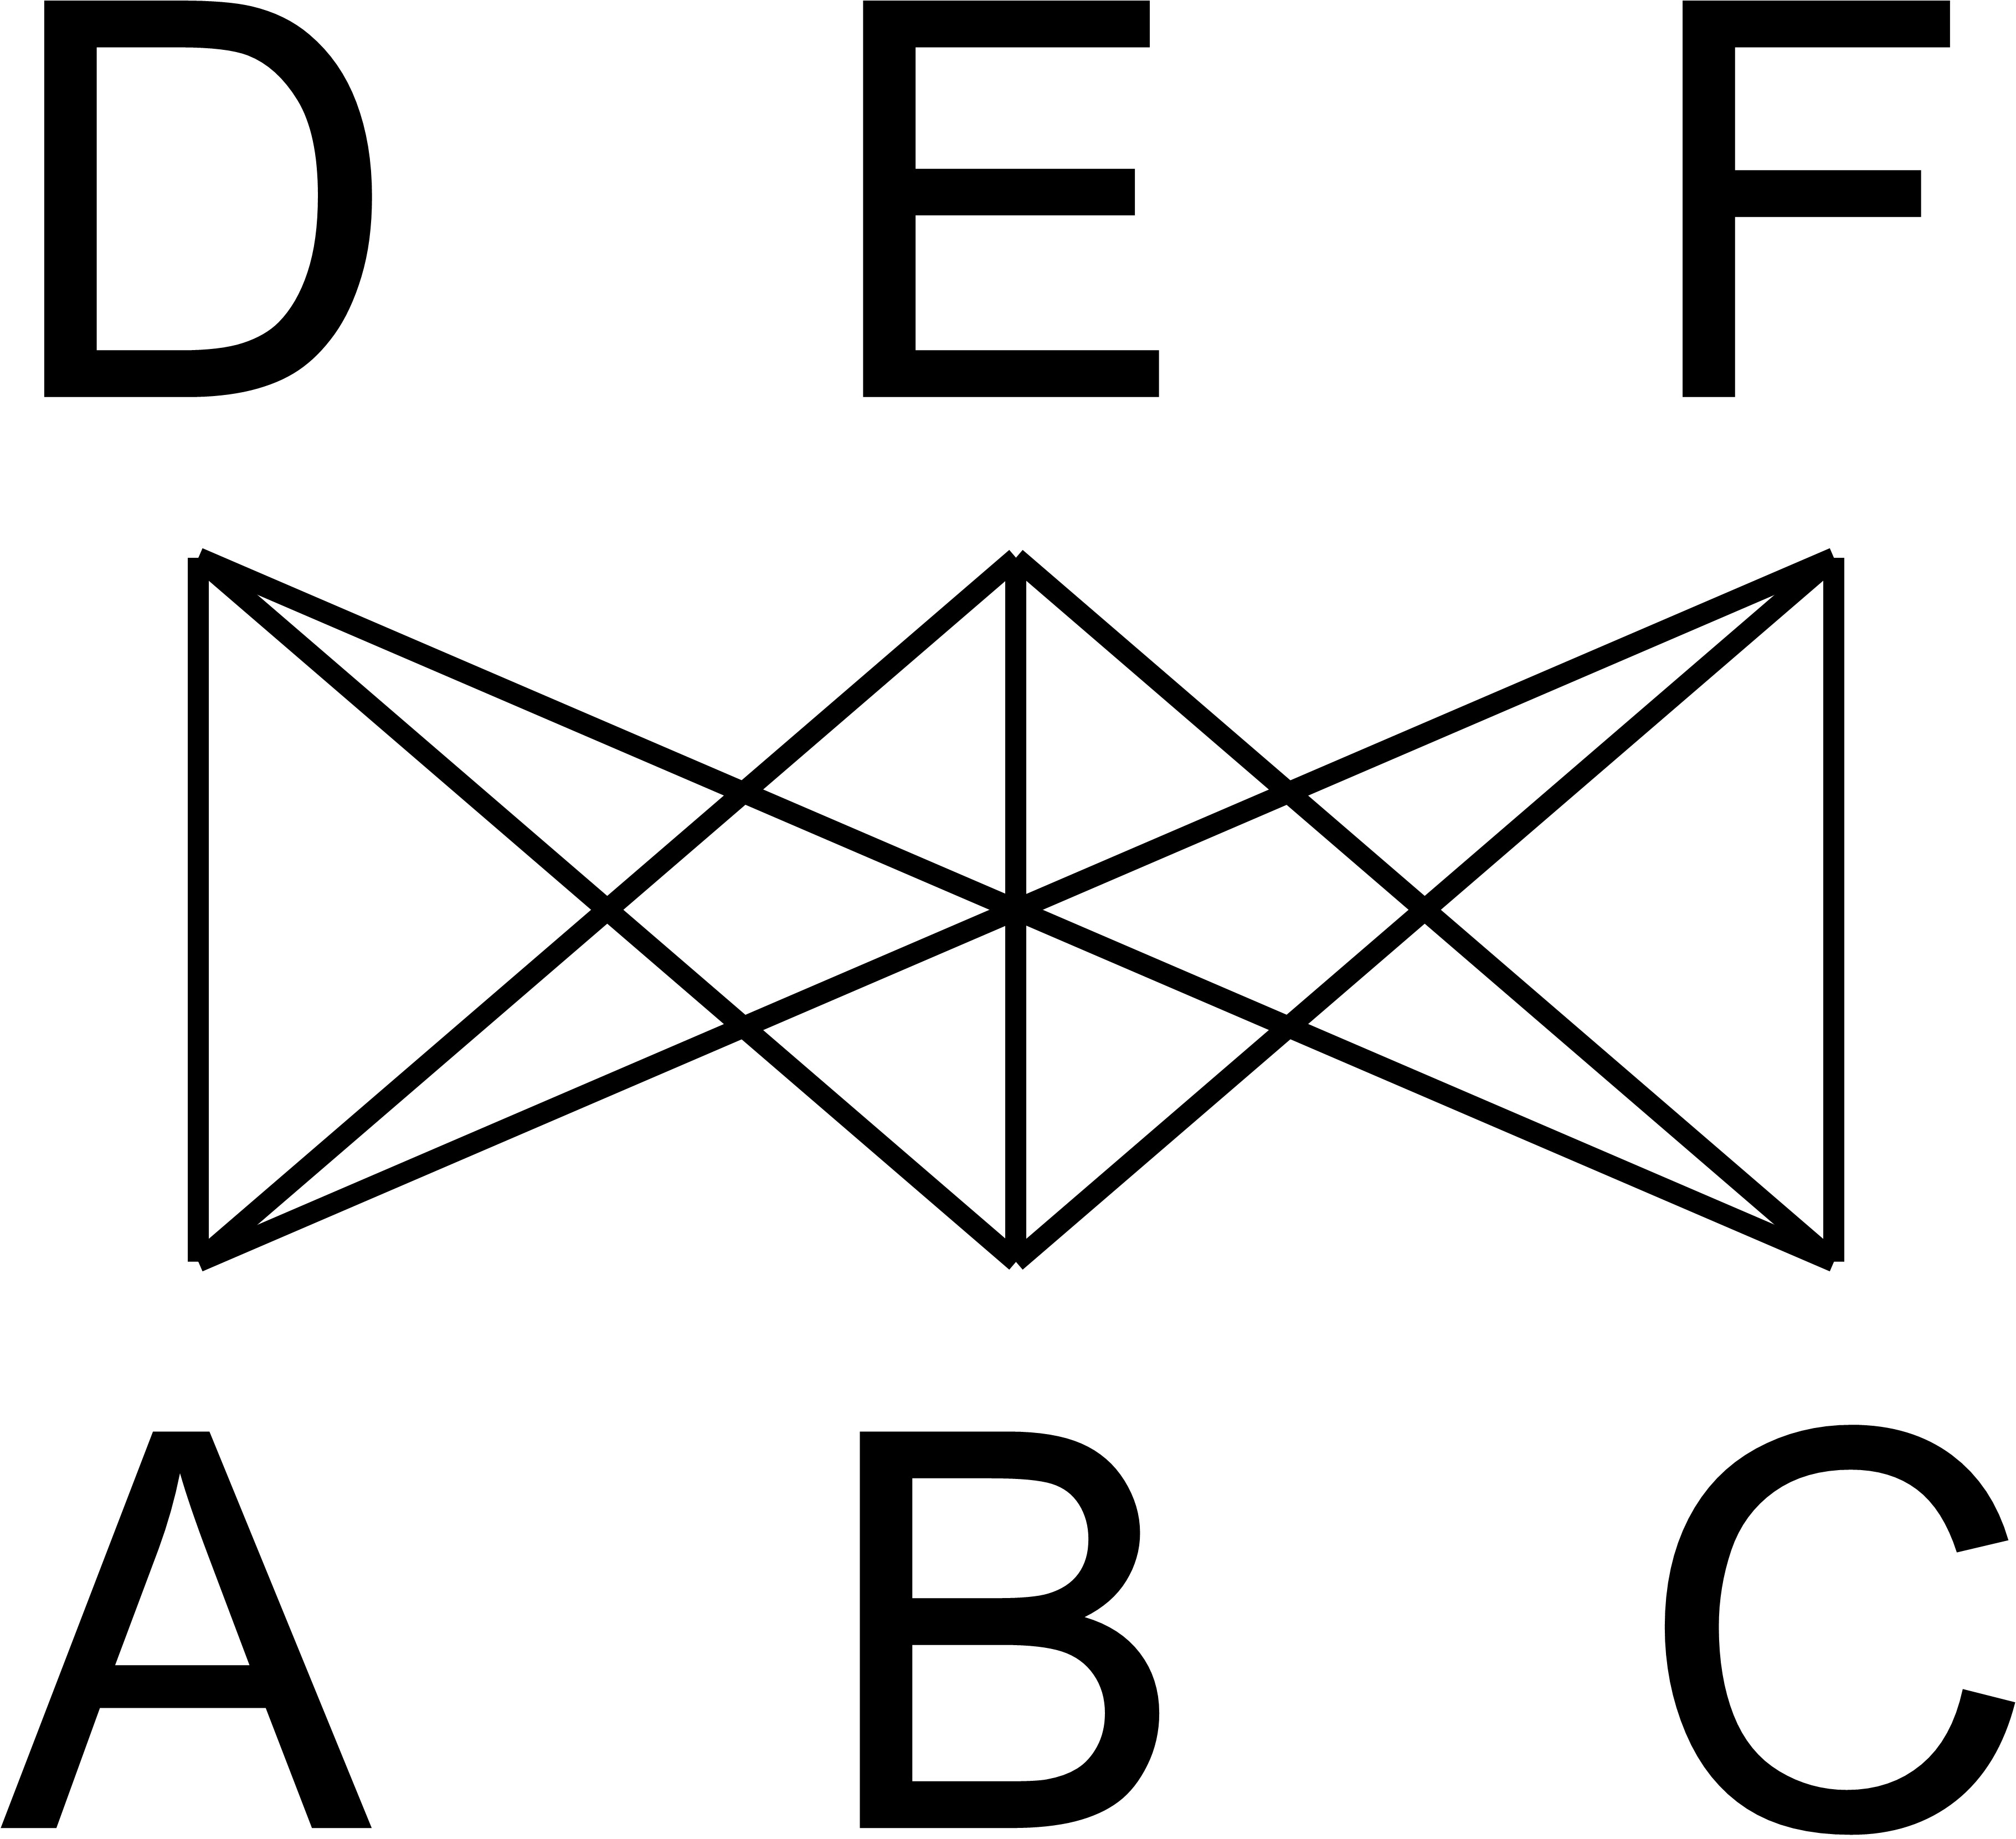
\includegraphics[width=\linewidth]{img/stats/between_sen}
		\caption{Senescent Vs neonatal}
%		\label{key}
	\end{subfigure}

	\begin{subfigure}{0.15\linewidth}
		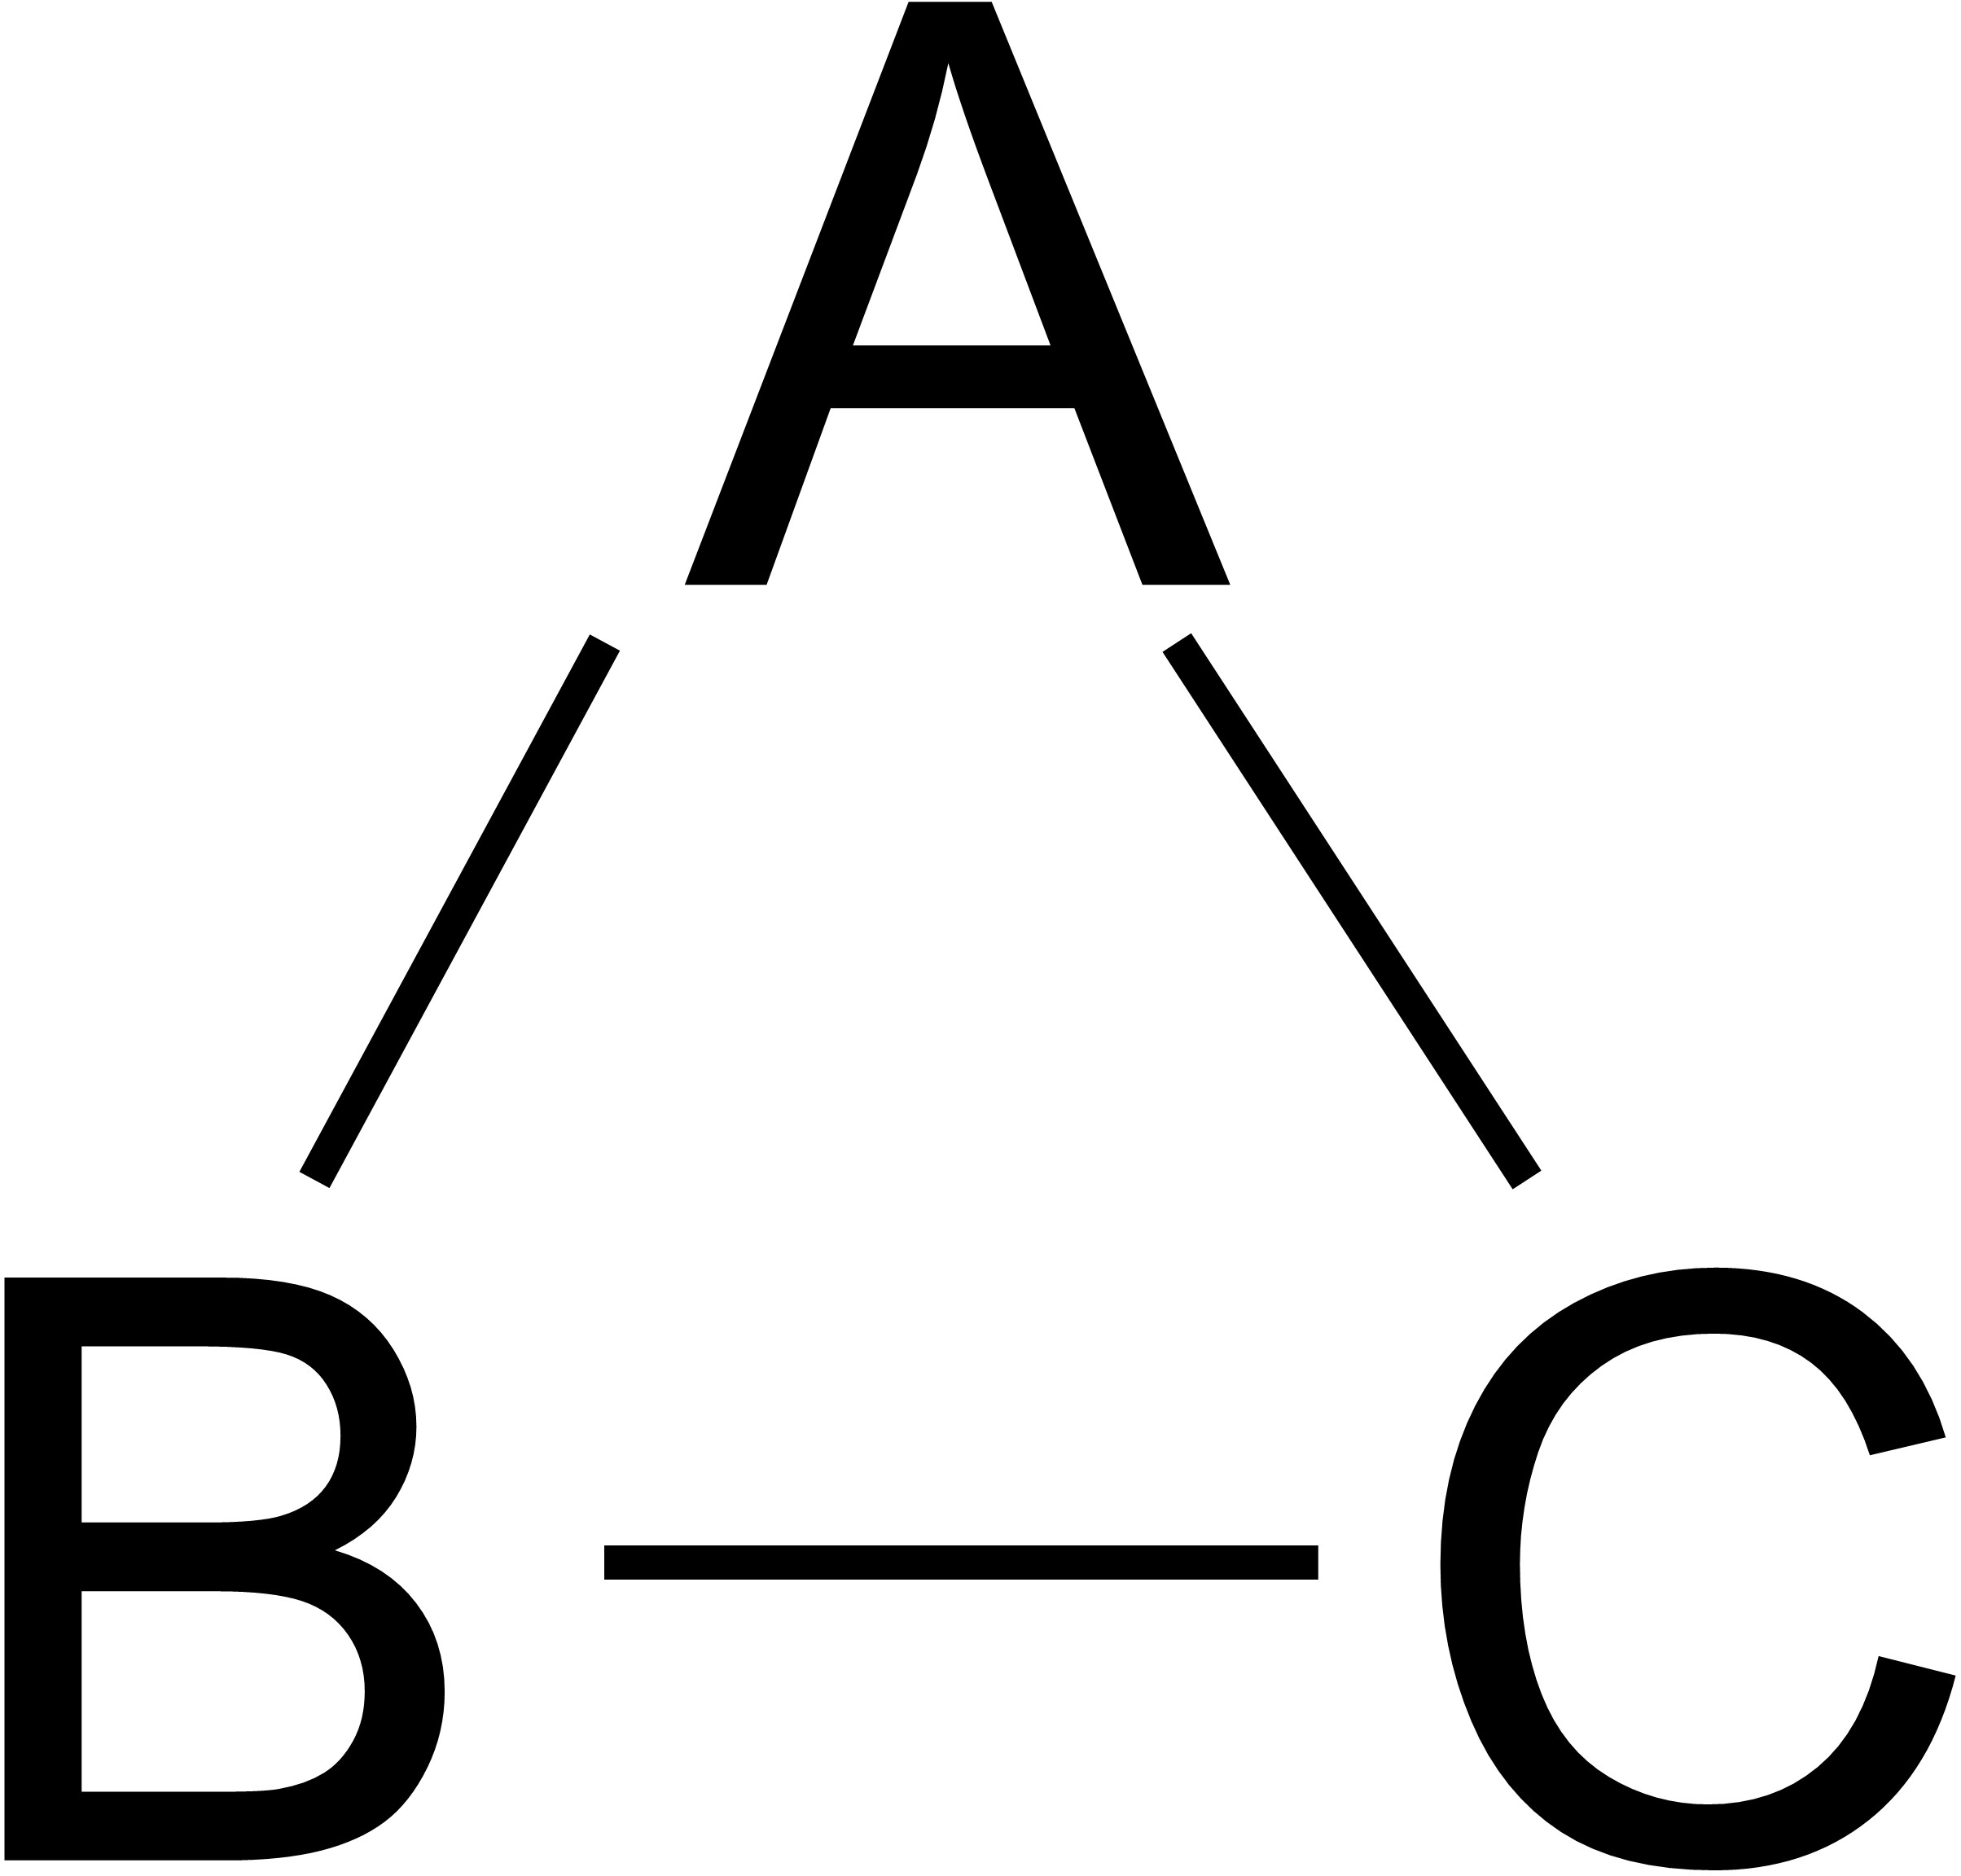
\includegraphics[width=\linewidth]{img/stats/within_neonatal}
		\caption{Neonatal}
%		\label{key}
	\end{subfigure}\qquad
	\begin{subfigure}{0.125\linewidth}
		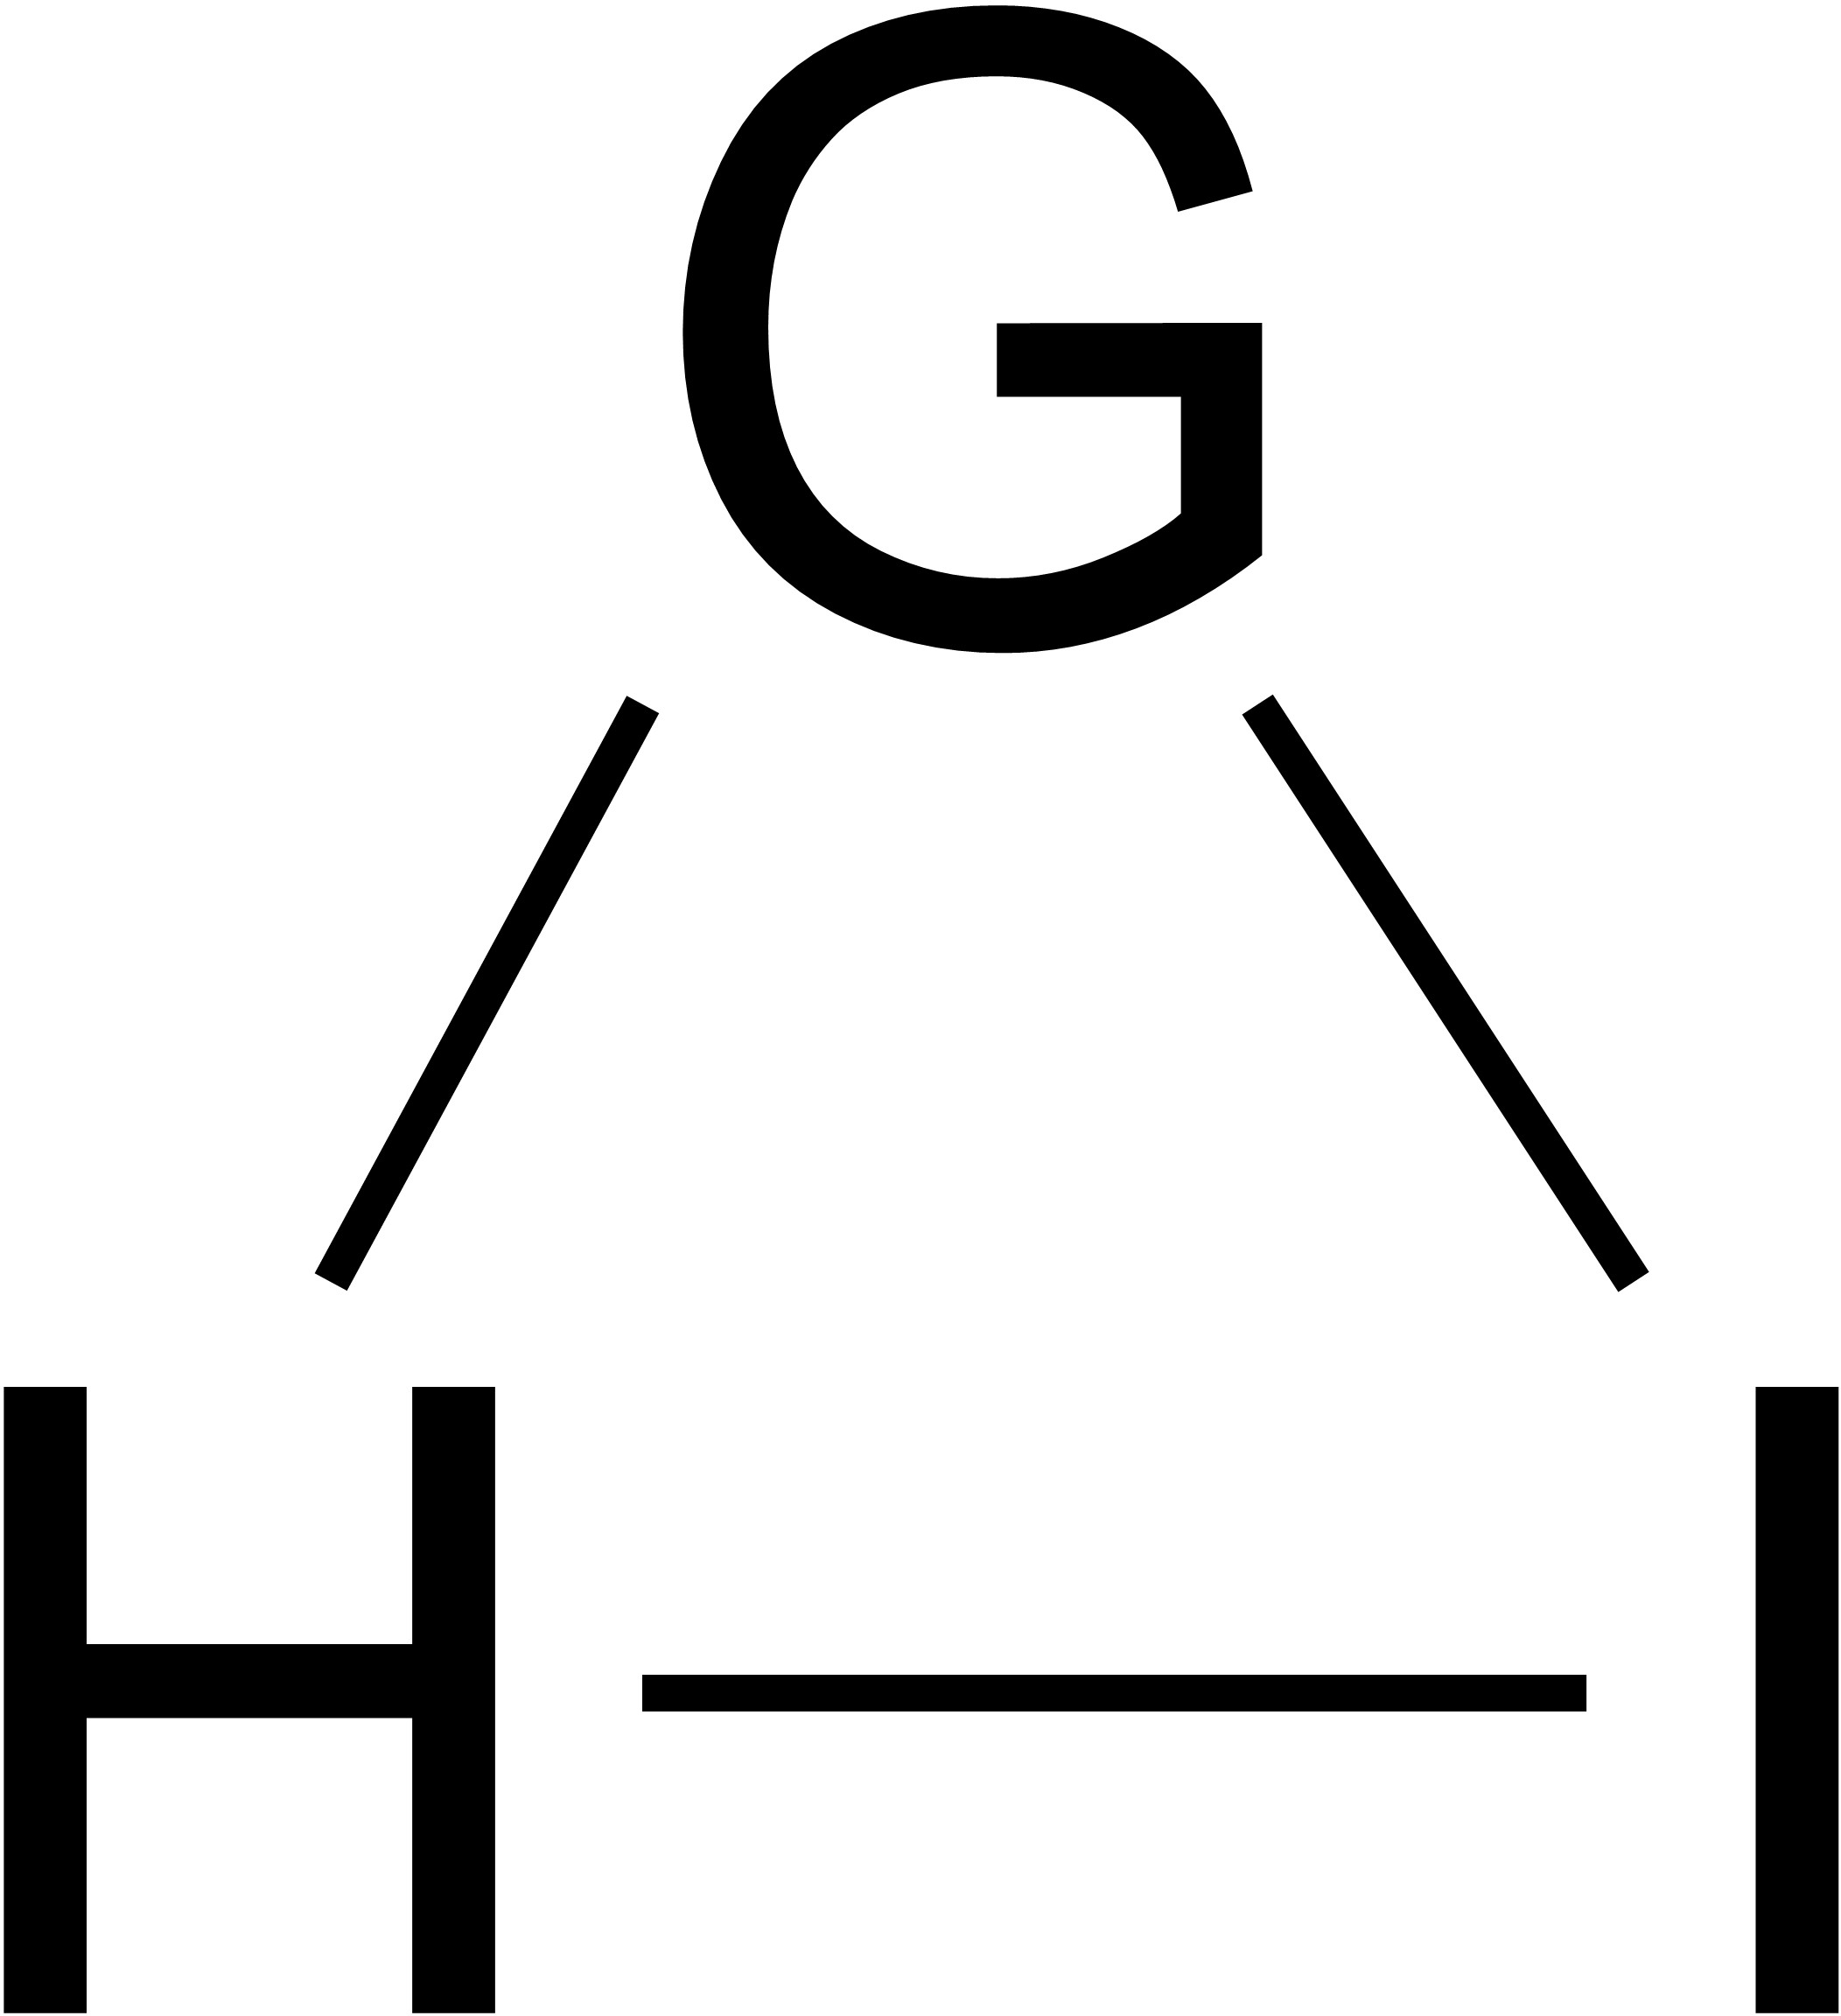
\includegraphics[width=\linewidth]{img/stats/within_adult}
		\caption{Adult}
%		\label{key}
	\end{subfigure}\qquad
	\begin{subfigure}{0.15\linewidth}
		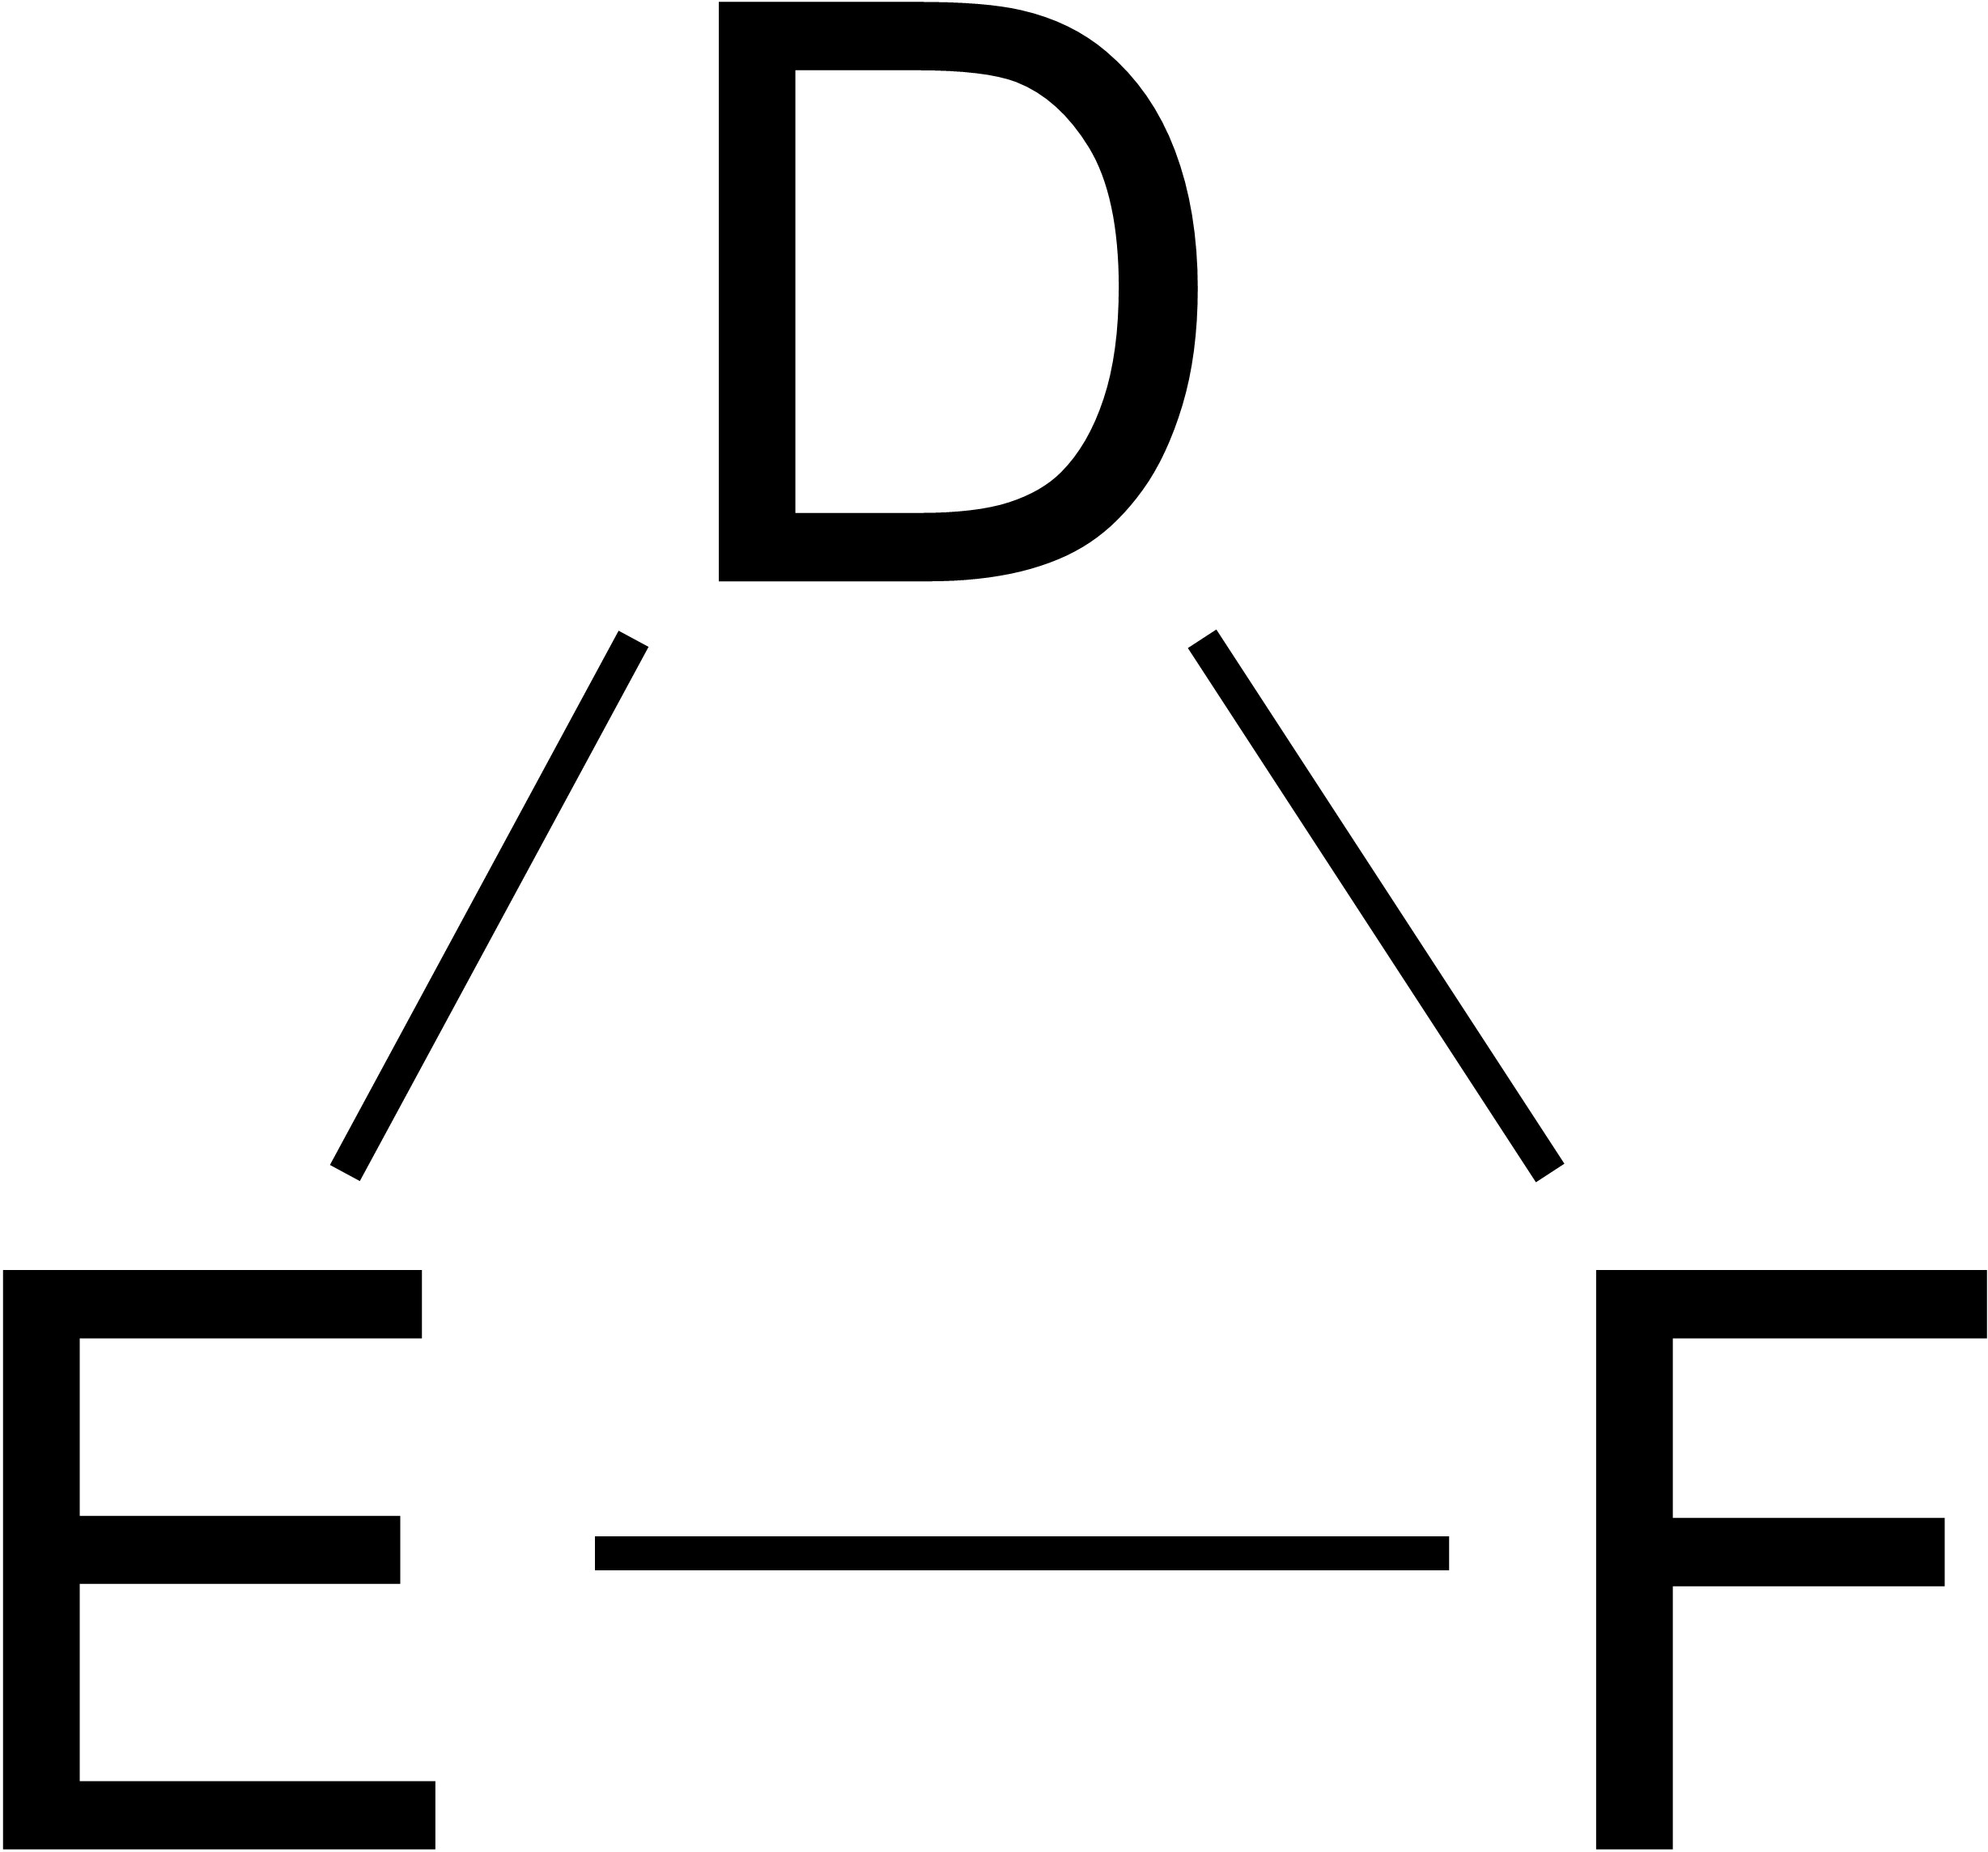
\includegraphics[width=\linewidth]{img/stats/within_senescent}
		\caption{Senescent}
	\end{subfigure}
	\caption{Diagrammatic representation of comparisons made using LIMMA. Letters represent a cell ID while an edge signifies that a LIMMA analysis was conducted between the two. LIMMA analyses were conducted between (a) adult and neonatal and (b) senescent and neonatal. LIMMA analyses were also conducted within (c) neonatal (d) adult and (e) senescent cell lines. All differential expression analyses were conducted using LIMMA's spline method to compare full time series datasets.}
	\label{fig:stats:diagram}
\end{figure}
%
%\begin{table}
%	\centering
%	\caption{Table summarising the number of genes per comparison that were differentially expressed with a (FDR corrected) p-value <0.001 in over 60\% of LIMMA analyses per group.}
%	\begin{tabular}{|l|l|l|}
%		\hline
%		\multirow{2}{*}{\textbf{Comparison}} & \multicolumn{2}{l|}{\textbf{Treatment}} \\ \cline{2-3} 
%		& \textbf{Control} & \textbf{\tgf{}} \\ \hline
%		Adult Vs neonatal & 25 & 51 \\ \hline
%		Senescent Vs neonatal & 21 & 37 \\ \hline
%		Neonatal Vs neonatal & 9 & 33 \\ \hline
%		Adult Vs adult & 24 & 46 \\ \hline
%		Senescent Vs senescent & 17 & 30 \\ \hline
%	\end{tabular}
%	\label{table:stats_summary}
%\end{table}

\begin{figure}
	\begin{subfigure}{0.45\linewidth}
		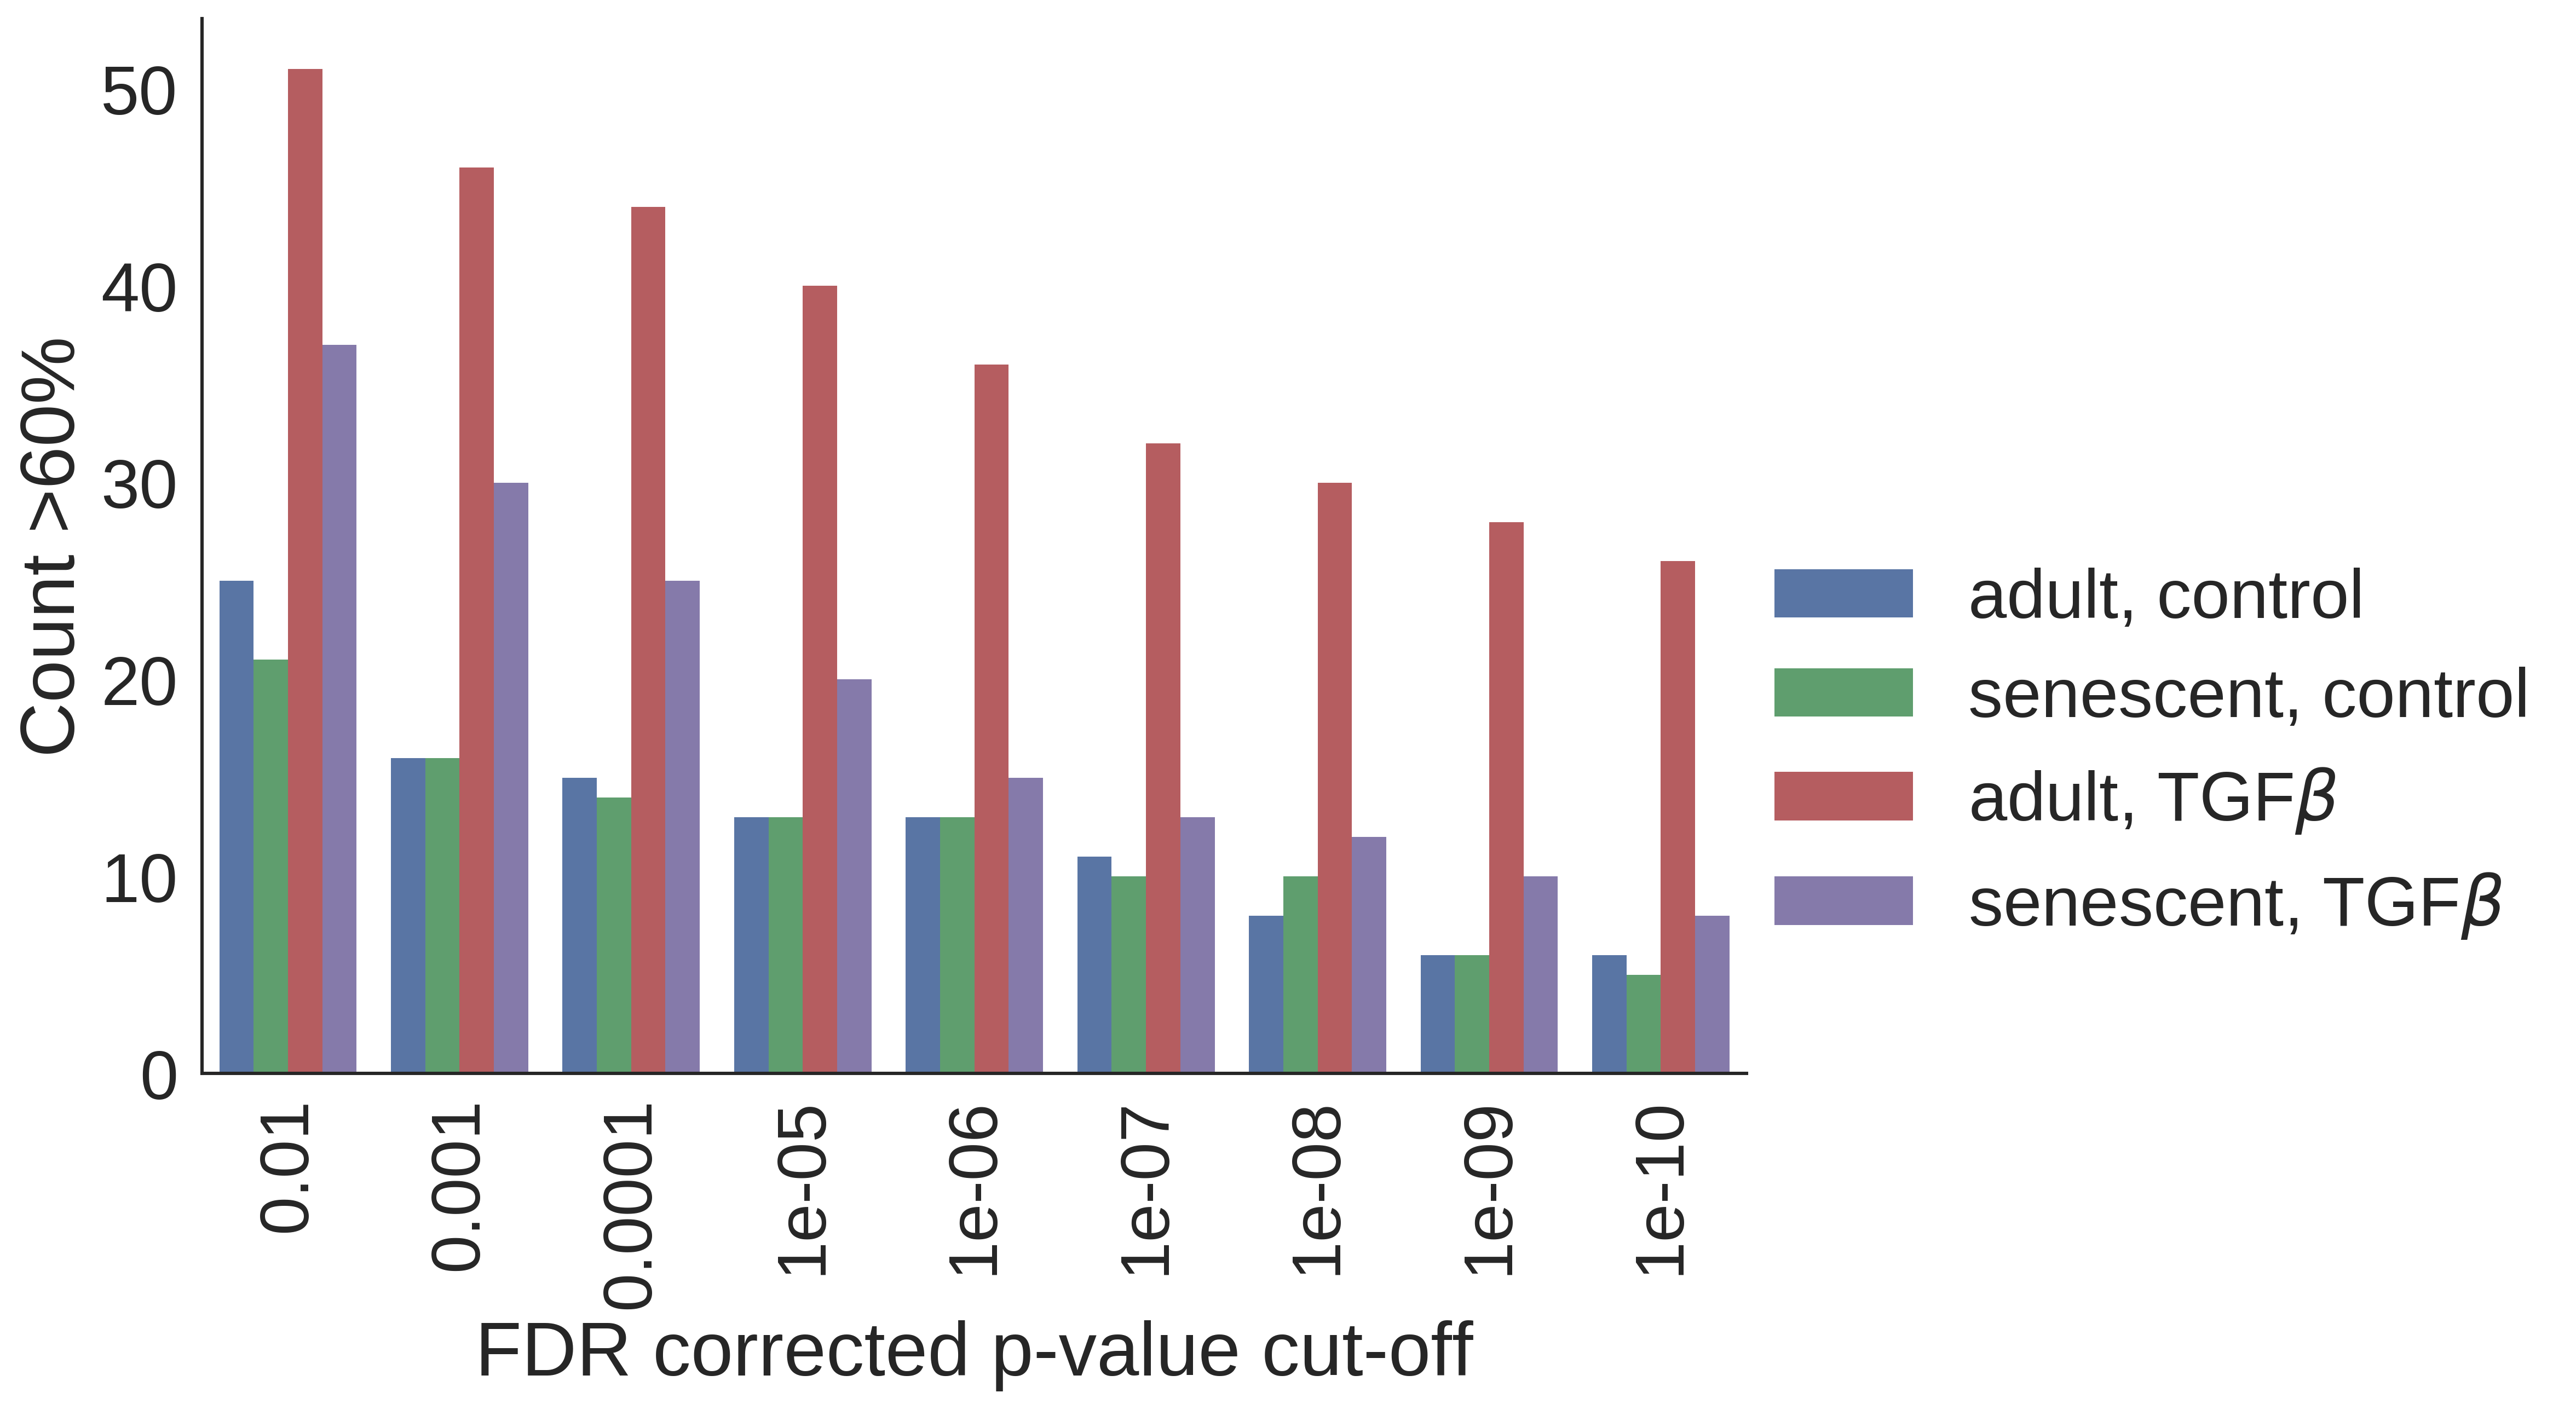
\includegraphics[width=\linewidth]{LIMMA09_2018/SavedObjects/between_pvalue_counts}
		\caption{Between cell lines}
		\label{fig:pvalues:between}
	\end{subfigure}
	\begin{subfigure}{0.45\linewidth}
		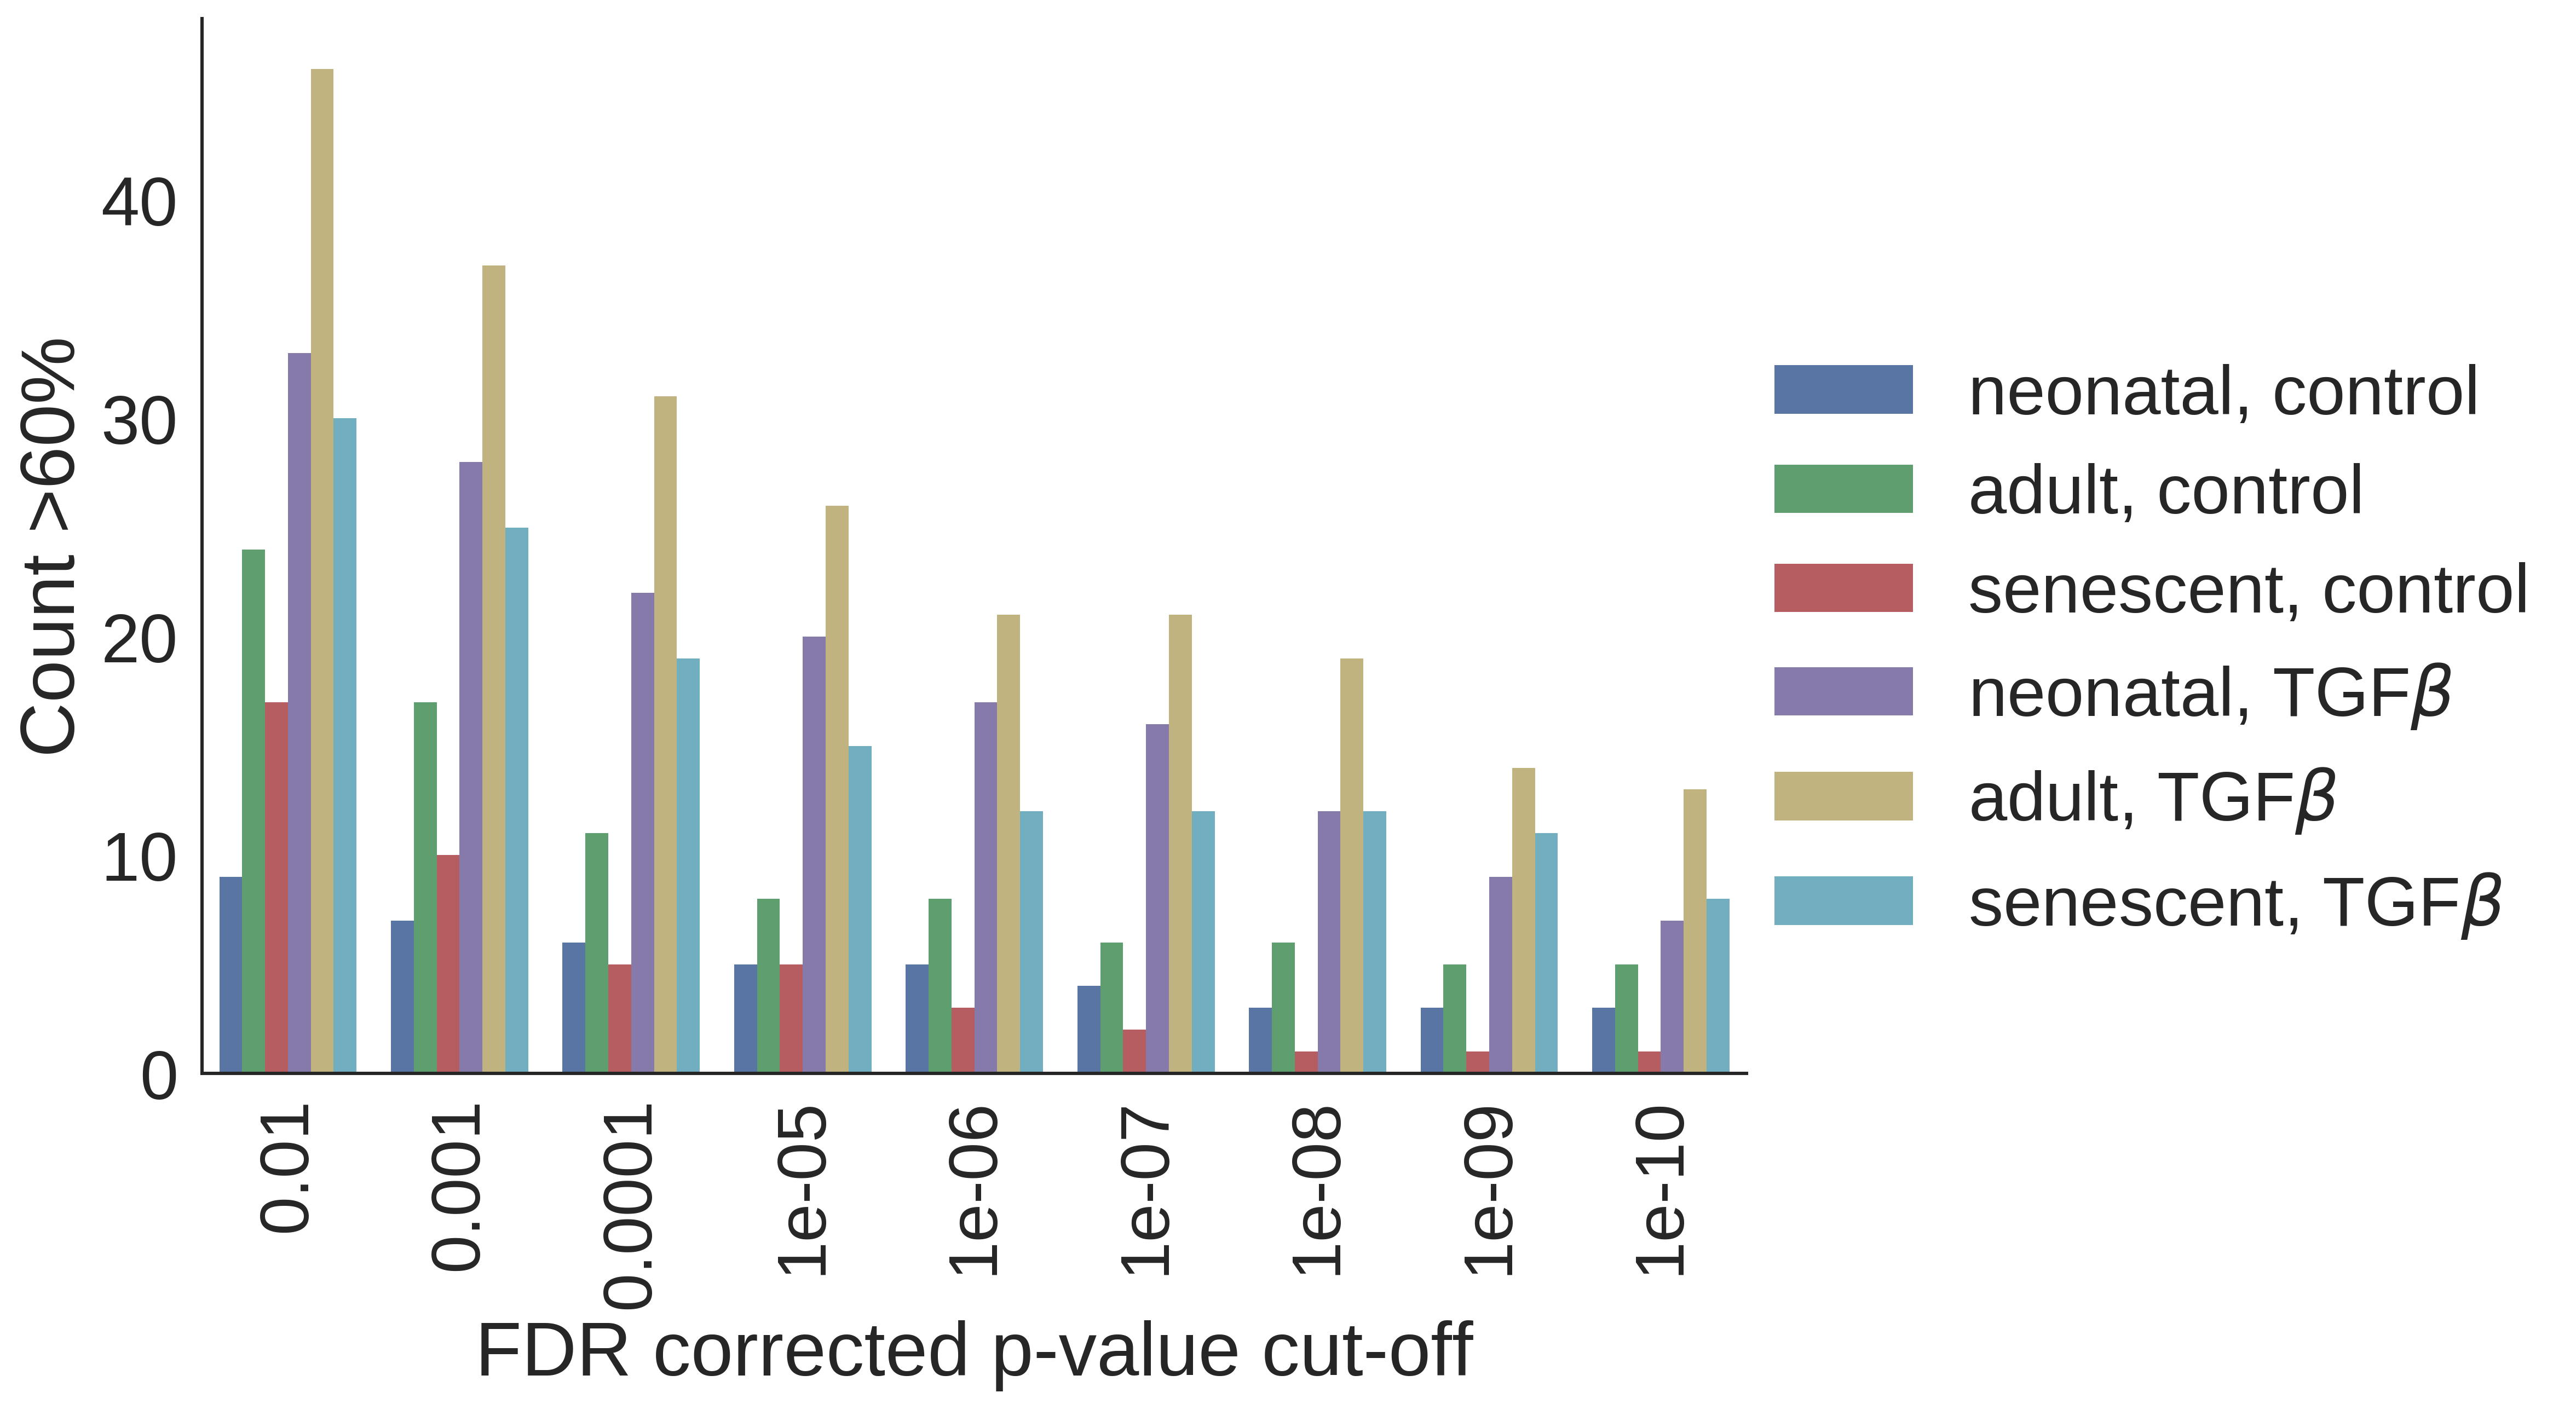
\includegraphics[width=\linewidth]{LIMMA09_2018/SavedObjects/within_pvalue_counts}
		\caption{Within cell lines}
		\label{fig:pvalues:within}
	\end{subfigure}
	\caption{Counts of genes that were differentially expressed in >60\% of LIMMA analyses as a function of p-value for (a) the between groups and (b) within groups comparisons.}
	\label{fig:pvalues}
\end{figure}

\begin{figure}
	\centering%C:\Users\Ciaran\Box Sync\WafergenPaper\LIMMA09_2018\SavedObjects\analysis_at_pval_less_than_0_001
	\begin{subfigure}{0.45\linewidth}
		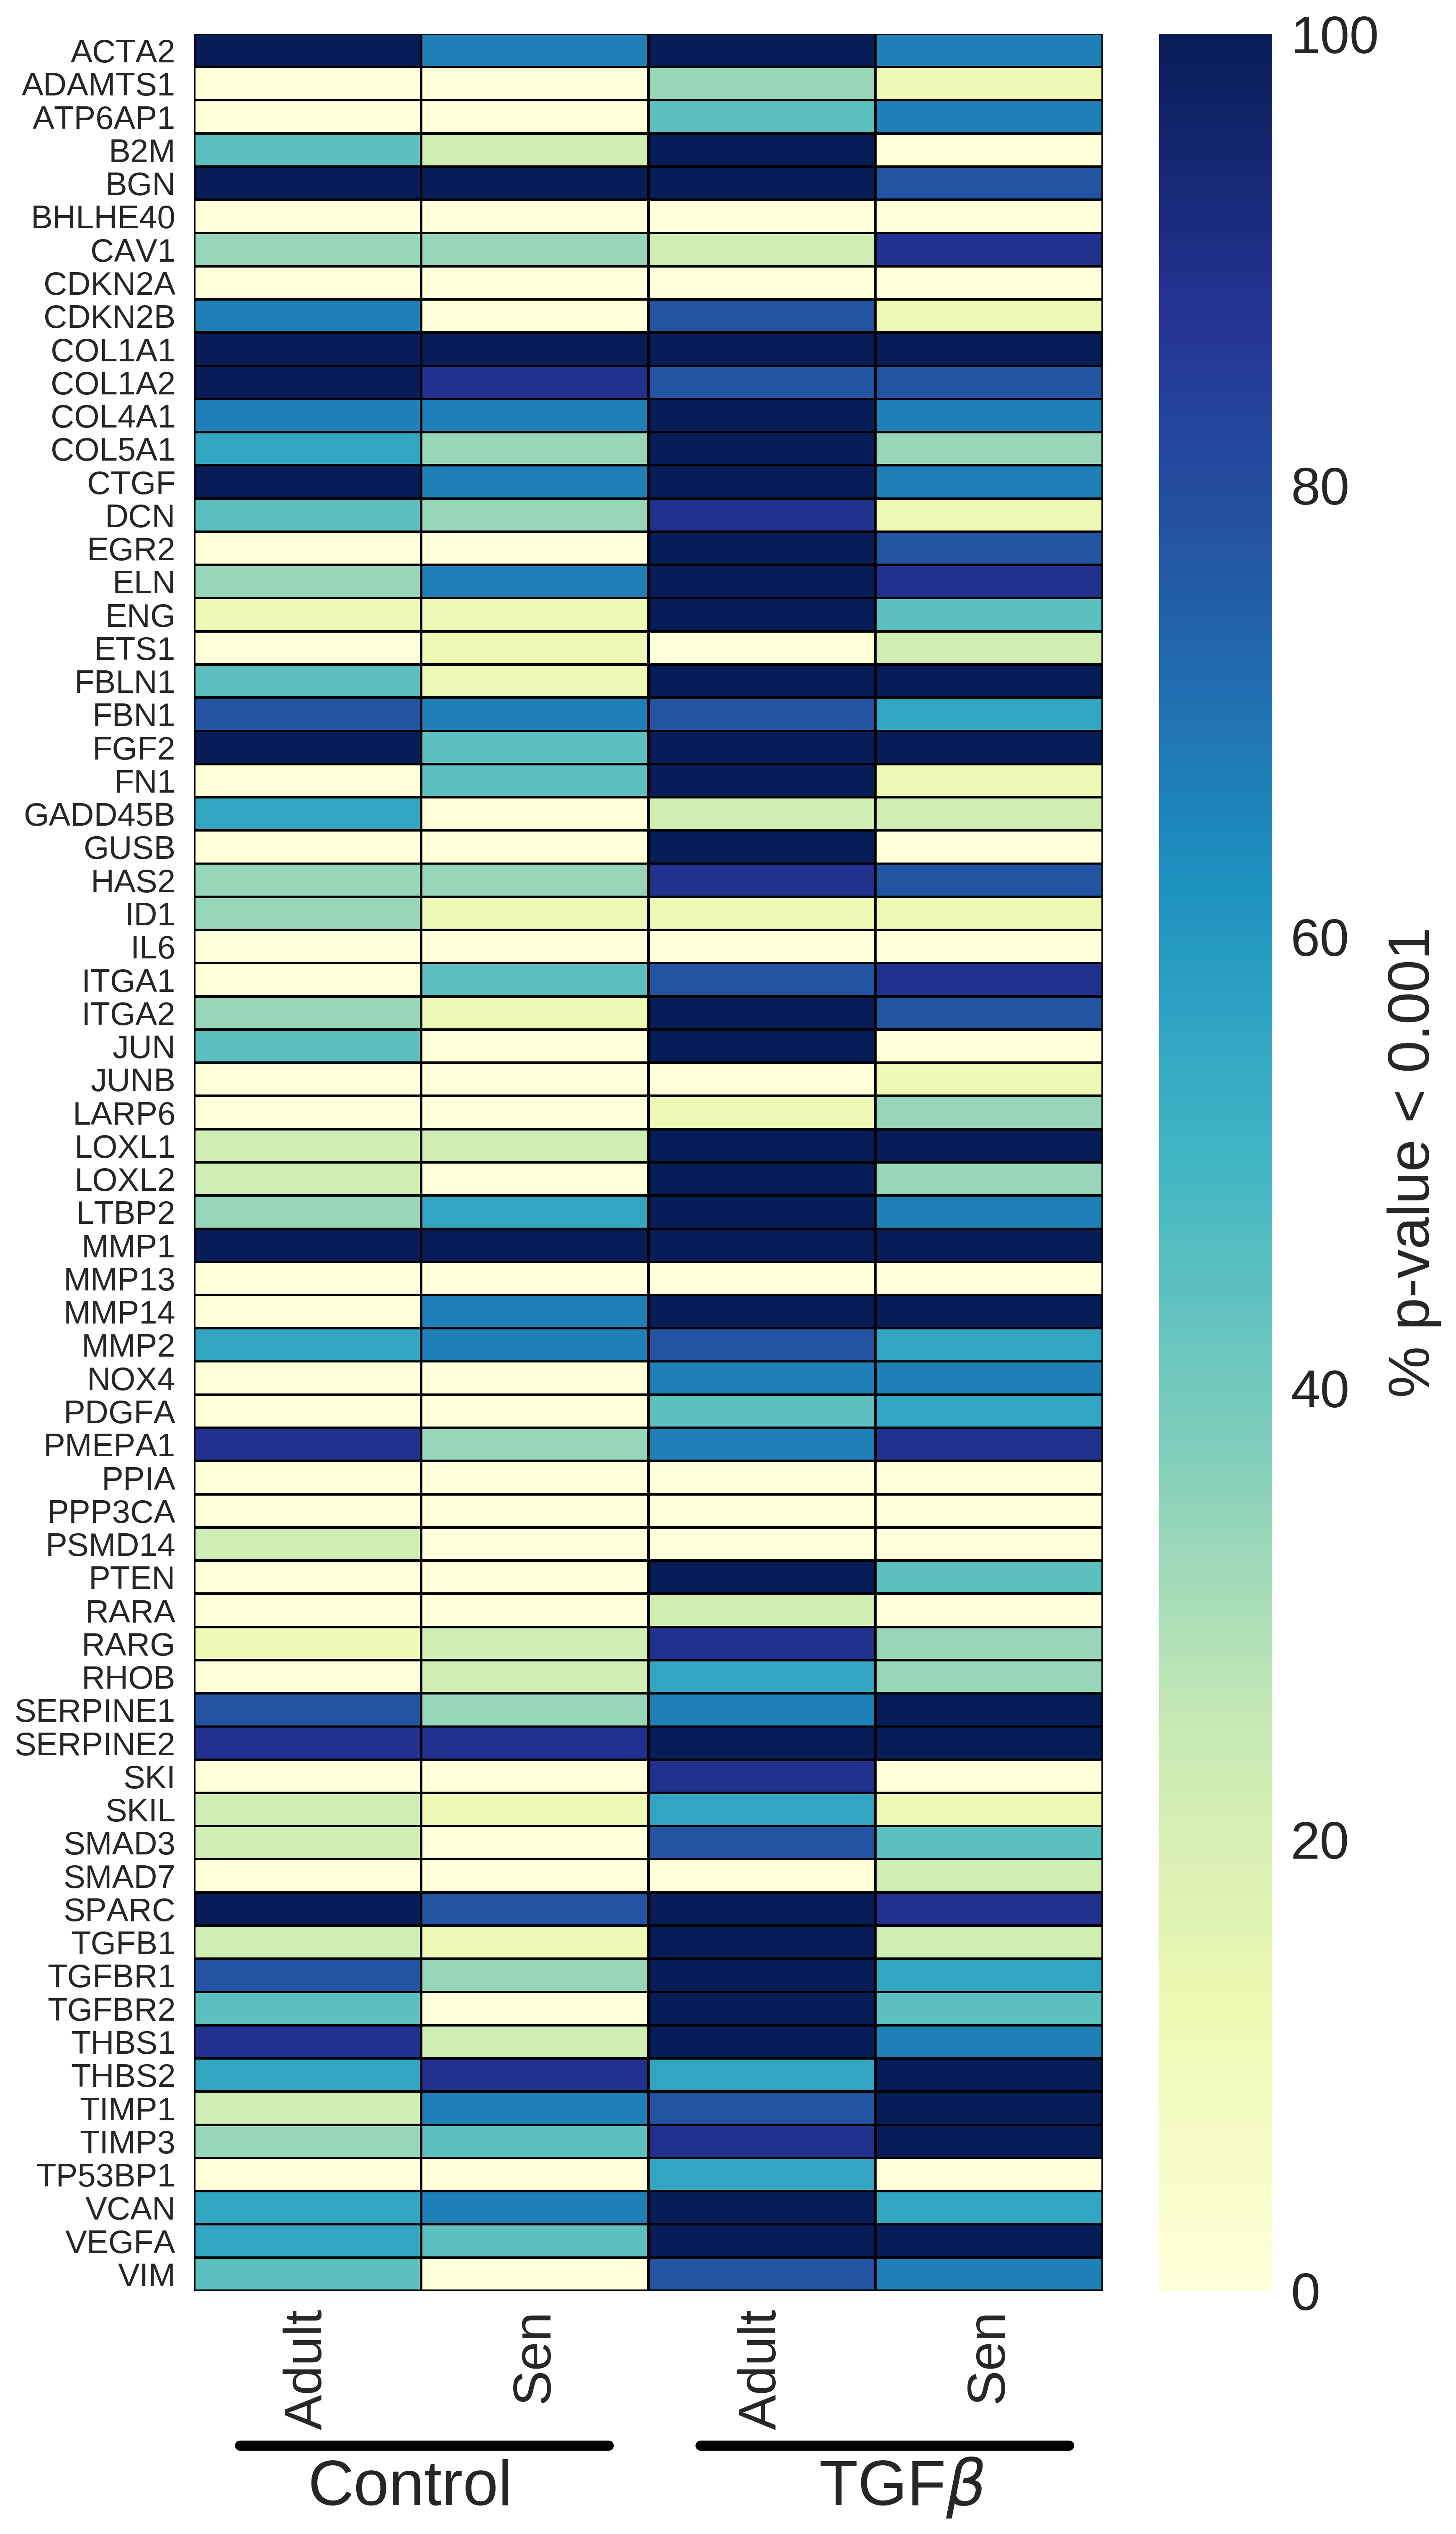
\includegraphics[height=0.7\textheight, width=\linewidth]{LIMMA09_2018/SavedObjects/pval_less_than_0_001/between_heatmap0_001}
		\caption{Between groups comparisons}
		\label{fig:between:heatmap}
	\end{subfigure}
	\begin{subfigure}{0.45\linewidth}
%		\centering
		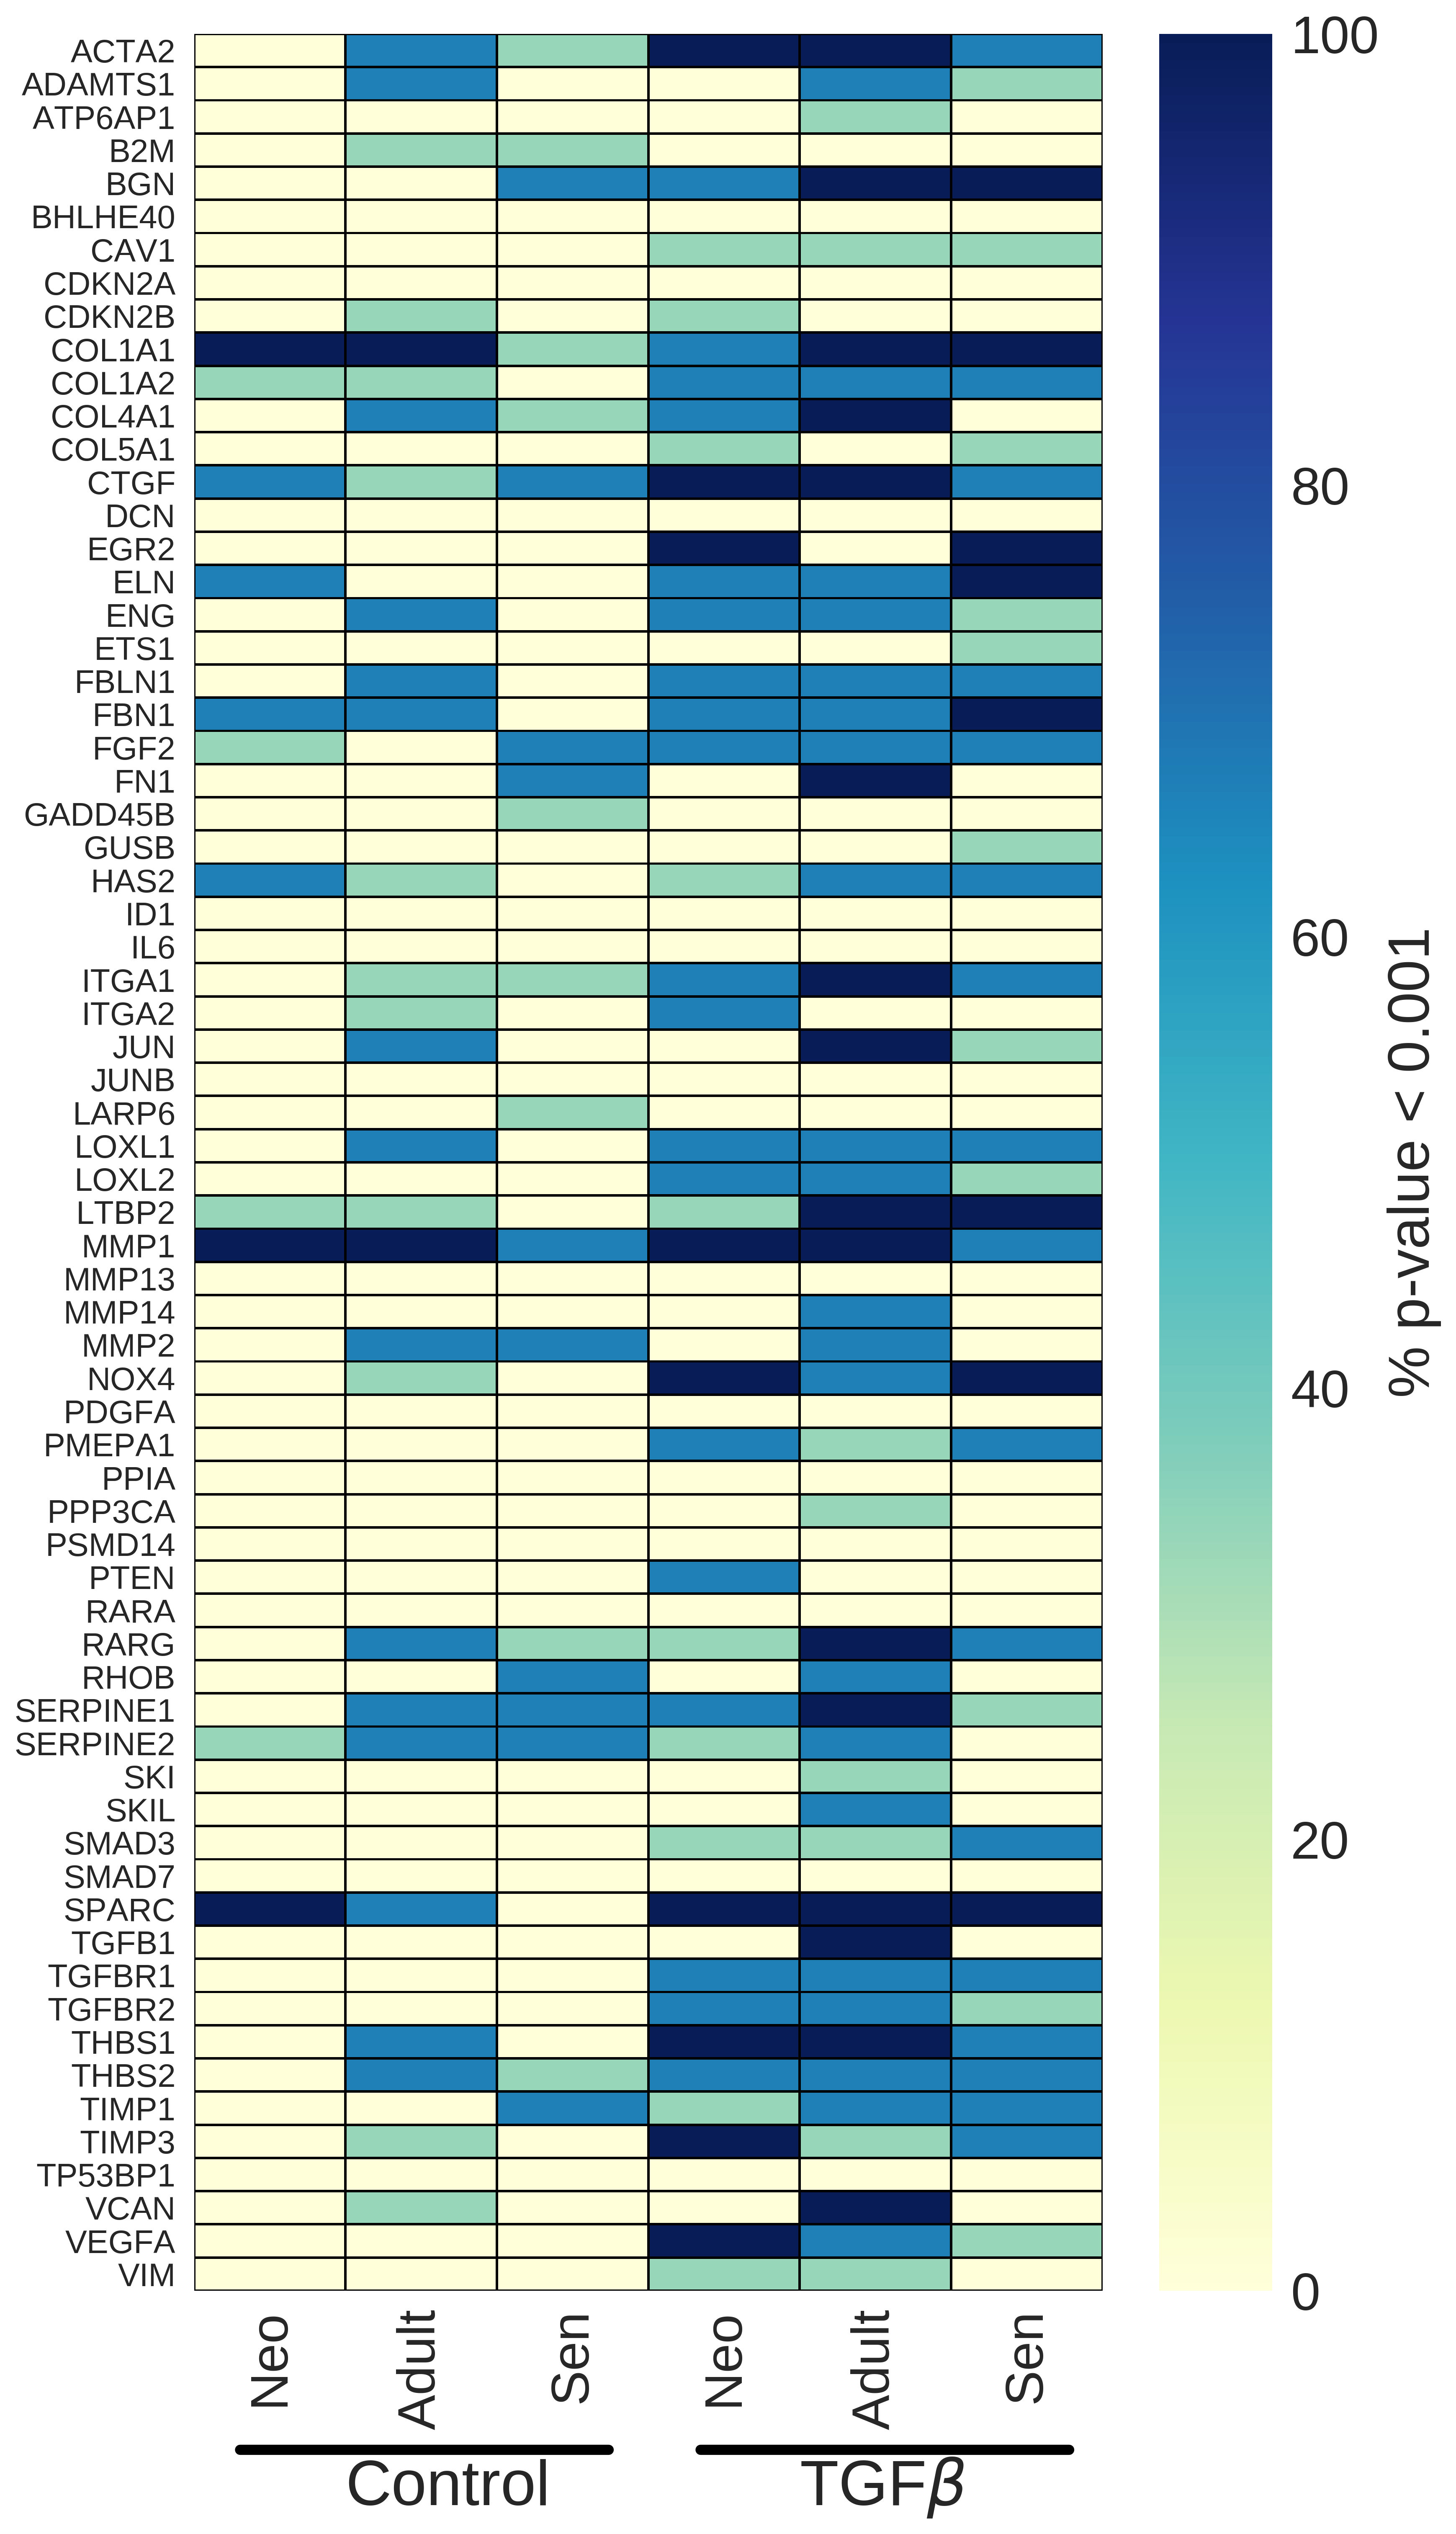
\includegraphics[height=0.7\textheight,width=\linewidth]{LIMMA09_2018/SavedObjects/pval_less_than_0_001/within_heatmap_0_001}
		\caption{Within groups comparisons}
		\label{fig:within:heatmap}
	\end{subfigure}
	\caption{Differential expression analysis for (a) between groups comparisons and (b) within groups comparisons. Colours indicate the percentage of the time of all combinations (9 for between groups and 3 for within groups) of LIMMA analysis conducted that a time series was differentially expressed with a FDR corrected p-value >0.001. }
	\label{fig:heatmap}
\end{figure}

\begin{figure}[p]
	\begin{minipage}{0.9\textwidth}
		\centering
		\begin{subfigure}[b]{0.45\textwidth}
			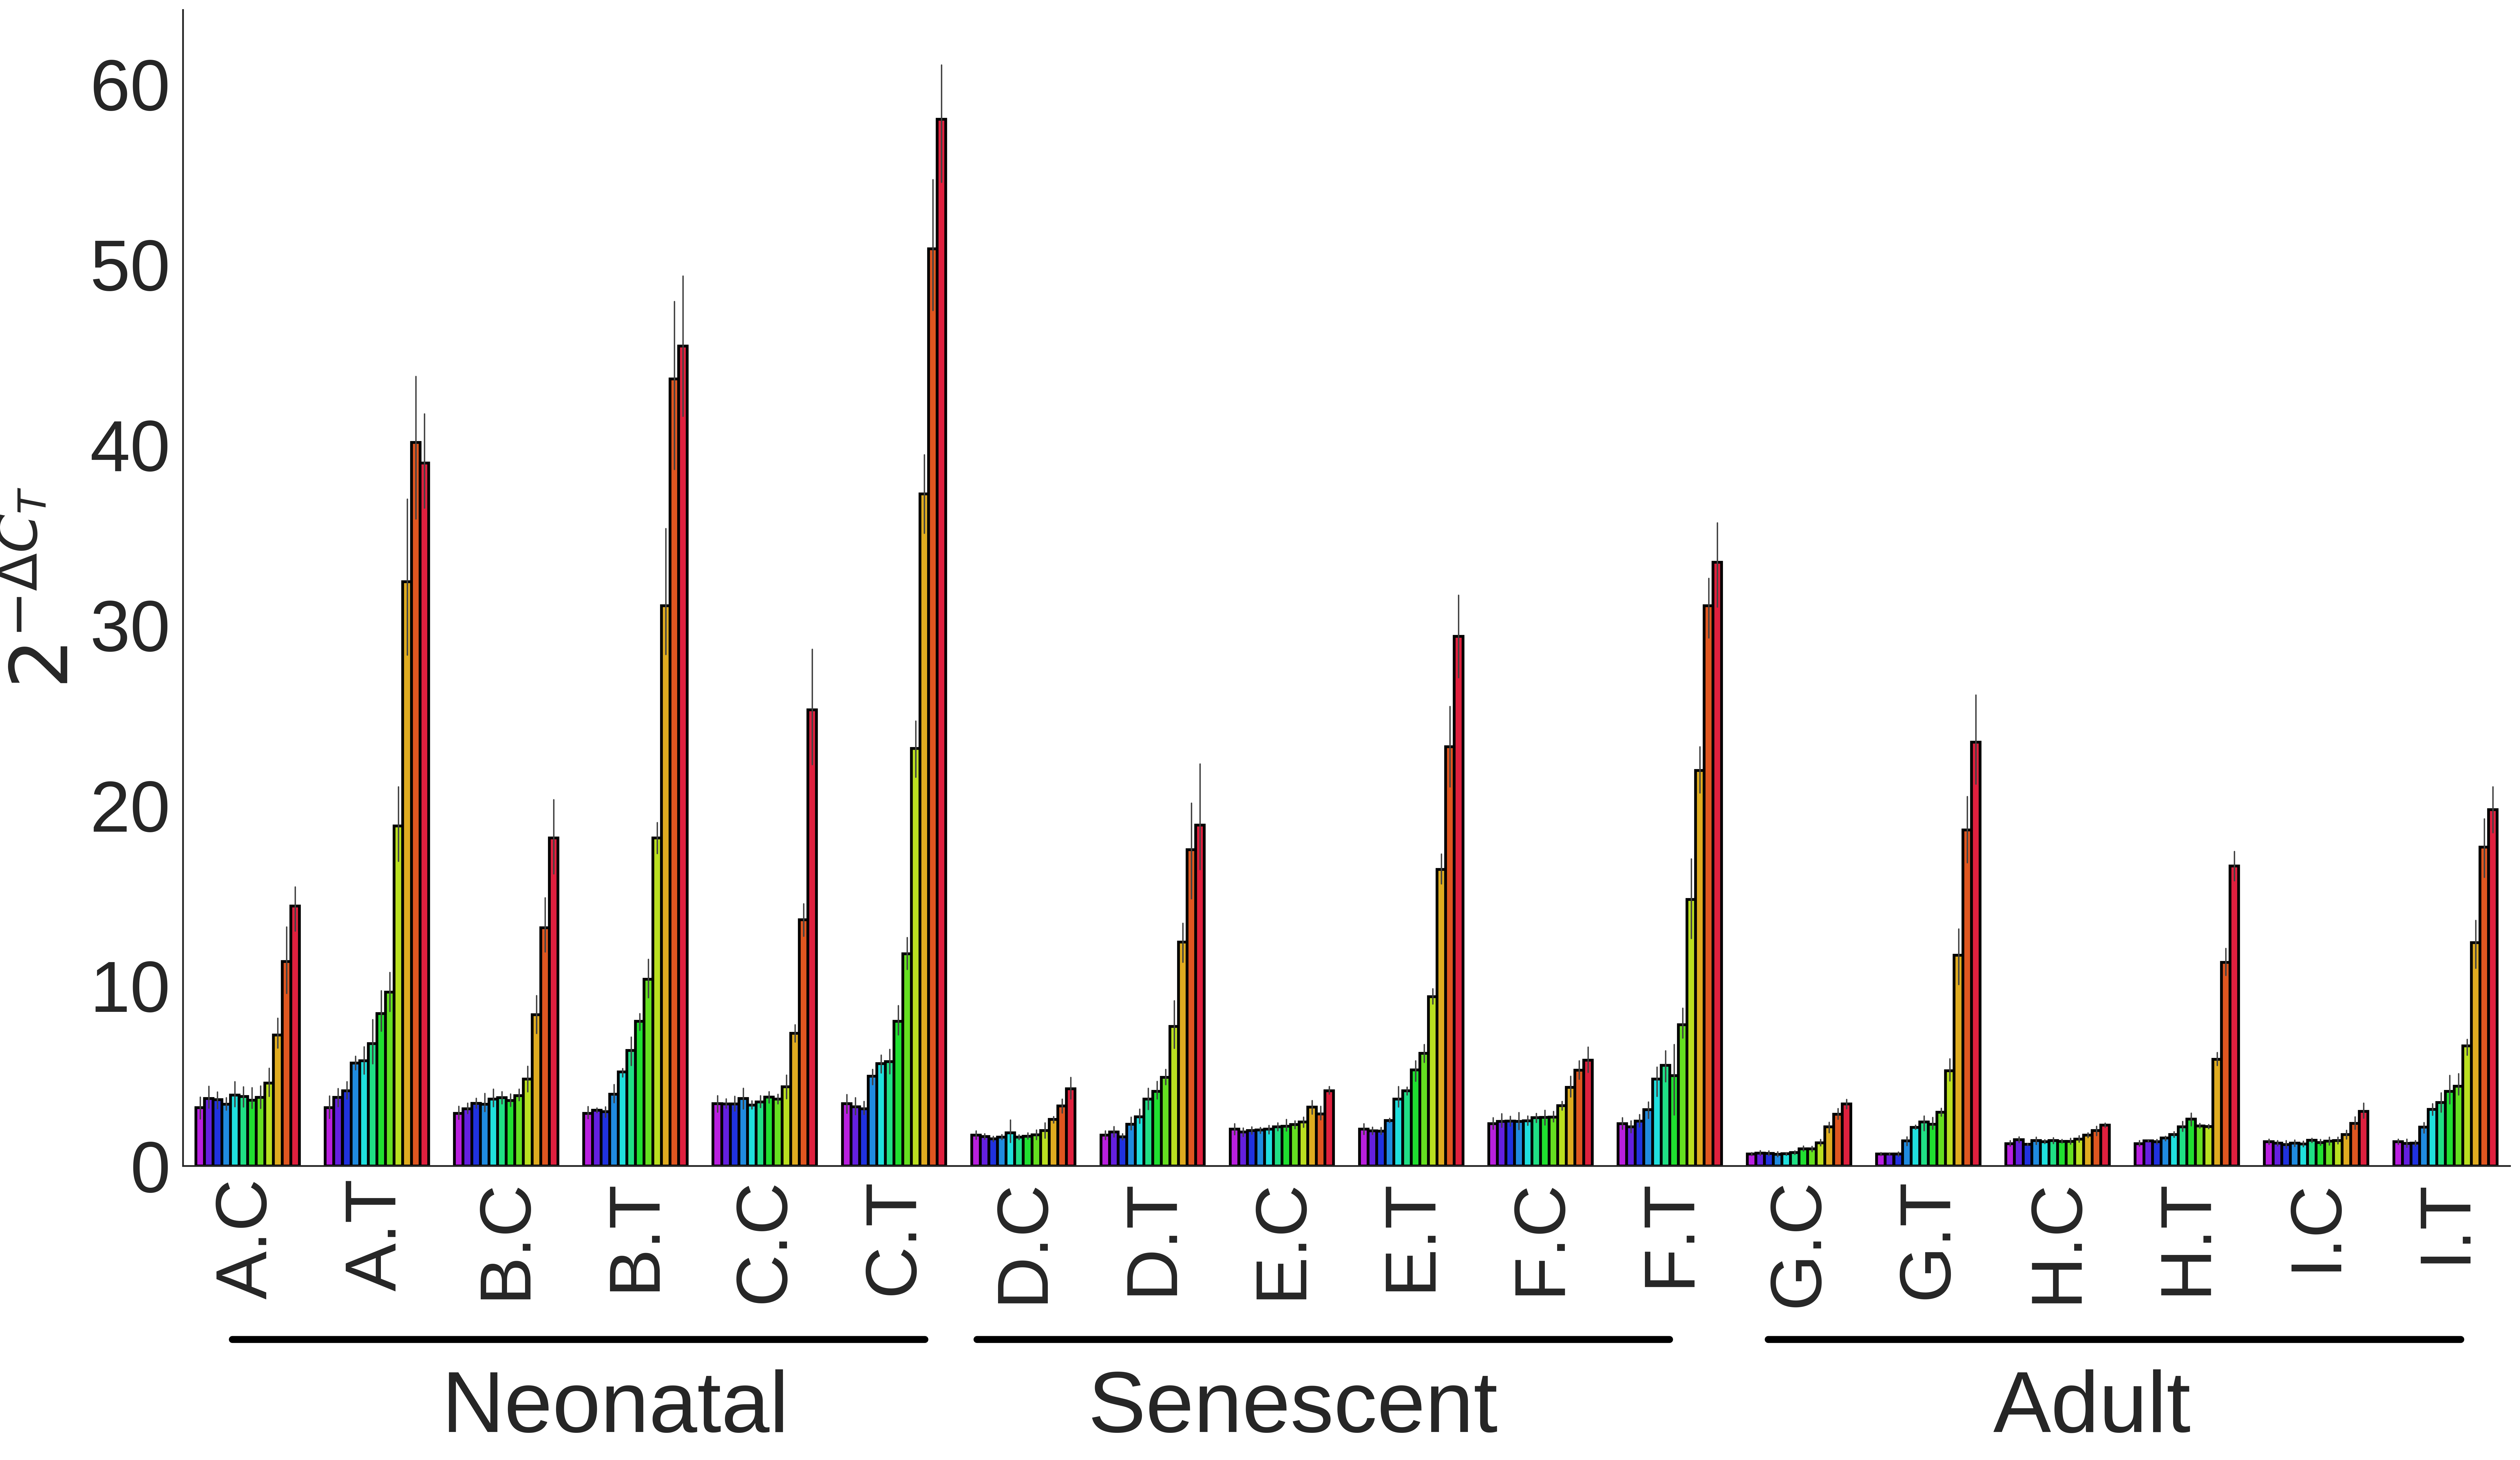
\includegraphics[width=\textwidth]{img/dct_for_publication_no_legend/COL1A1}
			\caption{COL1A1}\label{COL1A1}
		\end{subfigure}\hspace*{\fill}
		\begin{subfigure}[b]{0.45\textwidth}
			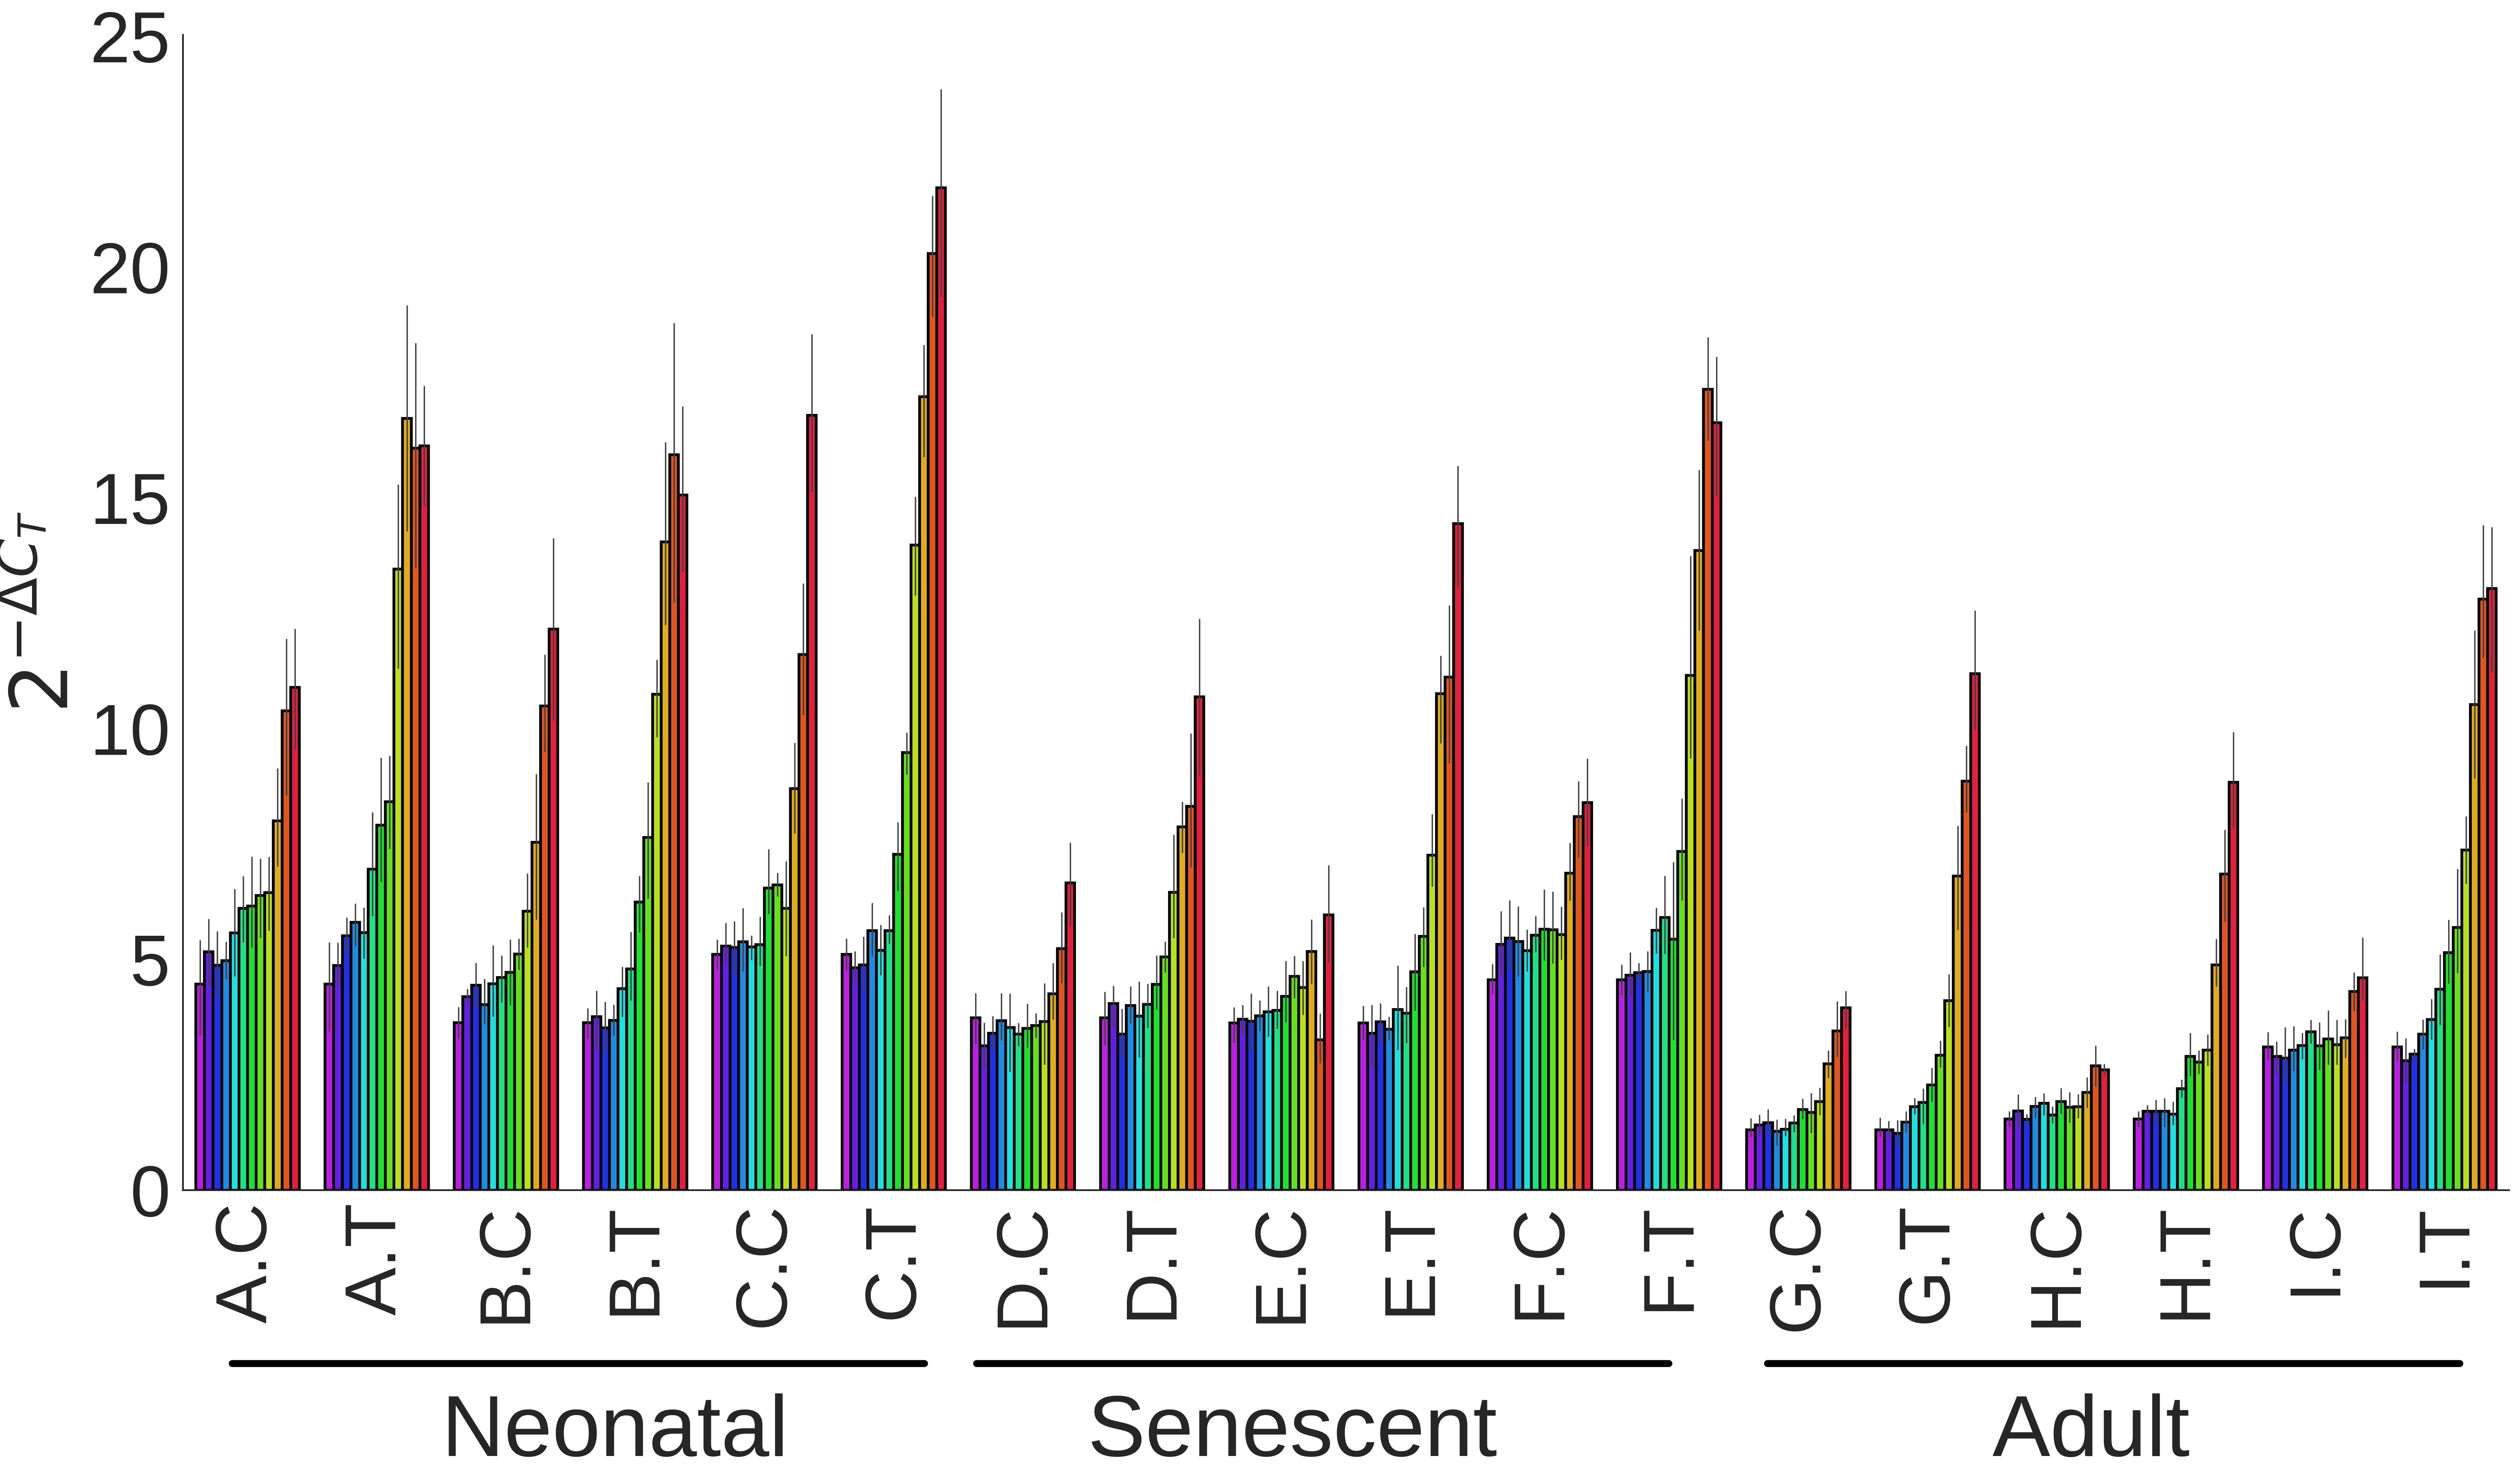
\includegraphics[width=\textwidth]{img/dct_for_publication_no_legend/COL1A2}
			\caption{COL1A2}\label{COL1A2}
		\end{subfigure}\hspace*{\fill}
		
		\begin{subfigure}[b]{0.45\textwidth}
			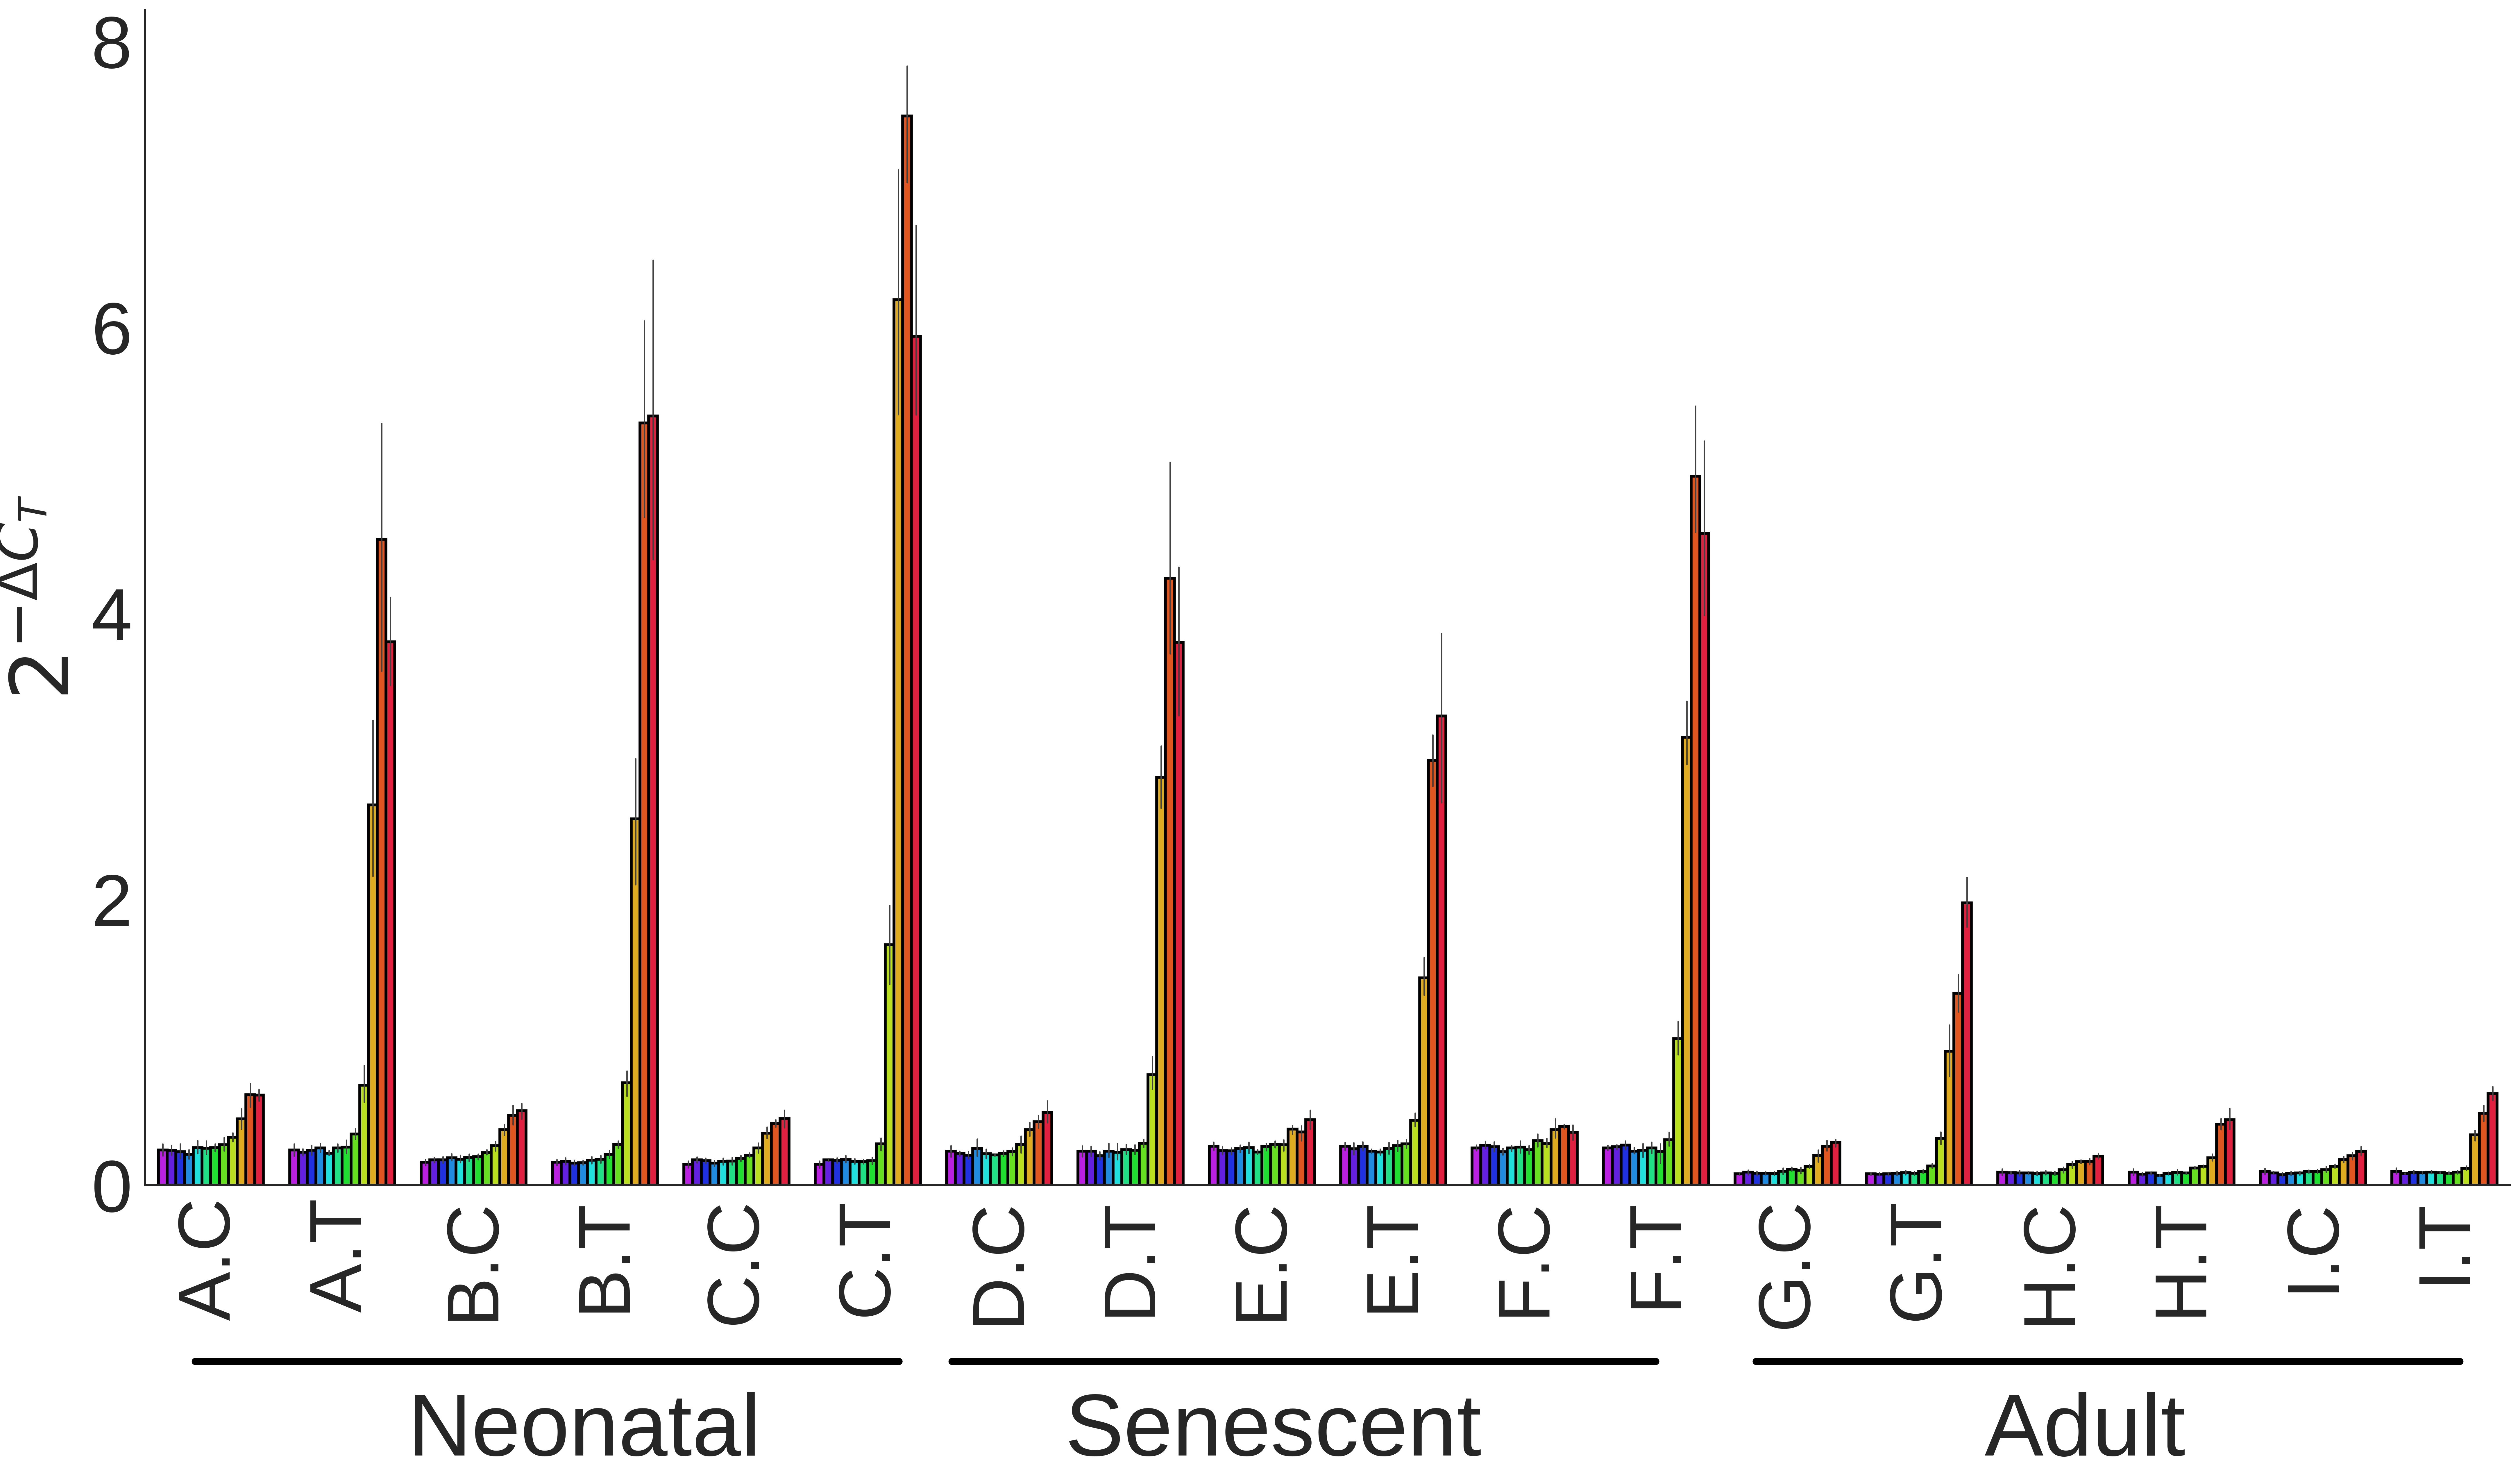
\includegraphics[width=\textwidth]{img/dct_for_publication_no_legend/ACTA2}
			\caption{ACTA2}\label{ACTA2}
		\end{subfigure}\hspace*{\fill}
		\begin{subfigure}[b]{0.45\textwidth}
			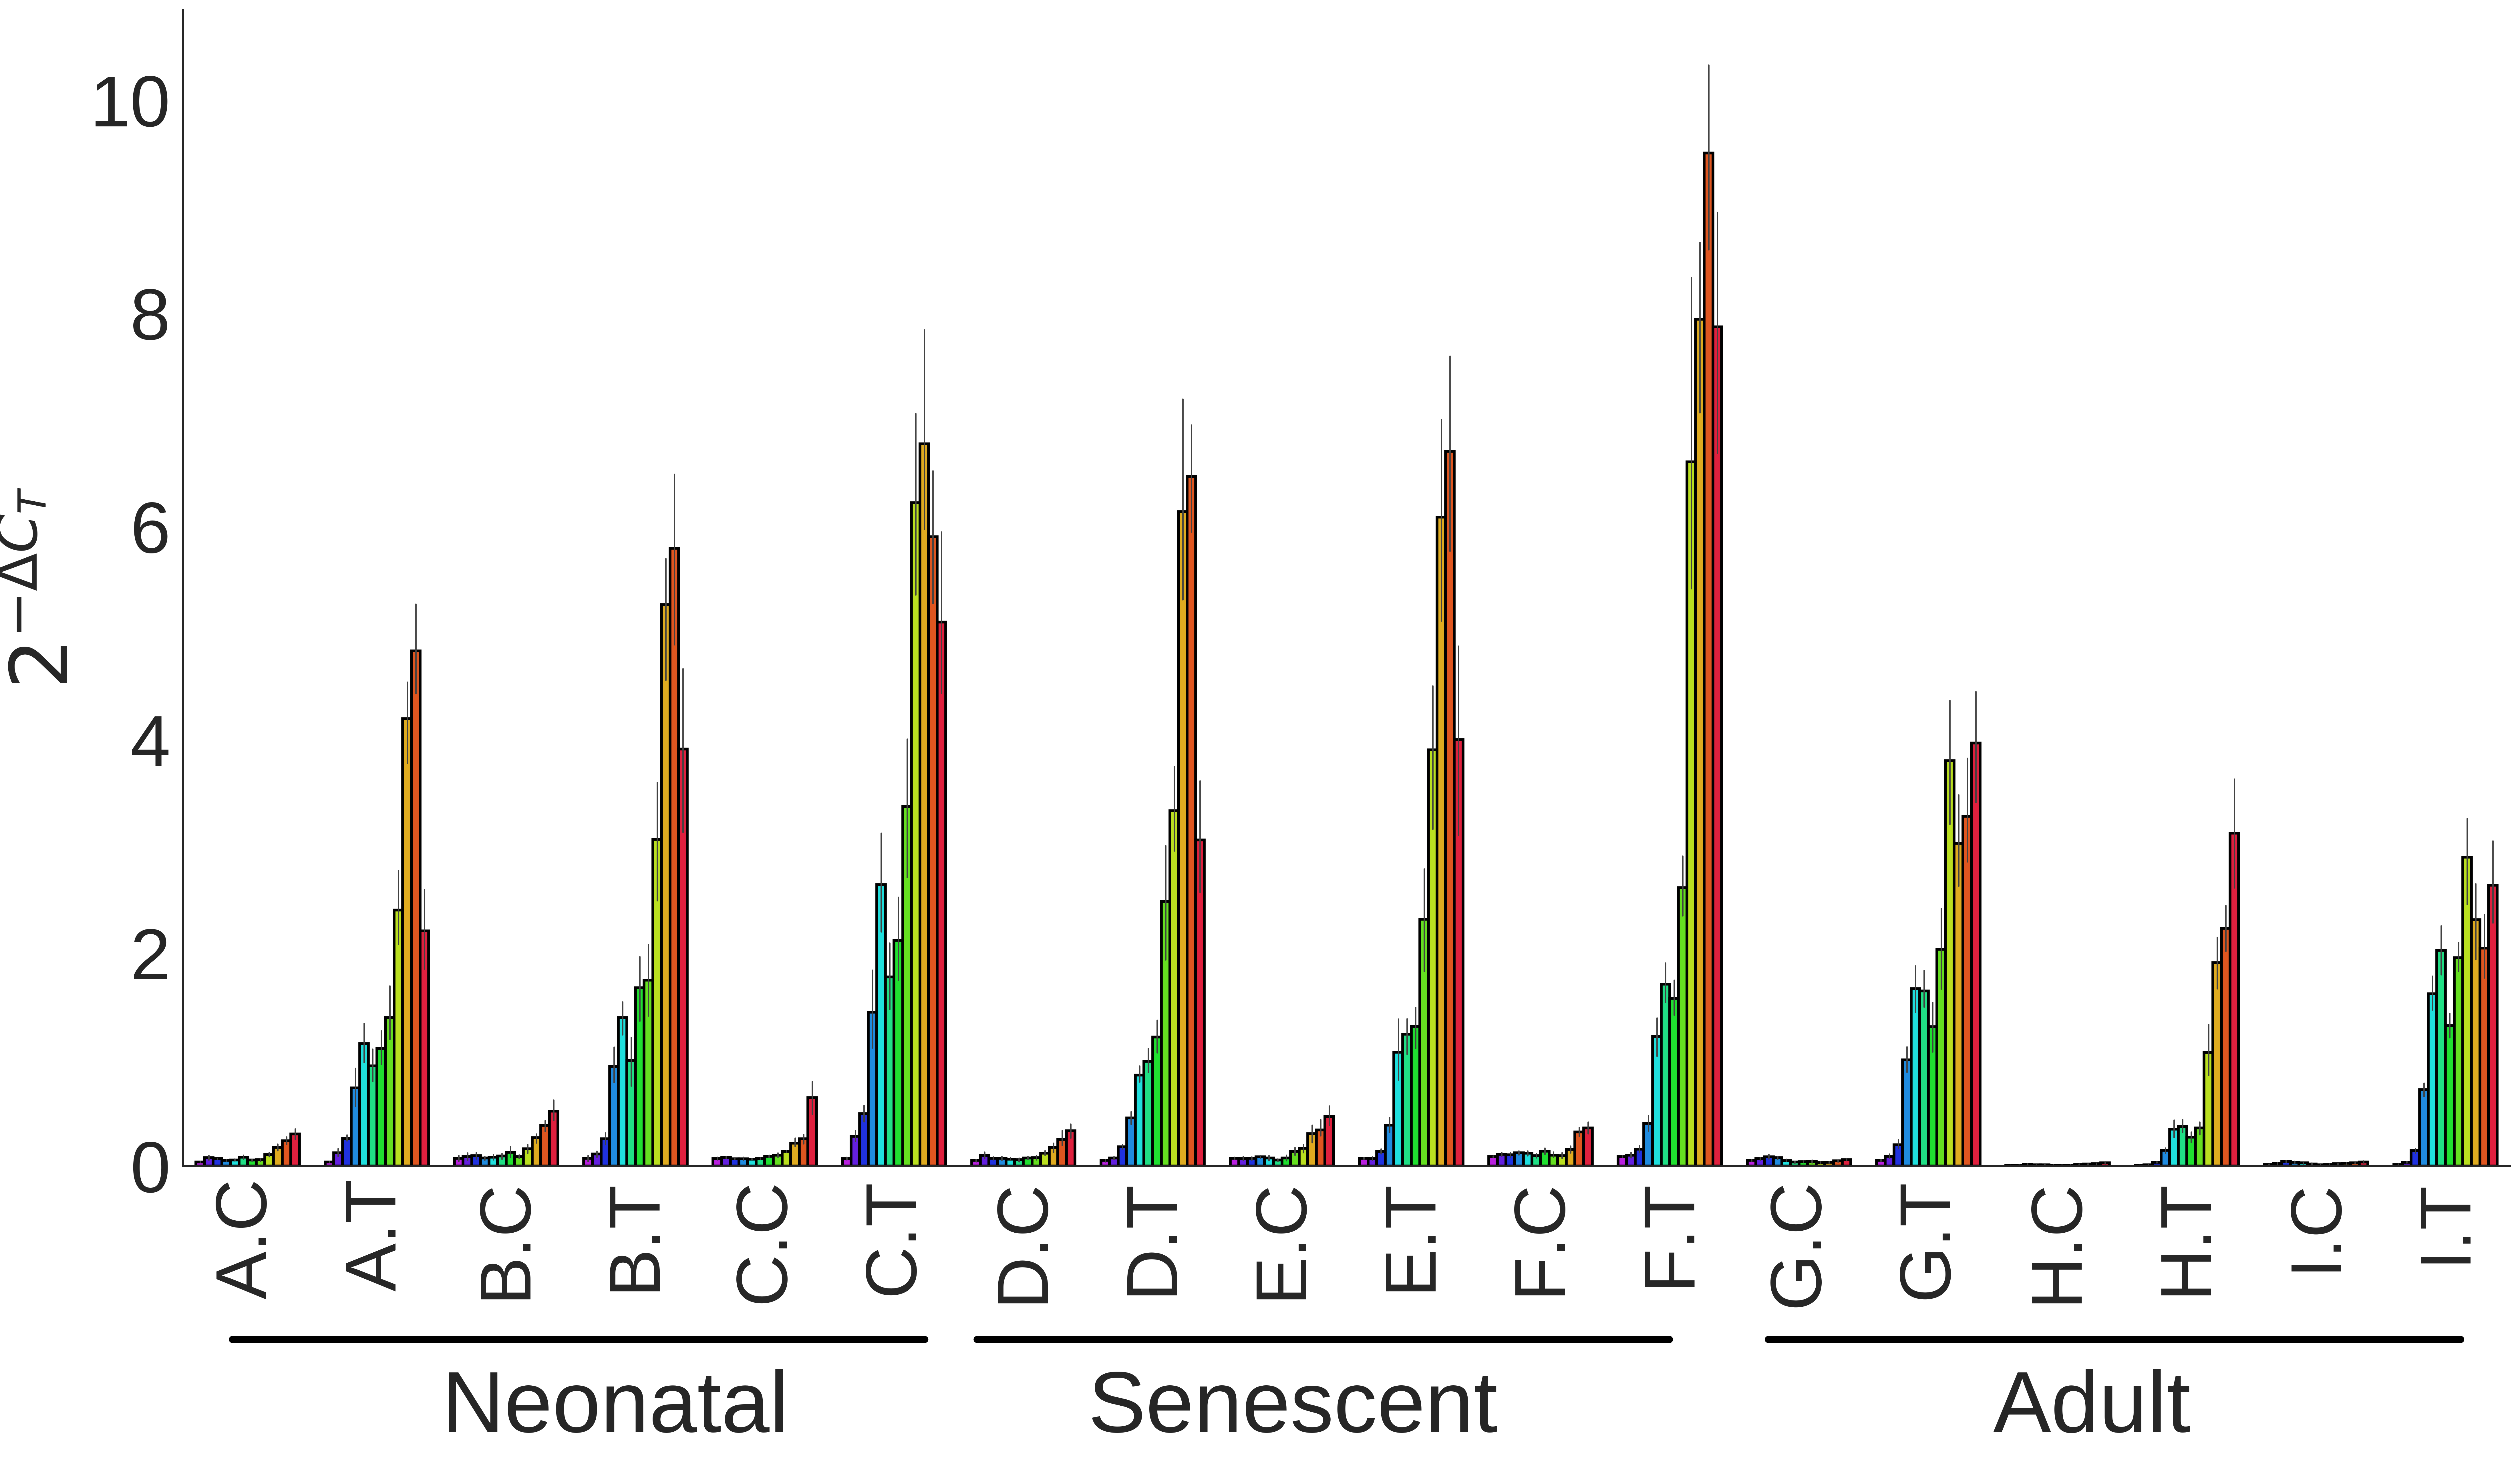
\includegraphics[width=\textwidth]{img/dct_for_publication_no_legend/CTGF}
			\caption{CTGF}\label{CTGF}
		\end{subfigure}\hspace*{\fill}
		
		\begin{subfigure}[b]{0.45\textwidth}
			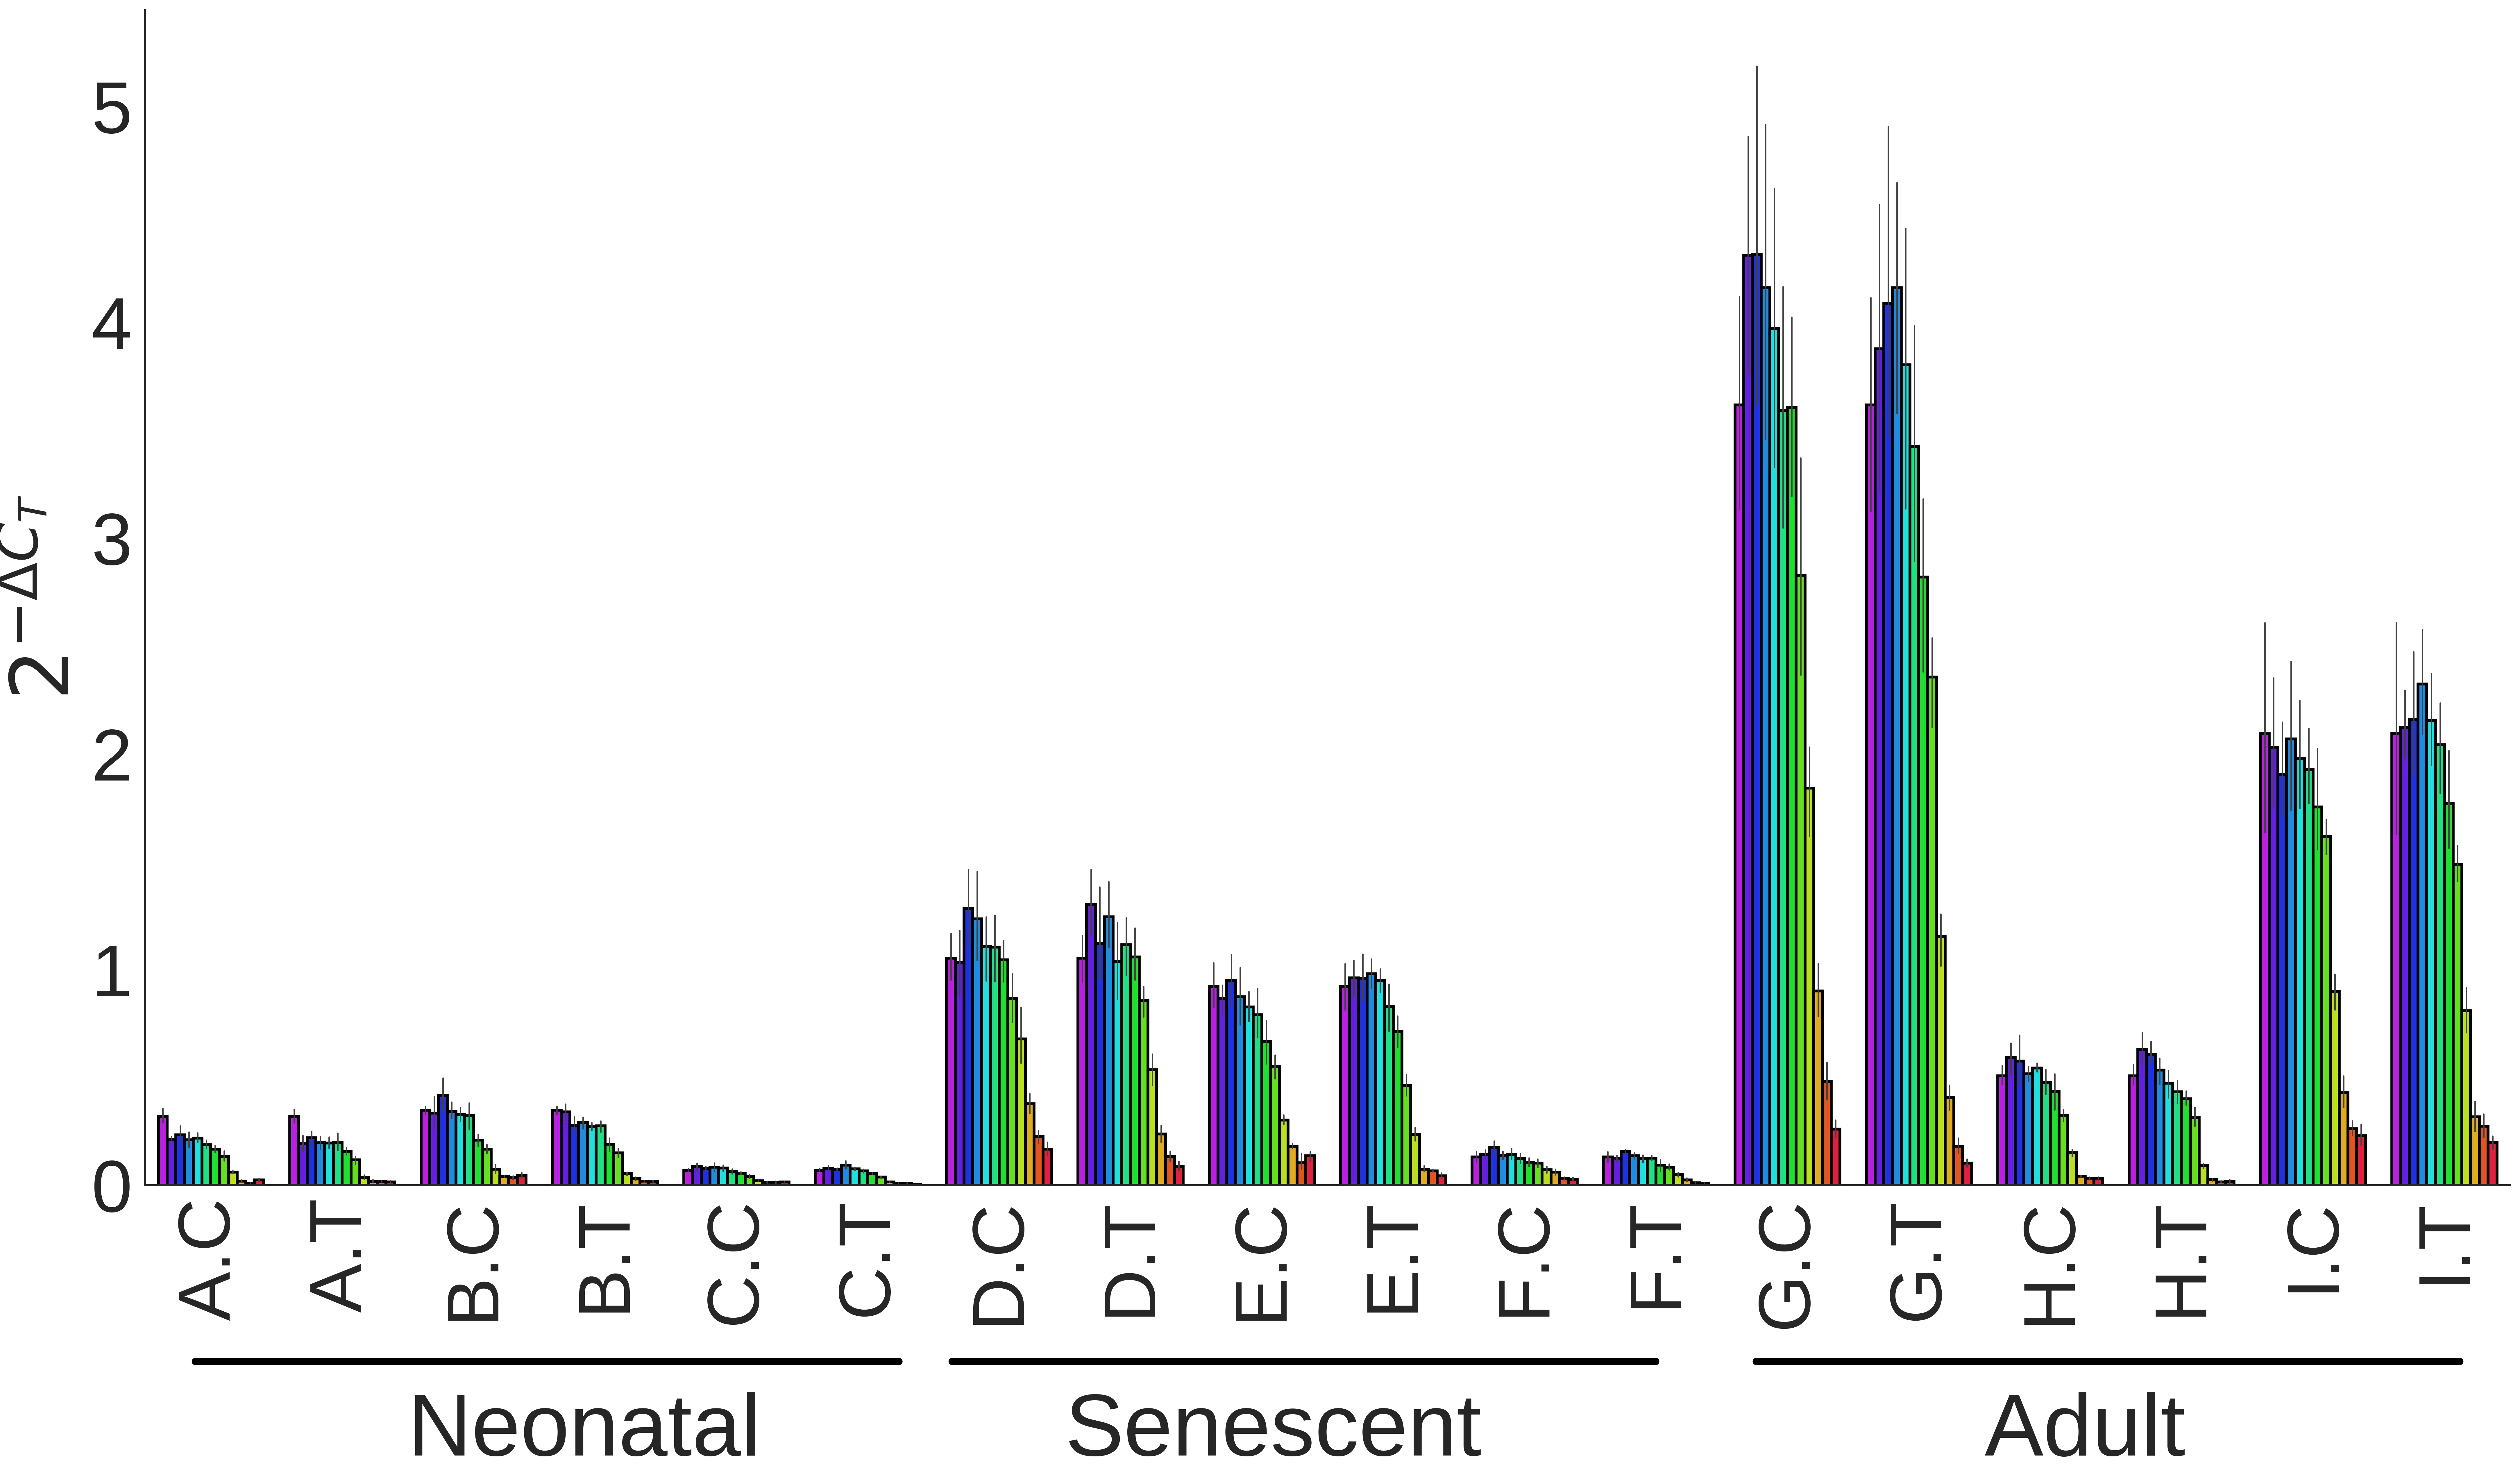
\includegraphics[width=\textwidth]{img/dct_for_publication_no_legend/MMP1}
			\caption{MMP1}\label{MMP1}
		\end{subfigure}\hspace*{\fill}
		\begin{subfigure}[b]{0.45\textwidth}
			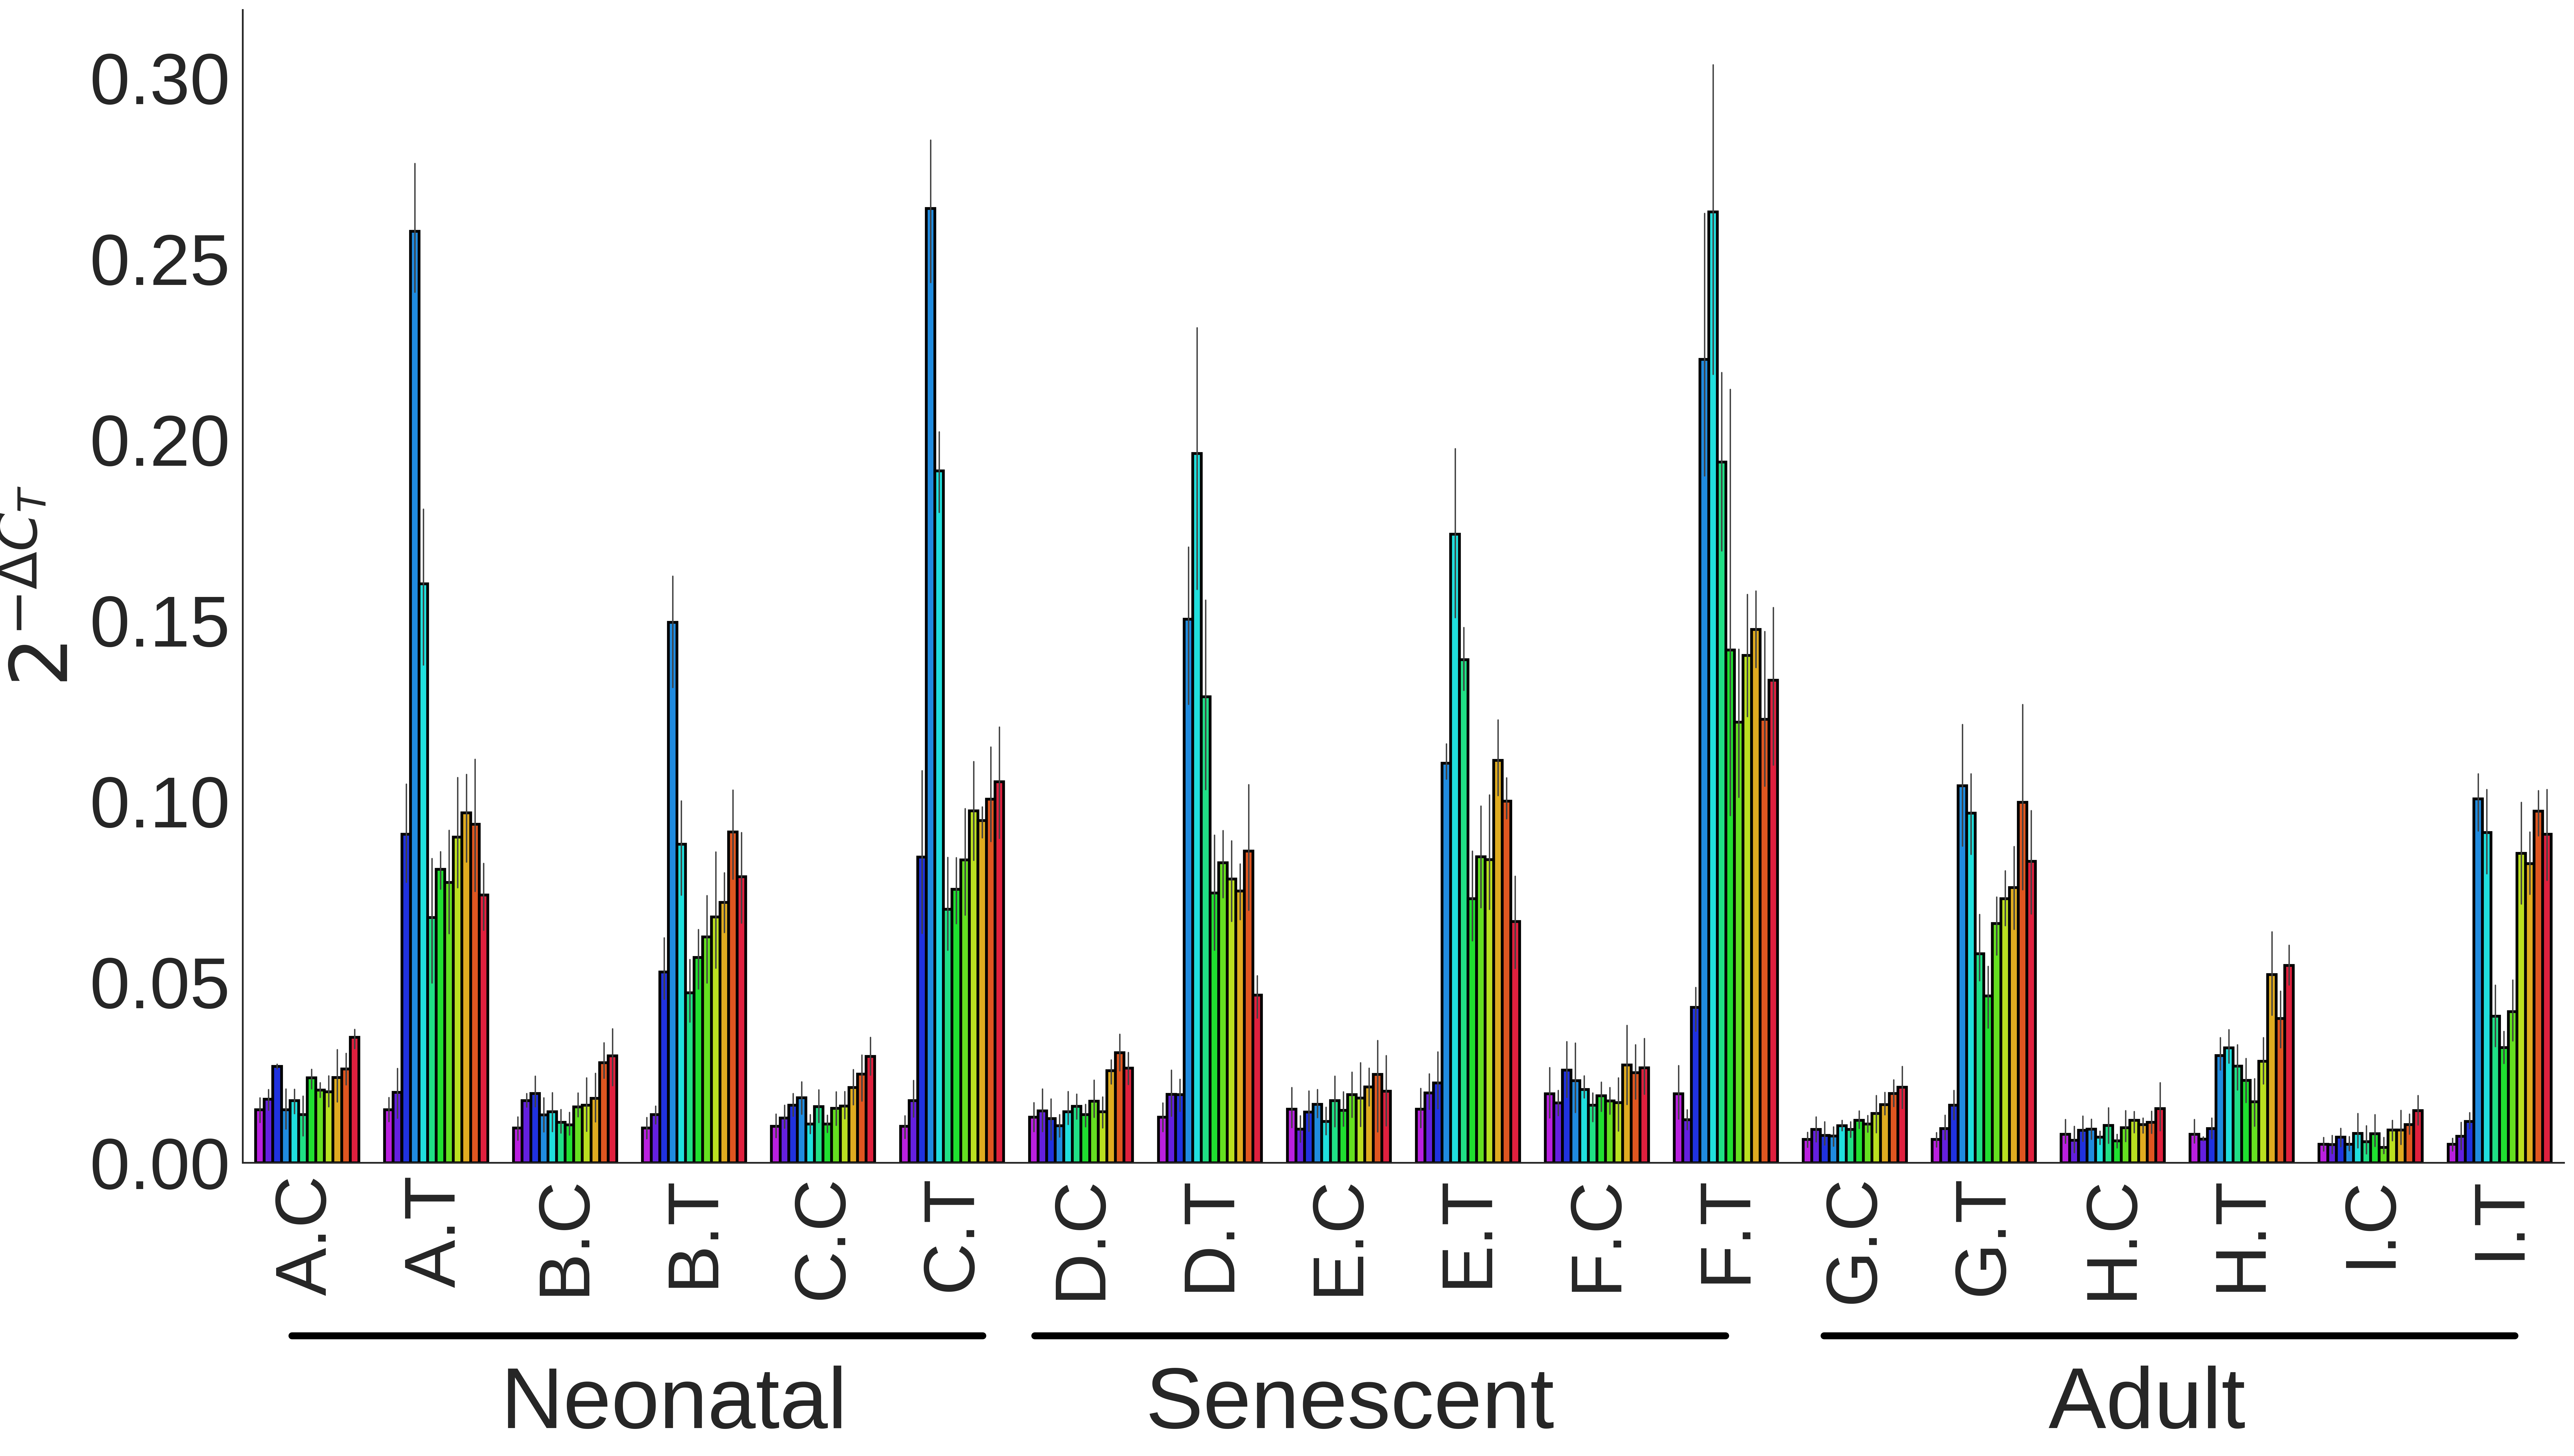
\includegraphics[width=\textwidth]{img/dct_for_publication_no_legend/SMAD7}
			\caption{SMAD7}\label{SMAD7}
		\end{subfigure}\hspace*{\fill}
		
		\begin{subfigure}[b]{0.45\textwidth}
			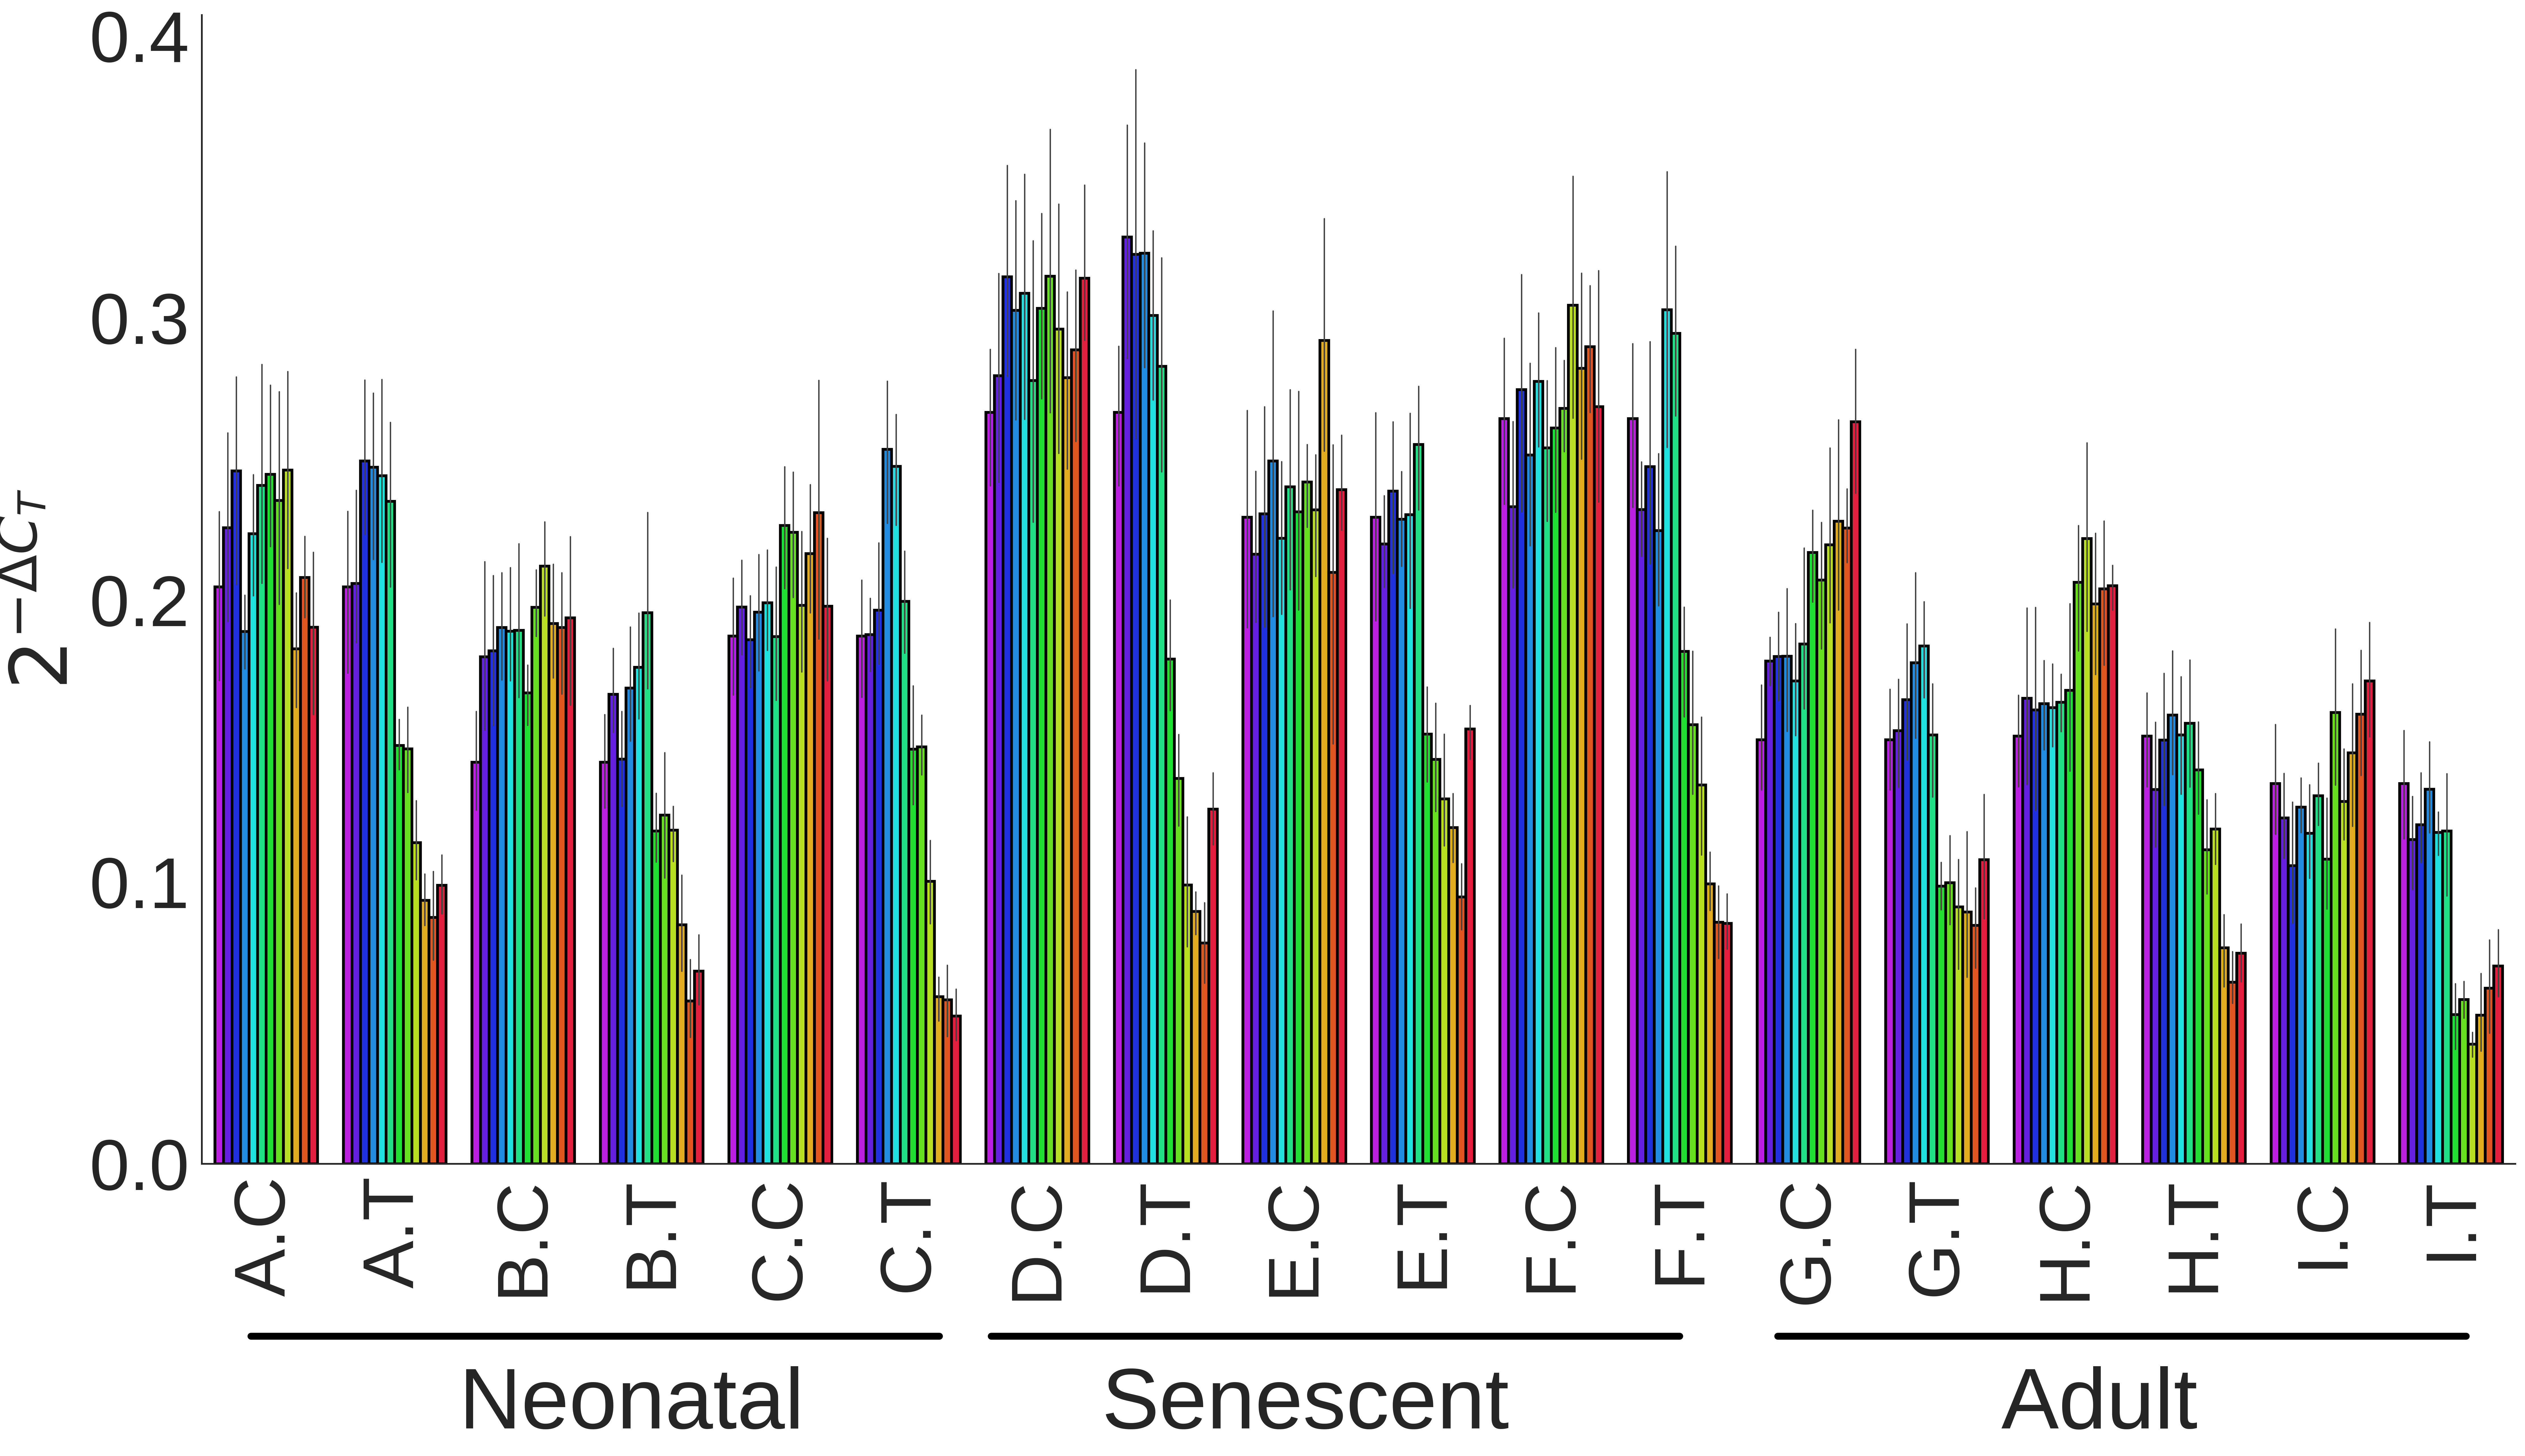
\includegraphics[width=\textwidth]{img/dct_for_publication_no_legend/SMAD3}
			\caption{SMAD3}\label{SMAD3}
		\end{subfigure}\hspace*{\fill}
		\begin{subfigure}[b]{0.45\textwidth}
			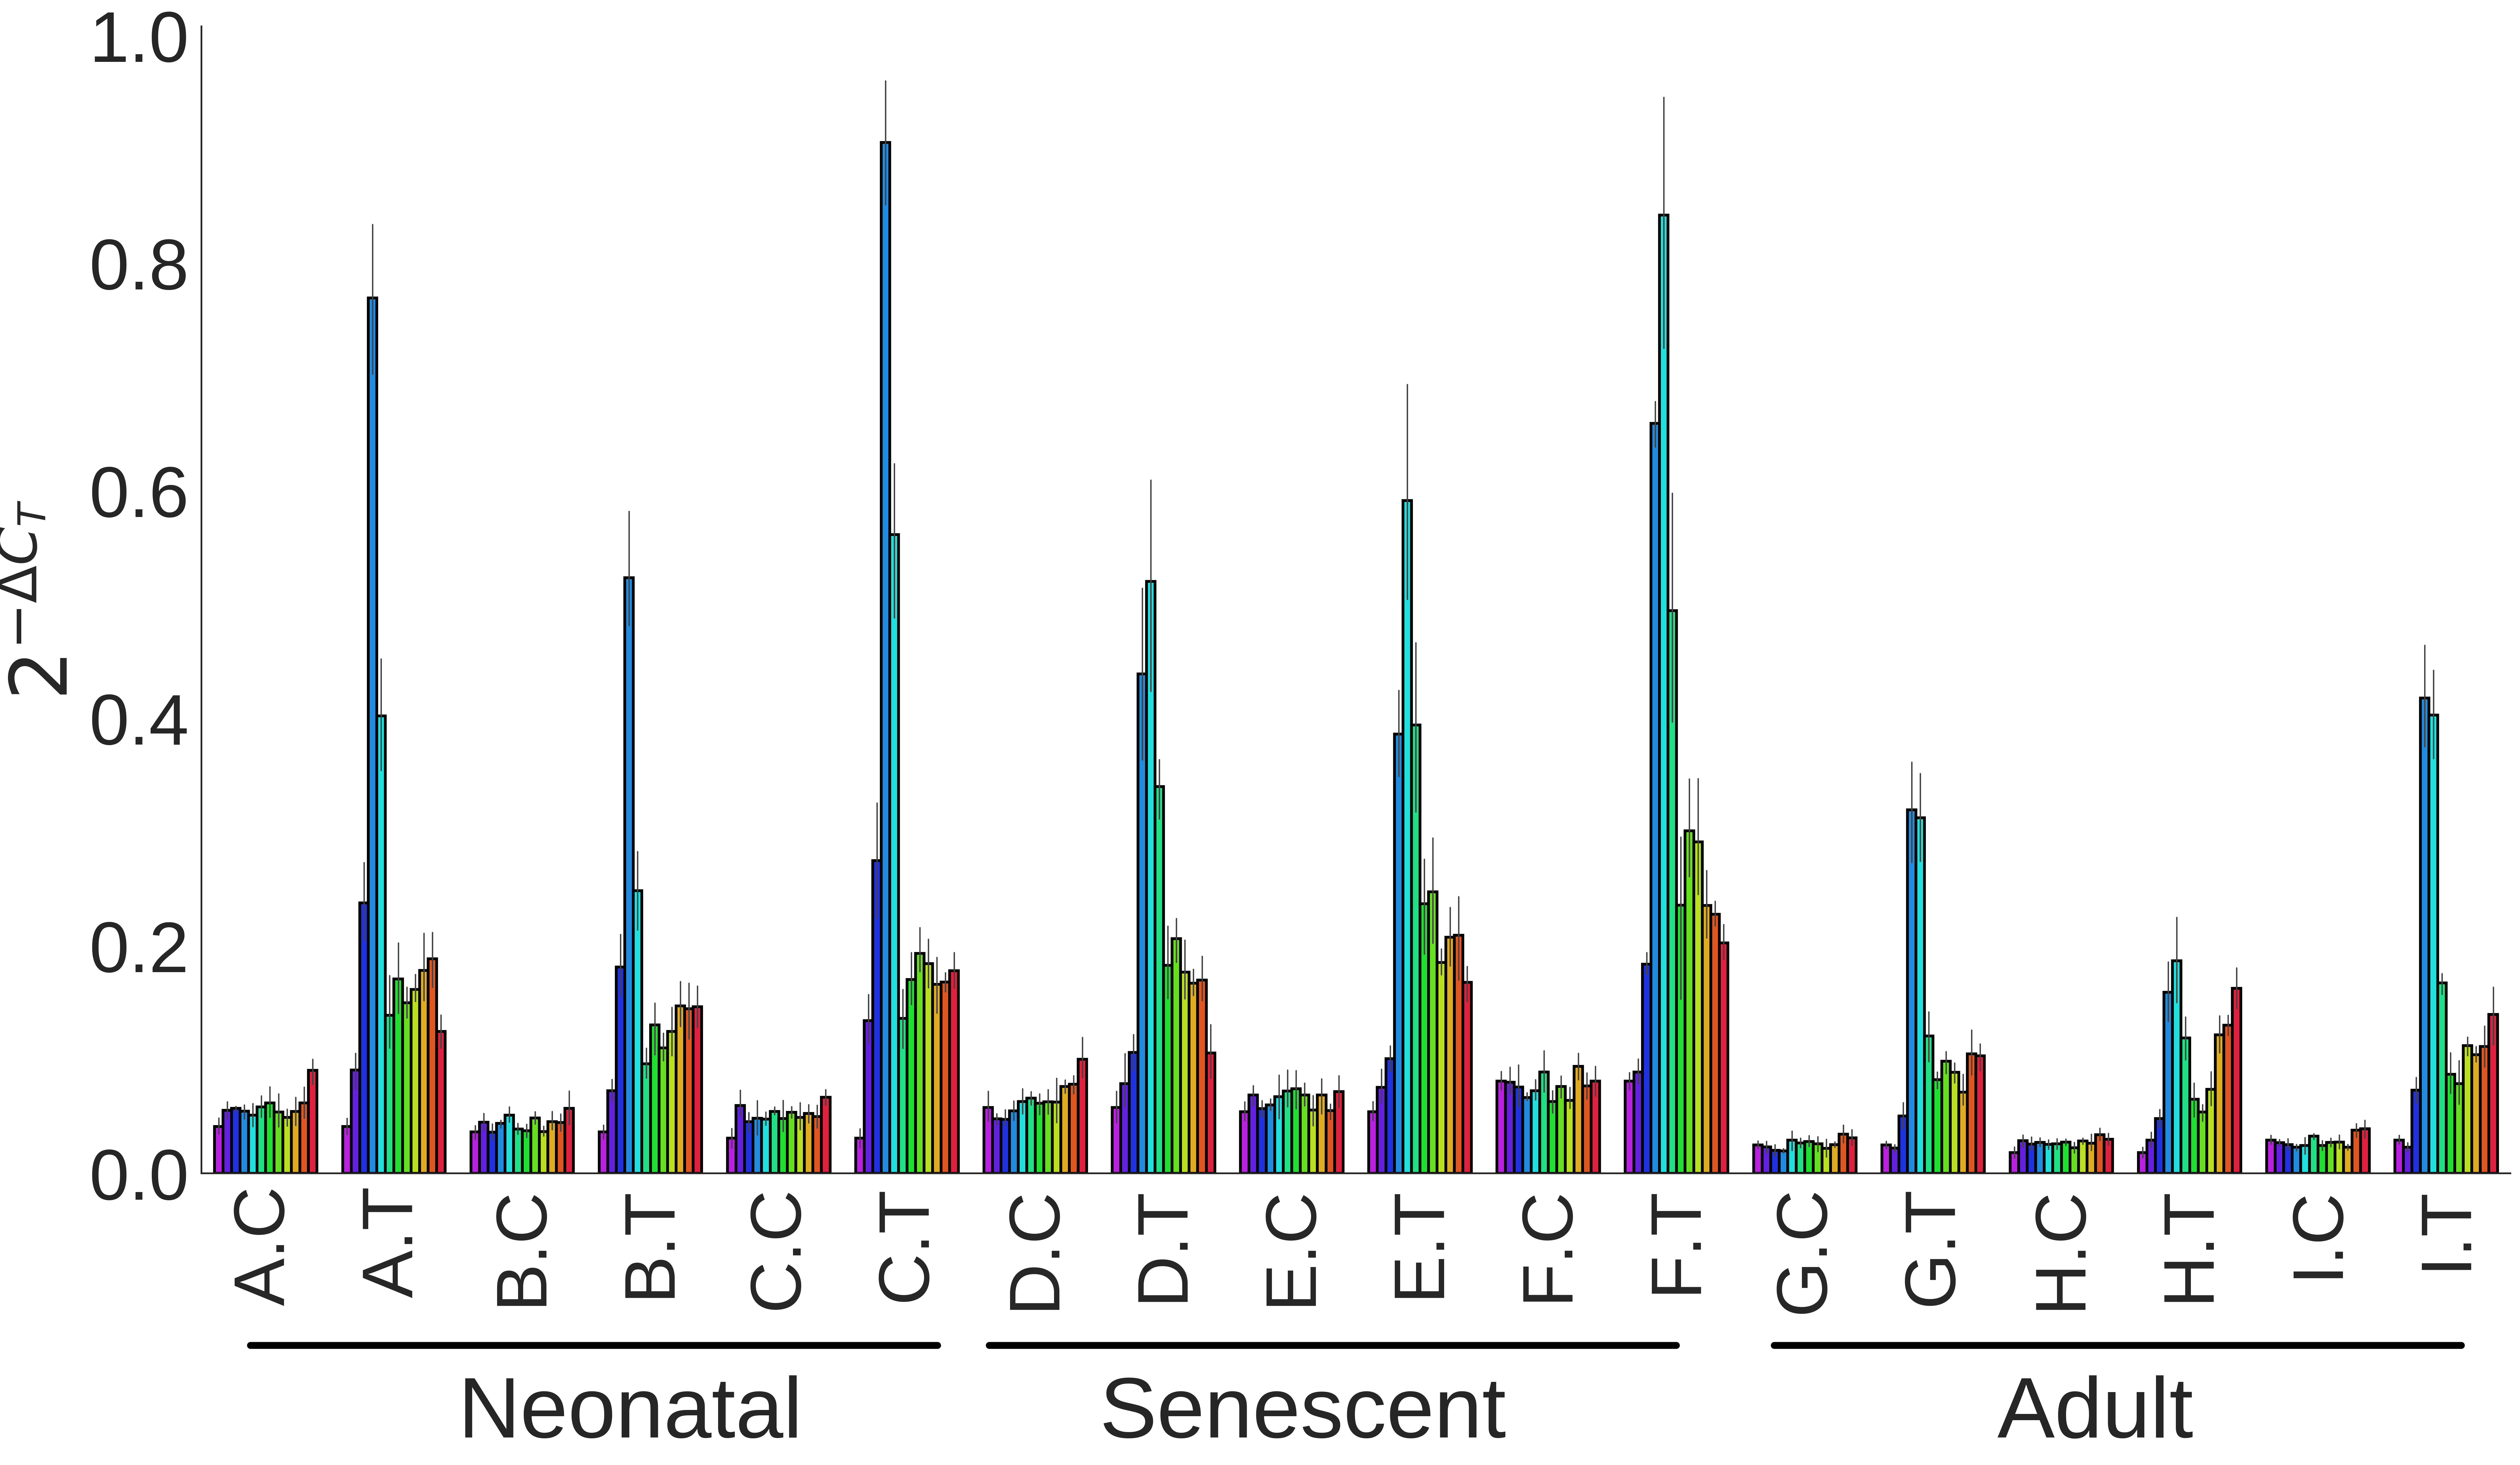
\includegraphics[width=\textwidth]{img/dct_for_publication_no_legend/JUNB}
			\caption{JUNB}\label{JUNB}
		\end{subfigure}\hspace*{\fill}
	\end{minipage}% <--- don't forget
	\begin{minipage}{0.1\textwidth}
		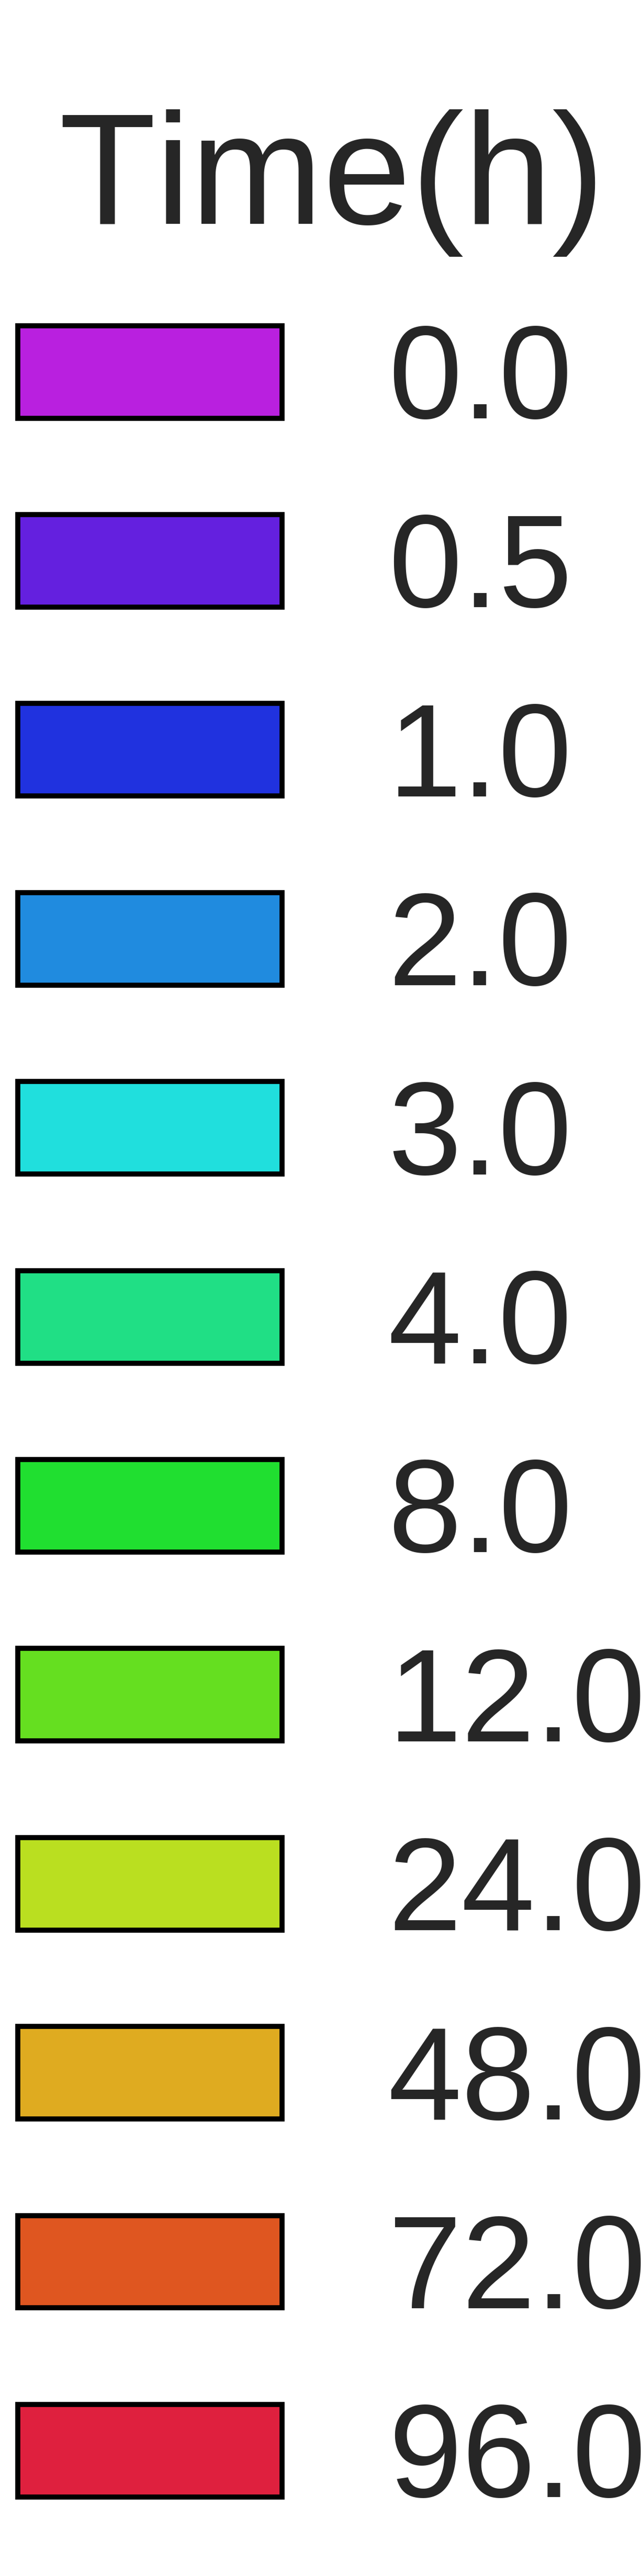
\includegraphics[width=\textwidth,height=8cm]{img/dct_for_publication_no_legend/legend}
	\end{minipage}
	\caption{Bar graphs showing control (C) and \tgf{} (T) treated time series datasets for each cell line (labelled A-I as described in the methods). Error bars represent standard error of the mean and each conditions was repeated 6 times.}
	\label{fig:bar_graphs}
\end{figure}

%\subsubsection{A selection of gene measurements with detailed temperol dynamics}
\cref{fig:bar_graphs} shows a selection of the genes measured in this experiment. For a pdf document containing similar but full sized graphs for each measured gene, please see supplementary file 1. 

Collagen 1A1 and 1A2 were produced as a consequence of time in culture \cref{COL1A1, COL1A2} and were strongly induced by \tgf{}. Neonatal cell lines produced more collagens than both adult and senescent cell lines. 

ACTA2 $\upalpha$-SMA and CTGF were both among the most strongly induced of the genes measured. \tgf{} strongly induced both ACTA2 \cref{ACTA2} and CTGF \cref{CTGF} in all cell lines but the induction was considerably weaker in adult cell lines (\cref{ACTA2}). 

Senescent cell lines produced more MMP1 than neonatal cell lines while adult cells variably produced more MMP1 than both neonatal and senescent cell lines \cref{MMP1}. The time series profile in all cell lines were similar in shape, but not in magnitude and \tgf{} did not modulate the transcription of MMP1. 

Smad7 is present in very small quantities without the presence of \tgf{} while \tgf{} treatment dramatically and transiently induced Smad7 transcription in all cell lines (\cref{SMAD7}). The peak magnitude is similar between senescent and neonatal cell lines but blunted in adult cell lines. 

There is no describable pattern in Smad3 transcription under the control time series. However, in all cell lines tested, \tgf{} induced a reduction in Smad3 production between after 8h of \tgf{} stimulation. 

Like Smad7, JunB transcription remains unchanged in the control condition but is strongly induced by \tgf{}, peaking within 2h (\cref{JUNB}). The amount of JunB produced is lower in the adult than in the neonatal cells lines. 

The data accumulated in this experiment is available for viewing and download at \url{http://cwelsh2.pythonanywhere.com/}. The purpose of this website is to enable readers to interactively explore this dataset with minimal effort. Options are available for comparing different genes, cell lines, treatments and time points. Data can be viewed as a data table or as line plots and a 3D interactive PCA is also available for exploration. 

\section*{Discussion}
In aged skin, the composition of the dermal ECM changes resulting in thinner, weaker and less elastic skin \citep{Farage2009}. While it is known that the composition of an aged dermis is differs from young tissue, much is still unknown regarding how they differ. To gain a better understanding of what differences exist between young and old skin, we conducted a high throughput qPCR experiment to measure the activity of 72 genes over time in neonatal, adult and irradiation-induced senescent fibroblasts. Since \tgf{} is a key mediator positively regulating ECM homeostasis, we treated fibroblasts with \tgf{} or a negative control to observe how the different cell lines respond. 

The PCA and the differential expression analysis conducted in this study represent two different means of extracting information from this dataset. The PCA provides a broad overview of the data and clearly shows the measured genes respond differently in the different cell lines (\cref{fig:qc:cell_line}. On the other hand, the differential expression analysis provides a detailed indication of which genes behave differently in the compared groups. Notably, of all the comparisons made, the group containing the most differentially expressed genes was the comparison between \tgf{} treated adult and neonatal fibroblasts (\cref{fig:between:heatmap,fig:pvalues:between}). The group with the second largest number of differentially expressed genes was the comparison within \tgf{} treated adult cell lines. Conversely, the group with the least number of differentially expressed genes was within the neonatal control groups (\cref{fig:within:heatmap, fig:pvalues:within}). The latter two findings are intuitive results because it is known that heterogeneity increases with age (ref). It is however interesting to note that in all comparisons, the \tgf{} treated groups displayed greater levels differential expression than the control groups (\cref{fig:heatmap, fig:pvalues}). 

%While 72 genes is by no means a comprehensive accounting of the potential differences between these cell lines, these genes were selected based on their known involvement in ECM and \tgf{} biology. It is clear from the PCA that we have observed marked differences in the behaviour of neonatal, adult and senescent cells \cref{fig:qc:cell_line}. Additionally, the PCA serves to confirm that cells treated with \tgf{} behave differently to those treated with a negative control (\cref{fig:qc:treatment} an that the longer cells are treated, the more different they become, compared to baseline and control samples (\cref{fig:qc:time_point}. Moreover, the PCA does indicate replicate clustering which would be indicative of a confounding factor affecting the results \cref{fig:qc:replicate}.

%While PCA was used to provide an overview of the data, a differential expression analysis was used to compare full time series data between conditions. The main goal of the differential expression analysis was to provide statistical support for the existence of different behaviour between adult/senescent and neonatal fibroblasts.  Because considerable heterogeneity is known to exist between in the ageing process, we decided repeat the experiment times with three individuals per group. This enables a secondary goal of comparing individuals within a group to identify within group variability. To make use of the available data, all relevant combinations of `between' and `within' group comparisons were made for both \tgf{} and control treatments (\cref{fig:stats:diagram}). The results of these differential expression analyses were aggregated by calculating the proportion of the time a gene was differentially expressed at an FDR adjusted p-value less than 0.001. As an example of interpretation, \cref{fig:between_heatmap} shows that COL1A2 was differentially expressed in 100\% of possible comparisons (9) between \tgf{} treated adult and neonatal cell lines while COL1A2 was only differentially expressed in approximately 80\% of the comparisons between \tgf{} treated senescent and neonatal cell lines. 

%A summary of these comparisons is presented in \cref{table:stats_summary}, counting the number of genes that were differentially expressed in >60\% of differential expression analyses. It is interesting to note that more genes were differentially expressed in the \tgf{} time series data compared to the control time series data. Moreover, the comparison between adult and neonatal cell lines were the most different from each other while the comparison between neonatal cell lines and other neonatal cell lines in the control group were least different from each other. These statistics support the familiar notion that variability in gene expression is an increasing function of age. 

In \cref{fig:bar_graphs}, we have selected a subset of the measured genes for discussion. Our measurements for type 1 collagen agree with previous reports that type 1 collagen is reduced with age. \cite{Varani2006} found that type 1 procollagen levels were 3 times lower in aged (80+) compared to young (18-29) individuals (15ng/mm$^2$ compared to 5ng/mm$^2$ respectively). Moreover, data presented in \cite{Quan2010} agrees with this assessment. \cref{COL1A1, COL1A2} shows that our data agree with these reports that \tgf{} strongly induces the production of collagen from fibroblasts and that the amount produced is reduced in age. It is interesting to note that the amount of COL1A1 produced is approximately double that of COL1A2, in line with the knowledge that the stoichiometry for type 1 collagen heterotrimers two COL1A1 to one COL1A2 chain (ref). 

\tgf{} induces proliferation of fibroblasts and their differentiation to myofibroblasts \citep{Liu2016, Negmadjanov2015}. Normally fibroblasts are in a quiescent state, controlling the normal homeostasis of dermal tissues. Under physiological responses such as wound repair, fibroblasts undergo differentiation and change their phenotype to an `active' myofibroblast state which display characteristics of smooth muscle cells. \sma{} is a marker for myofibroblasts \citep{Zanotti2010, Evans2003} which facilitates contraction of a wound \citep{Darby2007}. \cref{ACTA2} therefore indicates that \tgf{} induces differentiation of fibroblasts to myofibroblasts. Assuming \sma{} is an accurate marker for myofibroblasts, \cref{ACTA2} shows that adult fibroblasts ability to differentiate is severely impaired compared to neonatal and damage-induced senescent fibroblasts. This implies that when older cells needs to produce large quantities of ECM they are unable to do so with the same vigour as young cells. Therefore, lack of differentiability may mechanistically be related to why wound healing takes longer in the elderly. 

CTGF is an important regulator of fibrotic signalling pathways and is a downstream target of \tgf{} (\cite{Quan2002, Wahab2005, Ponticos2009}). Evidence that blocking CTGF signalling reduces the amount of collagen produced by sclerotic fibroblasts emphasises the relationship between CTGF and collagen levels \citep{Makino2017, Sonnylal2010}. Our data agrees with previous reports that \tgf{} strongly induces CTGF expression in fibroblasts \cref{CTGF}. Moreover, our data agrees with \citep{Quan2010} in that CTGF production is diminished in older fibroblasts.

Reduced collagen levels with age may result from both reduced production and increased degradation. MMPs are proteases in the extracellular matrix, some of which, including MMP1, can degrade collagen. It has been shown that the aged dermis produces higher levels of MMPs compared to younger individuals (ref). Specifically, \citep{Qin2017} showed that the aged dermis contained higher levels of MMP1, MMP3, MMP9, MMP10, MMP11, MMP23, MMP24, MMP27 and MMP28 compared to young dermis. In agreement with \cite{Qin2017}, our data suggest that \cref{MMP1} MMP1 expression is enhanced in aged tissue compared to young and that a degree of heterogeneity exists regarding MMP1 levels in age. 

The MMP1 response to \tgf{} (\cref{MMP1}) is a surprising result that distinguishes this experiment from other reported studies. \cite{White2000} characterised a \tgf{} inhibitory element (TIE) in the MMP1 promoter that is involved in constitutive MMP1 repression. Further, both \cite{White2000} and \cite{Edwards1996} observed that \tgf{} inhibited PMA-induced MMP1 production, while \citep{Yuan2001} observed that \tgf{} inhibited IL-1$\beta$ production. These data point towards \tgf{} mediated transcriptional repression of MMP1, which is an attractive idea because it is intuitive from a resource allocation point of view that if \tgf{} directs anabolic processes, than catabolic processes should be inhibited. However, contrary to this hypothesis, MMP1 did not positively or negatively respond to \tgf{} stimulation in any of the age or senescent cell lines and this result robust across all 9 cell lines under study (\cref{MMP1}). A hypothesis to explain this apparent discrepancy is that in \citep{White2000, Edwards1996, Yuan2001}, \tgf{} only inhibited an increase in MMP1 production that was induced by either TPA or IL-1$\beta$. On the other hand, we have measured the MMP1 response to \tgf{} or a negative control, without prior stimulation with a positive regulator of MMP1. Thus a plausible conclusion consistent with all the evidence is that \tgf{} inhibits induced-MMP1 synthesis, but not basal MMP1 production. The time matched controls were pivotal in reaching this conclusion because if only a 0 time point control was used then it would appear as though \tgf{} induced a reduction in MMP1 transcription. The data in \cref{MMP1} emphasises the importance of time matched controls when studying the dynamics of biological systems.
%%% \citep{Fisher2009} Found MMP1 up in age. Incorporate. 

%While Smad3 is the most important effector Smad for ECM regulation \citep{Li2003}, 
Smad7 is the most important negative feedback of the Smad system \citep{Hayashi1997, Nakao1997, Yan2016, Gersdorff2000, Ebisawa2001, Hanyu2001, Pulaski2001, Suzuki2002, Shi2004, Zhang2007}. Smad7 both negatively regulates Smad signalling and represents a mechanism of cross-talk with other signalling pathways (\cite{Yan2011}). A considerable portion of the work that studied Smad7 has been conducted on keratinocyte (HaCaT) cell lines and indicate that Smad7 levels peak at approximately 1h post-\tgf{} stimulation (\cite{Denissova2000}). \cref{SMAD7} provides evidence that in fibroblasts, Smad7 mRNA levels peaks between 1 and 3h post-\tgf{} stimulation. In neonatal and senescent cell lines, a second peak in Smad7 production was observed 48-72h post-\tgf{} stimulation. In adult cell lines the magnitude of the first peak is markedly reduced compared to neonatal cell lines. It is not clear what the biological purpose of this second peak in Smad7 production is but given that Smad7 inhibits the Smad signalling pathway, its likely that canonical Smad signalling is not active at these later time points. It is also unclear what the biological implications of reduced Smad7 production in age has on the \tgf{} biology. It may be that Smad7 production is lower in adult cells because Smad signalling is impaired and requires less inhibition. 

Smad3 is a prototypical effector of \tgf{} signalling and essential for the transcription of type 1 collagens \cite{Runyan2003}. \cite{Purohit2016} observed reduced Smad3 levels in both age and senescent fibroblasts and showed using silencing RNA experiments that reduced Smad3 could account for the observed reduction in type I procollagen in the aged dermis. While it is certainly feasible that less Smad3 in adult cells would cause reduced collagen production, \cref{SMAD3} only provides weak support for this hypothesis since the differences between adult and neonatal cell lines are not so profound. However, just because this data does not provide good support for a transcriptional mechanism of Smad3 decline in age does not preclude the possibility that Smad3 protein levels are reduced in age because of an alternative mechanism, such as enhanced Smad3 degradation. Therefore the role of Smad3 in ageing fibroblasts is still an open question, but based on this data it is unlikely to involve a transcriptional mechanism. 

An interesting aspect of the Smad3 data is that 8-12h post stimulation by \tgf{}, Smad3 mRNA levels are reduced to what appears to be a new steady state (\cref{SMAD3}). This observation suggests the existence of a late acting negative feedback in the \tgf{} response to persistent \tgf{} stimulation. To our knowledge, this insight into Smad signalling is novel. It is noteworthy that the timing of the drop in Smad3 mRNA levels directly precedes the incline in \sma{} and so a hypothesis is that this drop in Smad3 mRNA occurs before or during fibroblast differentiation, though this would need experimental testing. 

A limitation of this study is that we have measured only 72 genes. While it would have been more informative to measure all activity of all genes instead (for example by microarray or RNA-seq), the use of high throughput qPCR enabled the measurement of more experimental conditions. In turn, we were able to design our experiments as time series to measure the dynamics of gene expression over time. Despite choosing the 72 genes to be as relevant to the subject of skin ageing as possible, there are inevitably others which we have not been able to measure, and so our analysis is based on a bias selection of genes. 

Biological function operates at the protein level of biological organisation, but we have only measured mRNA. While still valuable, since there is not necessarily a one-to-one correspondence between mRNA and protein \citep{Liu2016}, it would be illuminating to perform some parallel proteomic and phosphoproteomic experiments to provide a more comprehensive understanding of the differences between young and old fibroblast behaviour.

Another limitation of this work is that irradiation-induced senescence was used as a model for replicative senescence. It has been shown that there strong similarities between the replicative and irradiation-induced senescence \citep{Marthandan2016}, but there still may be important differences which should be considered when drawing conclusions about replicative senescence from a irradiation-induced senescence model. 

In this work we have studied the dynamic response of three groups of cells: neonatal, adult and irradiation-induced senescent fibroblasts. We have shown that considerable differences exist between the response of these three cell types both in response to \tgf{} and without stimulation. We have discussed a selection of the data and have built an interface which is available for interactively exploring both the time series and the PCA data. We envision that the data presented here combined with some protein level data will be useful for incorporation into mechanistic models that describing the differences in signal transduction biochemistry between young and old fibroblasts.

\section*{Materials and methods}
\subsection{Cell Culture}
Three independent human neonatal dermal fibroblasts (HDFn) labelled A (Caucasian male, catalogue number: C-004-5C, lot number: \#1366434 ), B (Caucasian male, catalogue number: C-004-5C, lot number: \#1366356) and C (Caucasian male, catalogue number: C-004-5C, lot number: \#1206197); three irradiation-induced senescent cell lines (D, E and, F) which are the same as A, B and C respectively but irradiated with 20Gy ten days prior to seeding, and three adult cell lines G (55 years old Caucasian female, catalogue number: C-013-5C, lot number: \#1528526), H (60 year old, Caucasian male, catalogue number: A11634, lot number: \#1090465) and I (65 year old, Caucasian female, catalogue number: A11636, lot number: \#200910-901) were purchased from Life Technologies and seeded into standard tissue culture treated 12-well dishes at a density of 10,000 cells/cm$^2$ in 3.5ml M106 medium (ThermoFisher Scientific, catalogue number: M106500) supplemented with LSSG (ThermoFisher Scientific, catalogue number: S00310) and at 27$^{\circ}$C, 5\%CO$_2$ for 4 days. Senescent cells were seeded at higher density of 65,000 cells/cm$^2$.
%
\subsection{Treatment Protocol}
Cells from each cell line were serum starved 24h prior to treatment by removing LSGS supplementation from media. Following 24h of incubation at 37$^{\circ}$C and 5\% CO$_2$, cells were assigned one of three treatments: baseline, control or \tgf{}. Baseline samples were not treated in any way prior to harvesting at experiment start (0h) and end (96h). \tgf{} and control samples were treated with media containing 5ng mL$^{-1}$ \tgf{} reconstituted in 10mM citric acid or 0.1\% BSA in 10mM citric acid respectively. In control and \tgf{} groups, cells were harvested at 0.5, 1, 2, 3, 4, 8, 12, 24, 48, 72, 96 hours post treatment. All 216 conditions were repeated 6 times resulting in 1296 individual samples. Samples were shipped to Procter and Gamble (P\&G), Cincinnati for quantification on a high throughput PCR Smart chip platform by WaferGen.

\subsection{High throughput qPCR smart chip}
-include the randomisation procedure used on the plates. 

\subsection{Normalization}
The raw data (containing cycle threshold values) is available for download in supplementary file 2. Each gene measured in each sample was normalised to PPIA, the gene which encodes for peptidylprolyl isomerase A which is stationary throughout treatment with \tgf{}. \cref{eq:dct} was used to normalise every gene $g$ of every sample prior to visualisation and differential expression calculations. 
\begin{equation}
\Delta CT_g = 2^{-CT_g - CT_{PPIA}} 
\label{eq:dct}
\end{equation}
The normalised data is available for download from the associated website that hosts the data visualisation application.

\subsection{Differential Expression}
The R package, LIMMA \citep{Smyth2004,Smyth2005, Ritchie2015}, was used to compute differential expression statistics. LIMMA was configured to using a spline matrix with 4 degrees of freedom, as per the LIMMA user guide, to compare either the control time series between adult/senescent and neonatal cell lines or the \tgf{} treated cells. To make use of the available cell line replicates, differential expression calculation was repeated so that all adult/senescent cell lines were compared with all neonatal cell lines. The results were aggregated by calculating the percentage of times a gene has a false discovery rate (FDR) corrected p-value smaller than 0.05. This was repeated for both control and \tgf{} data sets and for both adult and senescent cell lines, compared with neonatal. The R script used is available for download in supplementary file 3.  

\subsection{Website Development}
The website was developed using the Django (version 2.0.5) web framework using Python 3.6. Plotting was conducted using Bokeh and Plotly, which are both Python visualisation libraries. The source code used to build the website is available at \url{https://github.com/CiaranWelsh/data_viz_with_django}. 


\section*{Acknowledgements}

Personal acknowledgements should precede those of institutions or
agencies.


\section*{Author Contributions}

Please briefly describe each author's role in this work. 


\section*{Figure Legends}

Please supply your Figure images and Tables separately through the
journal's article submission system, but please include the figure
legends here, in the main text file.


\paragraph*{Figure~1 }

Figure Title. Description. 


\paragraph*{Figure~2 }

Figure Title. Description. 

\bibliographystyle{msb}
\bibliography{references}

\section{Supplementary Figures}
\subsection{Principle Component Analysis}

\begin{figure}
	\centering
	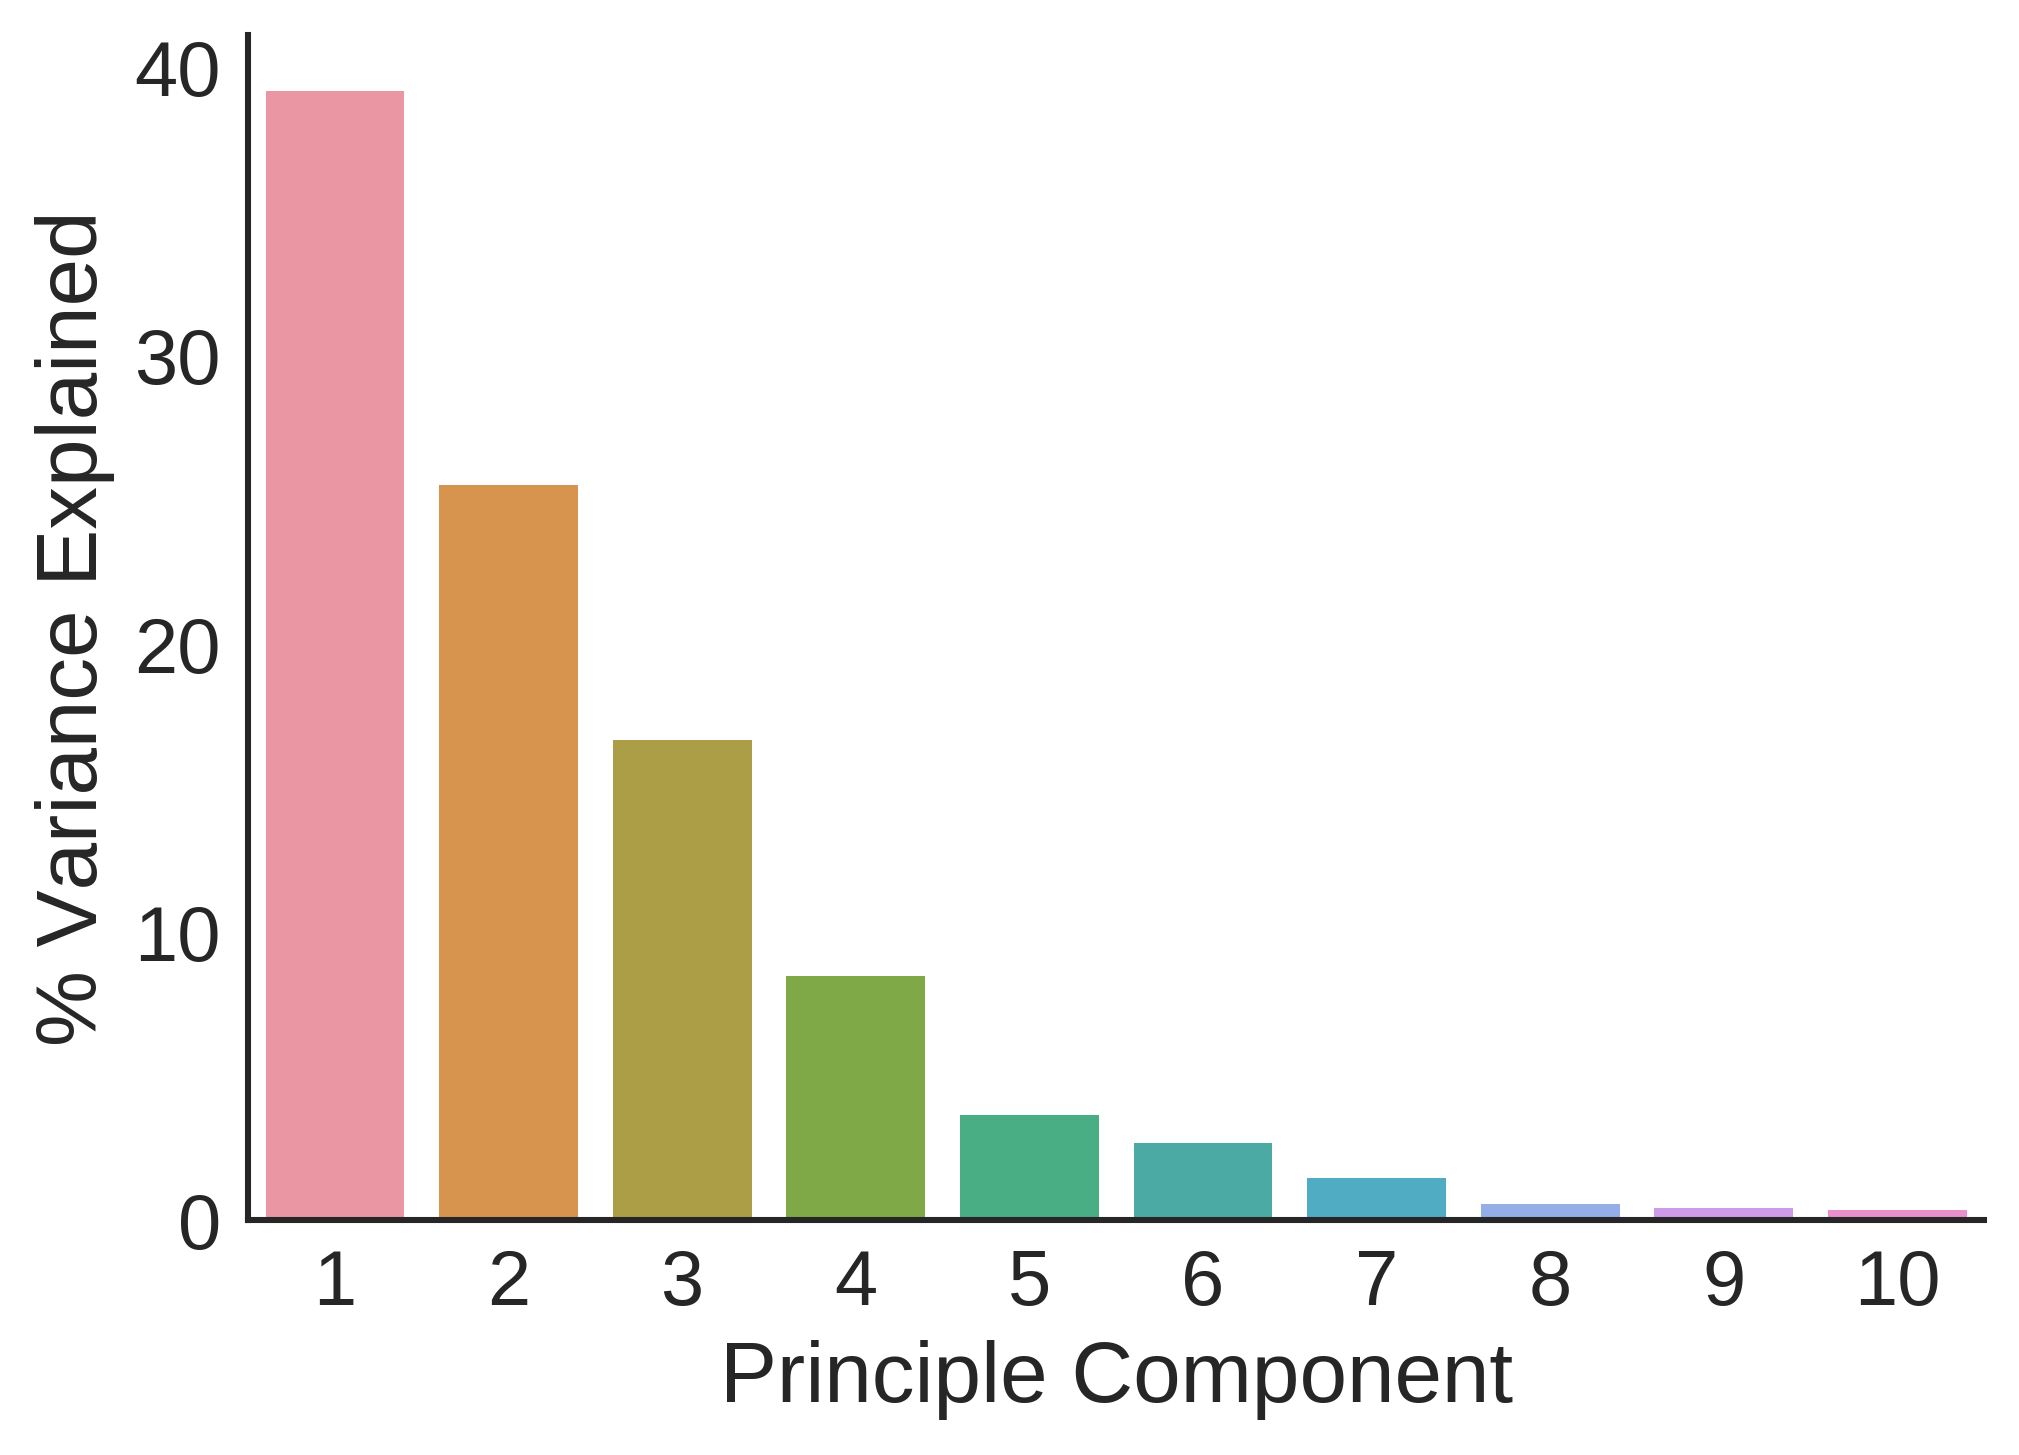
\includegraphics[width=0.8\linewidth]{img/qc/pca_scree}
	\caption{Plot showing the percent of variance explained for the first 10 principal components.}
	\label{fig:qc:scree}
\end{figure}

\begin{figure}
	\centering
	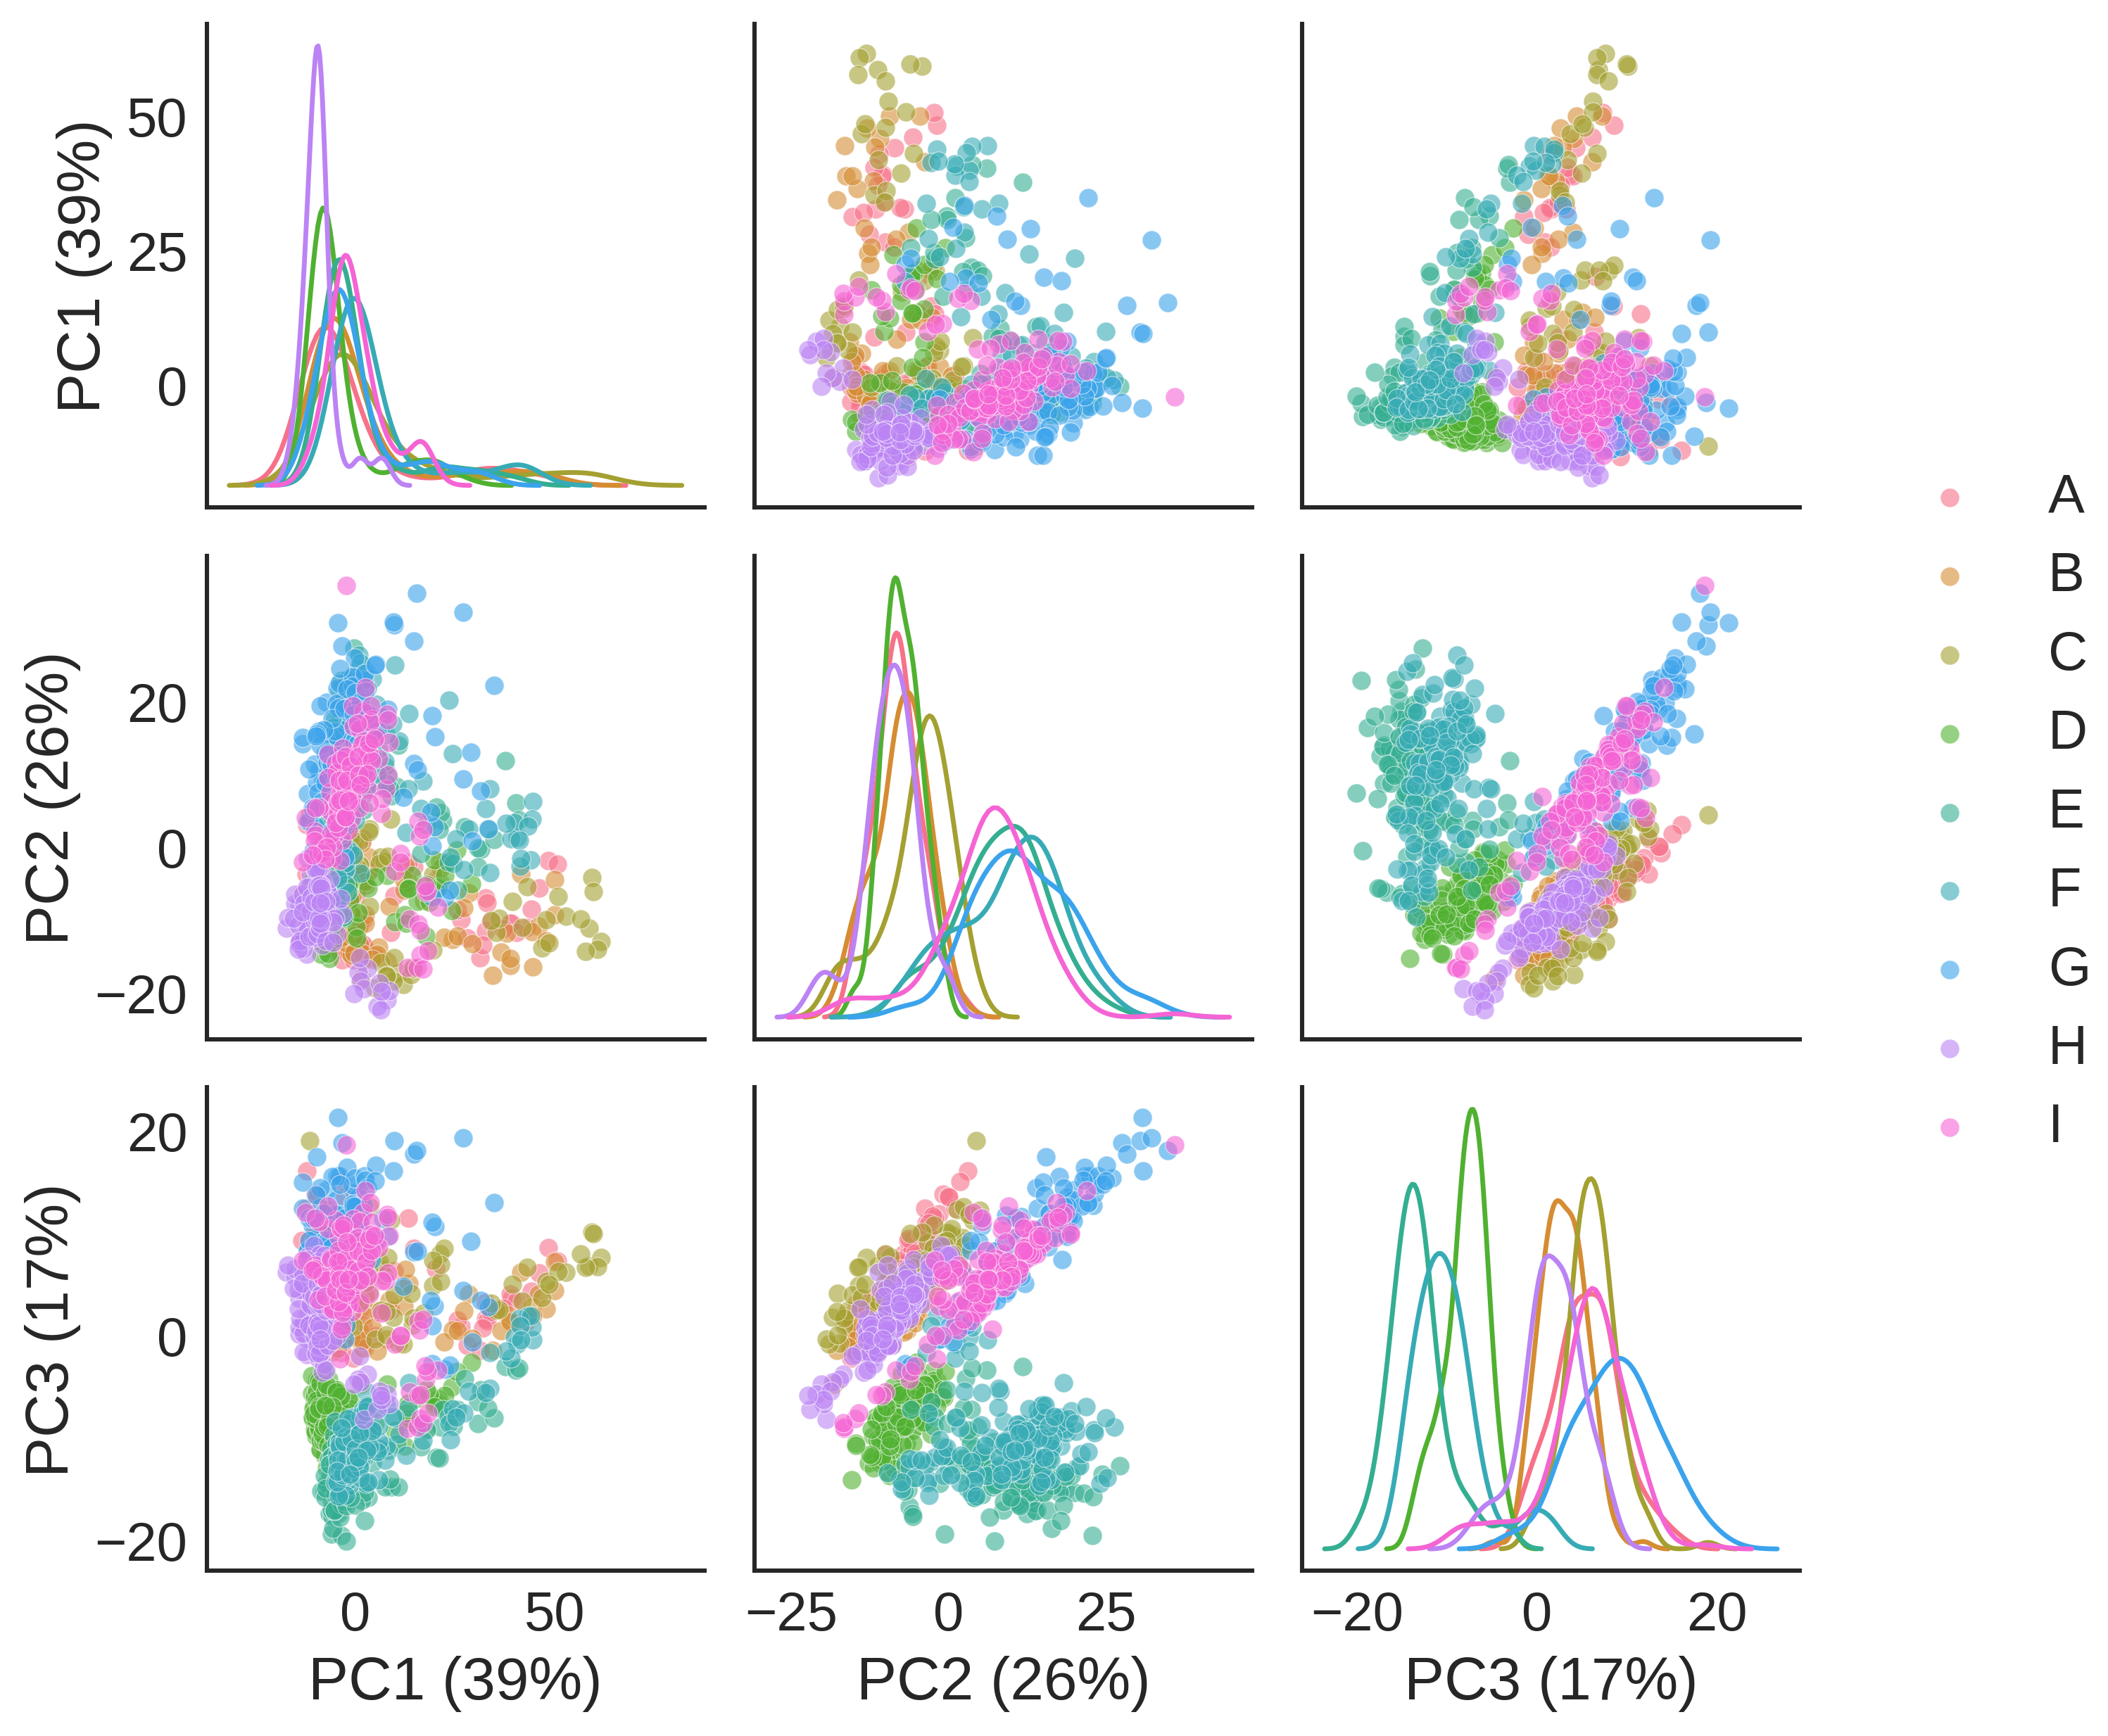
\includegraphics[width=0.8\textwidth]{img/qc/cell_id}
	\caption{Scatter matrix of first three principle components coloured by cell id.}
	\label{fig:qc:cell_id}
\end{figure}

\begin{figure}
	\centering
	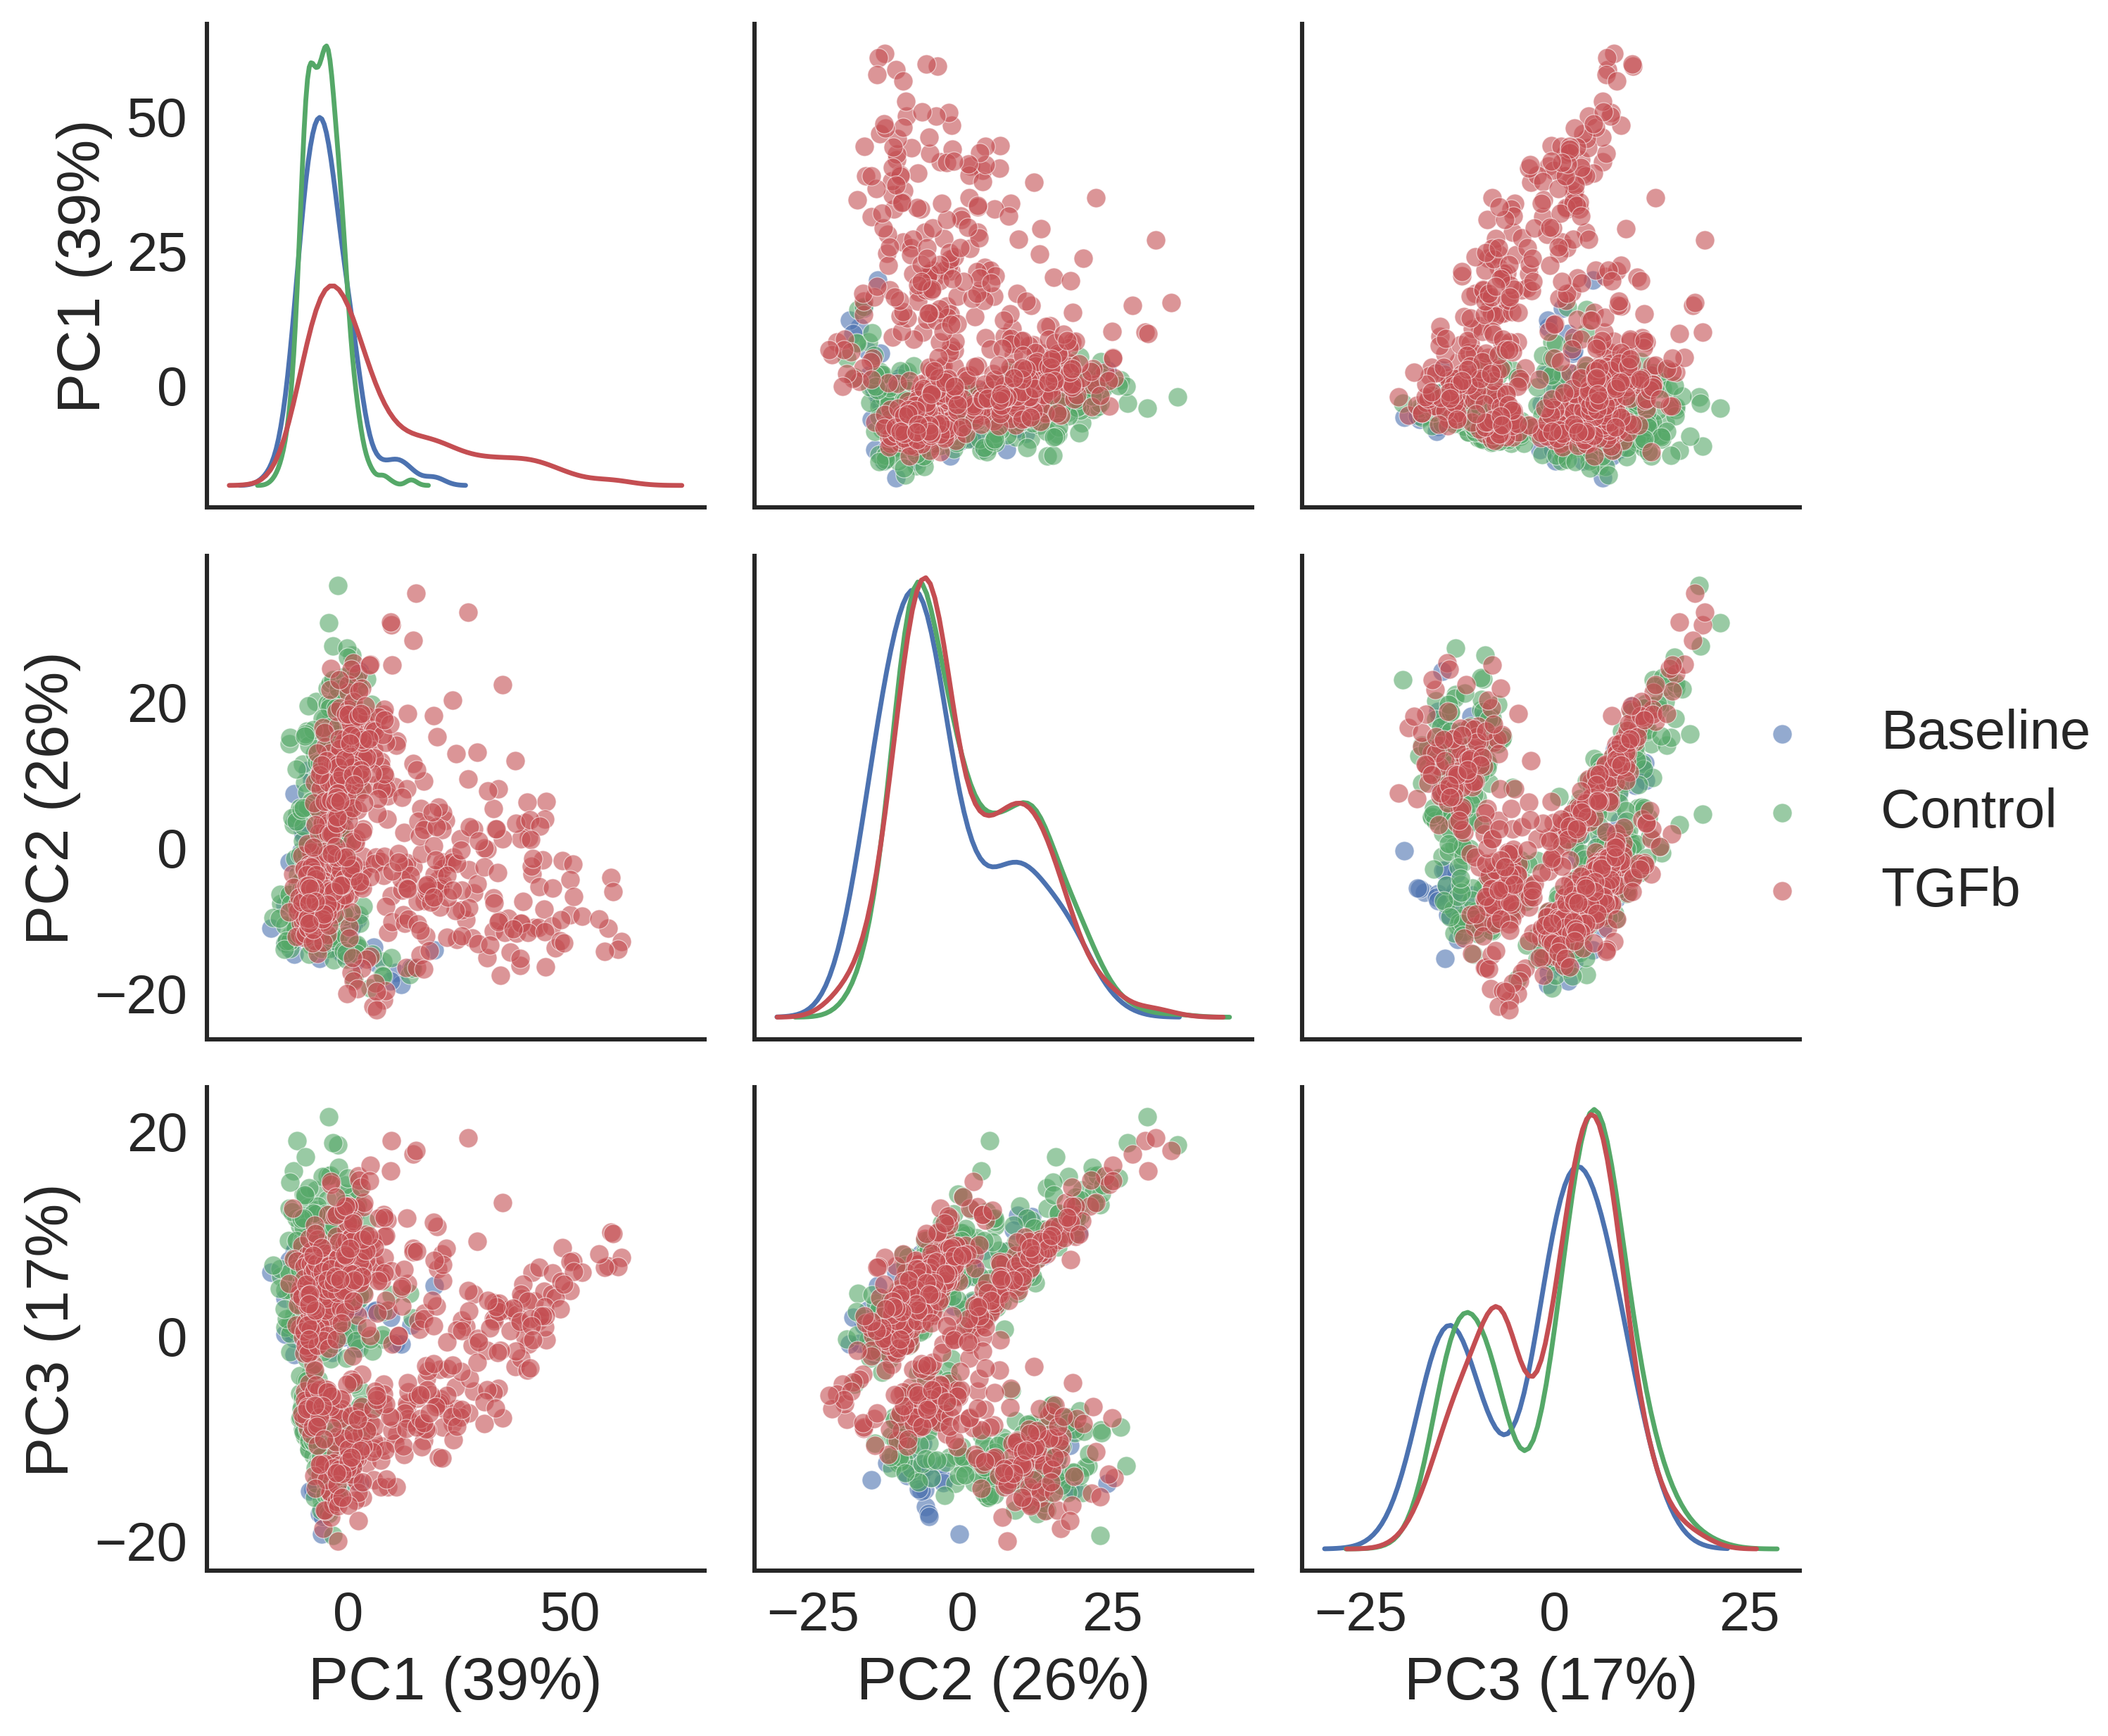
\includegraphics[width=0.8\textwidth]{img/qc/treatment}
	\caption{Scatter matrix of first three principle components coloured by treatment.}
	\label{fig:qc:treatment}
\end{figure}

\begin{figure}
	\centering
	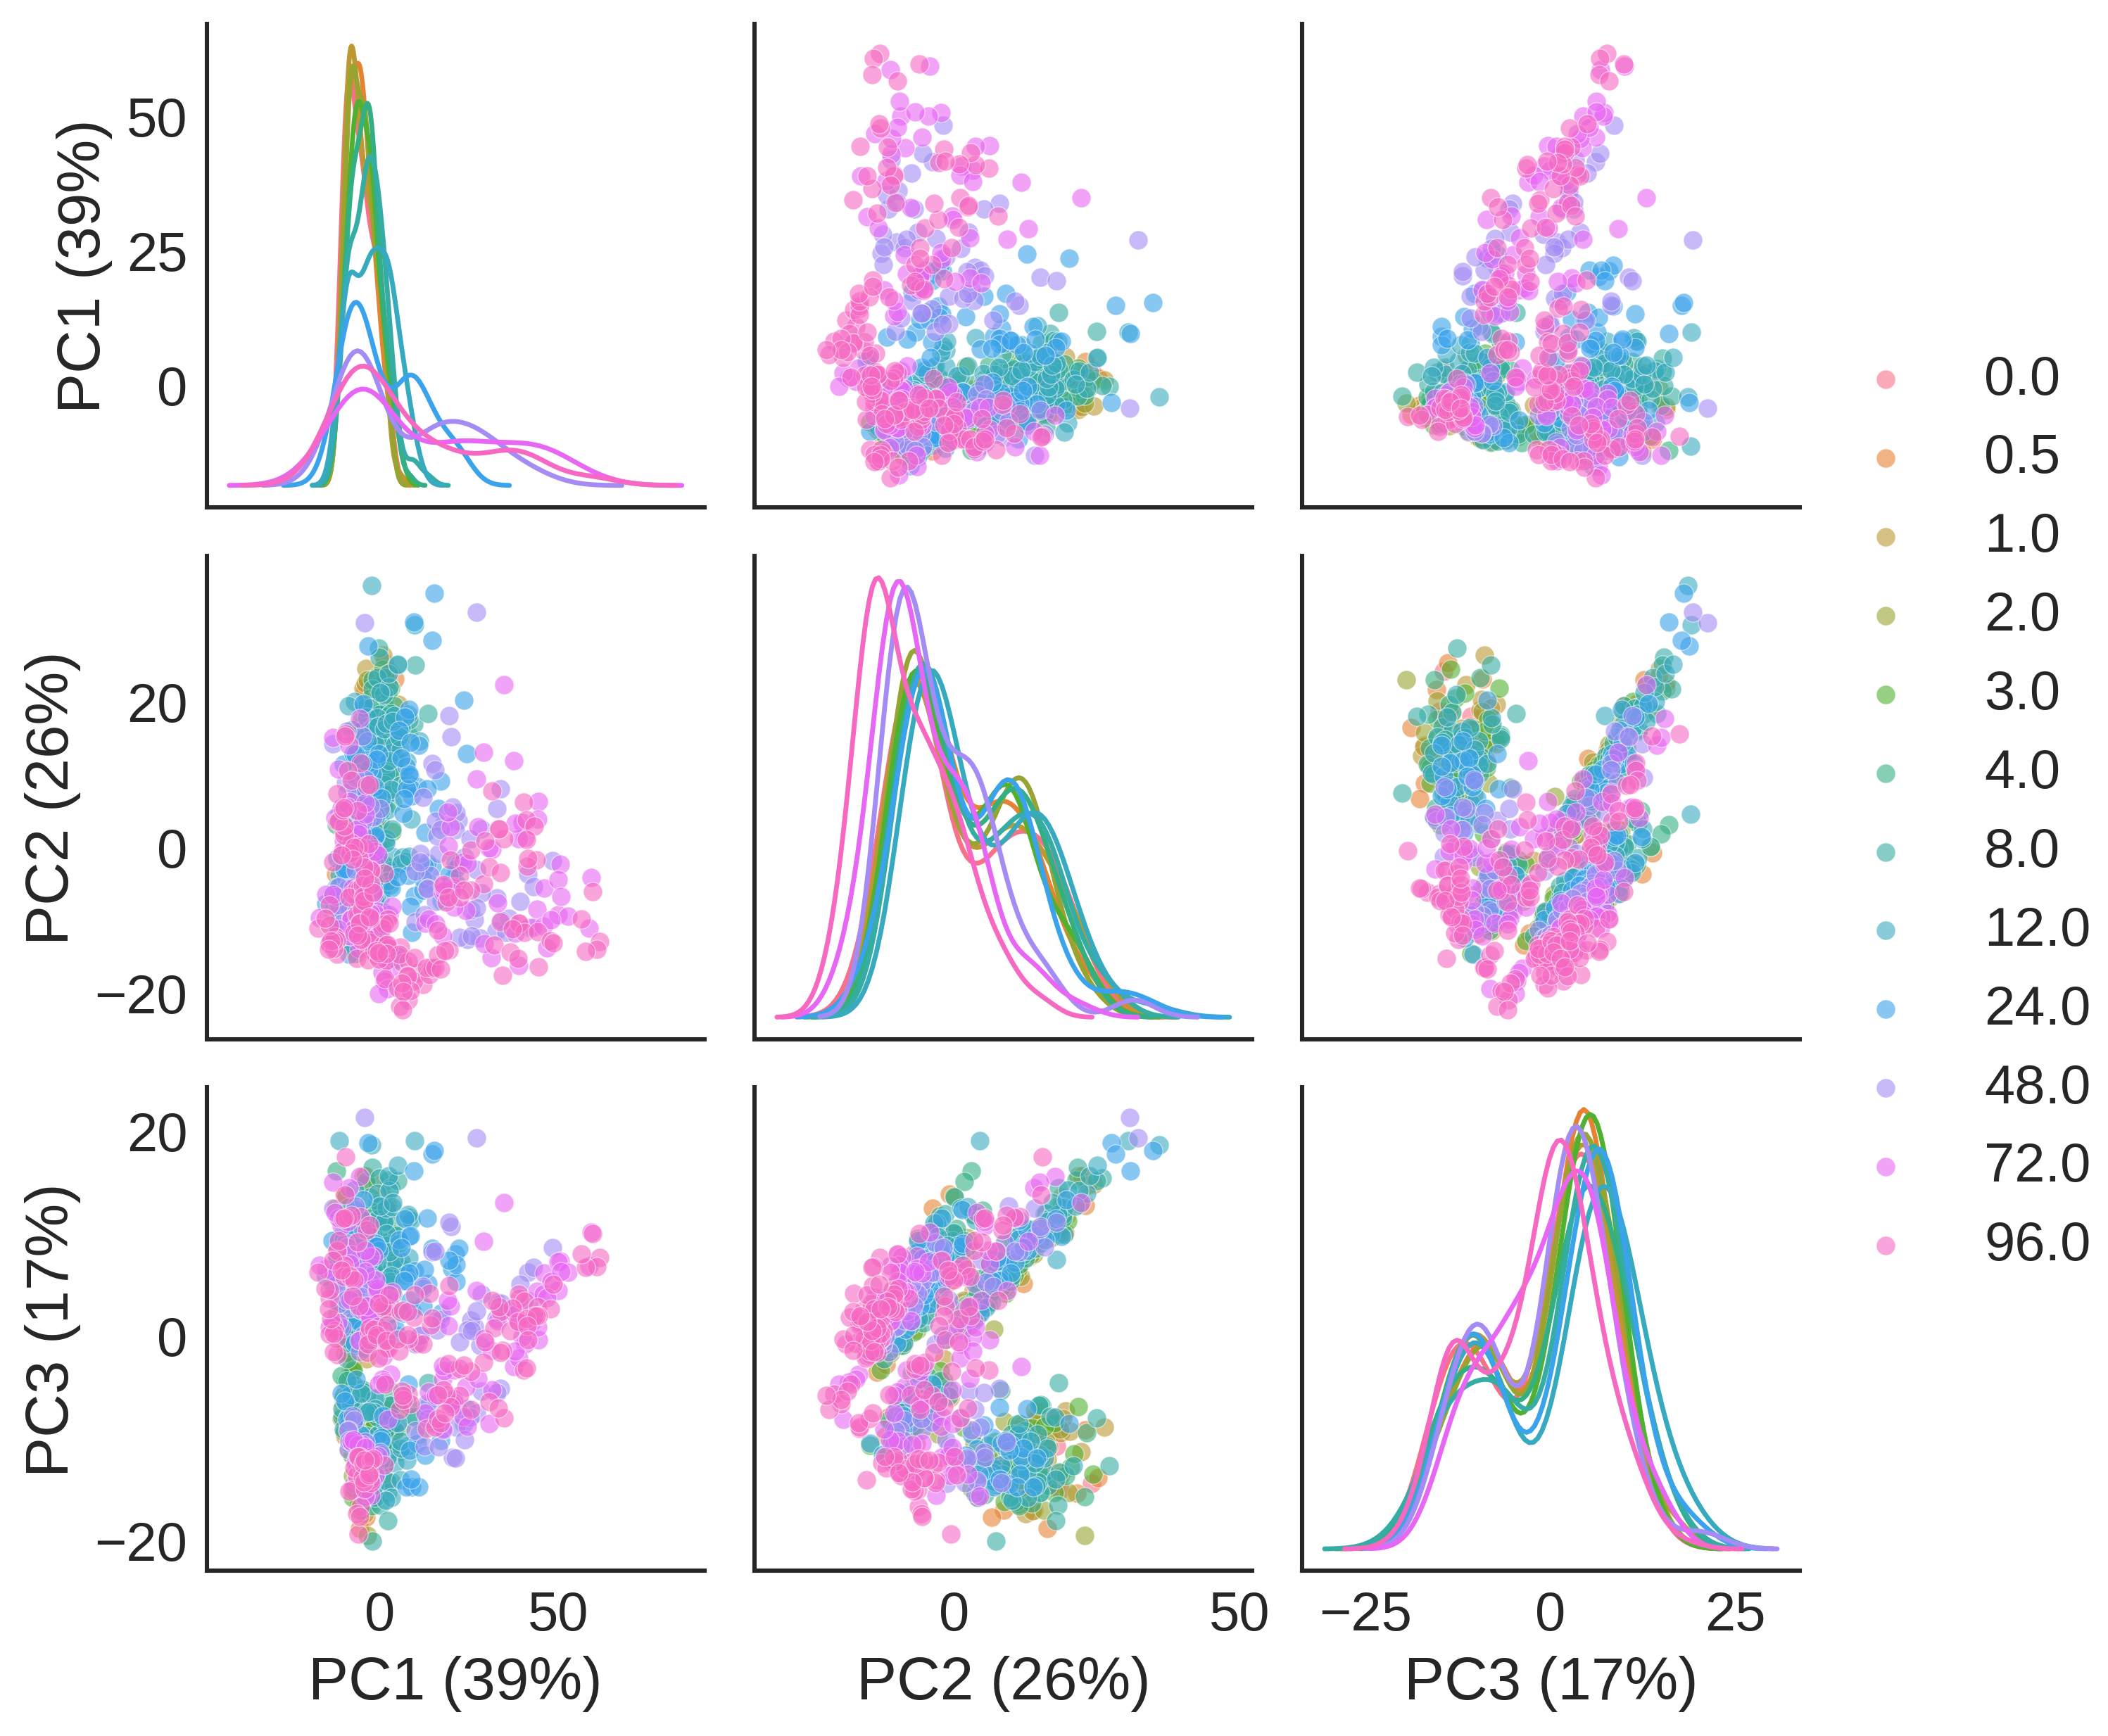
\includegraphics[width=0.8\textwidth]{img/qc/time_point}
	\caption{Scatter matrix of first three principle components coloured by time point.}
	\label{fig:qc:time_point}
\end{figure}

\begin{figure}
	\centering
	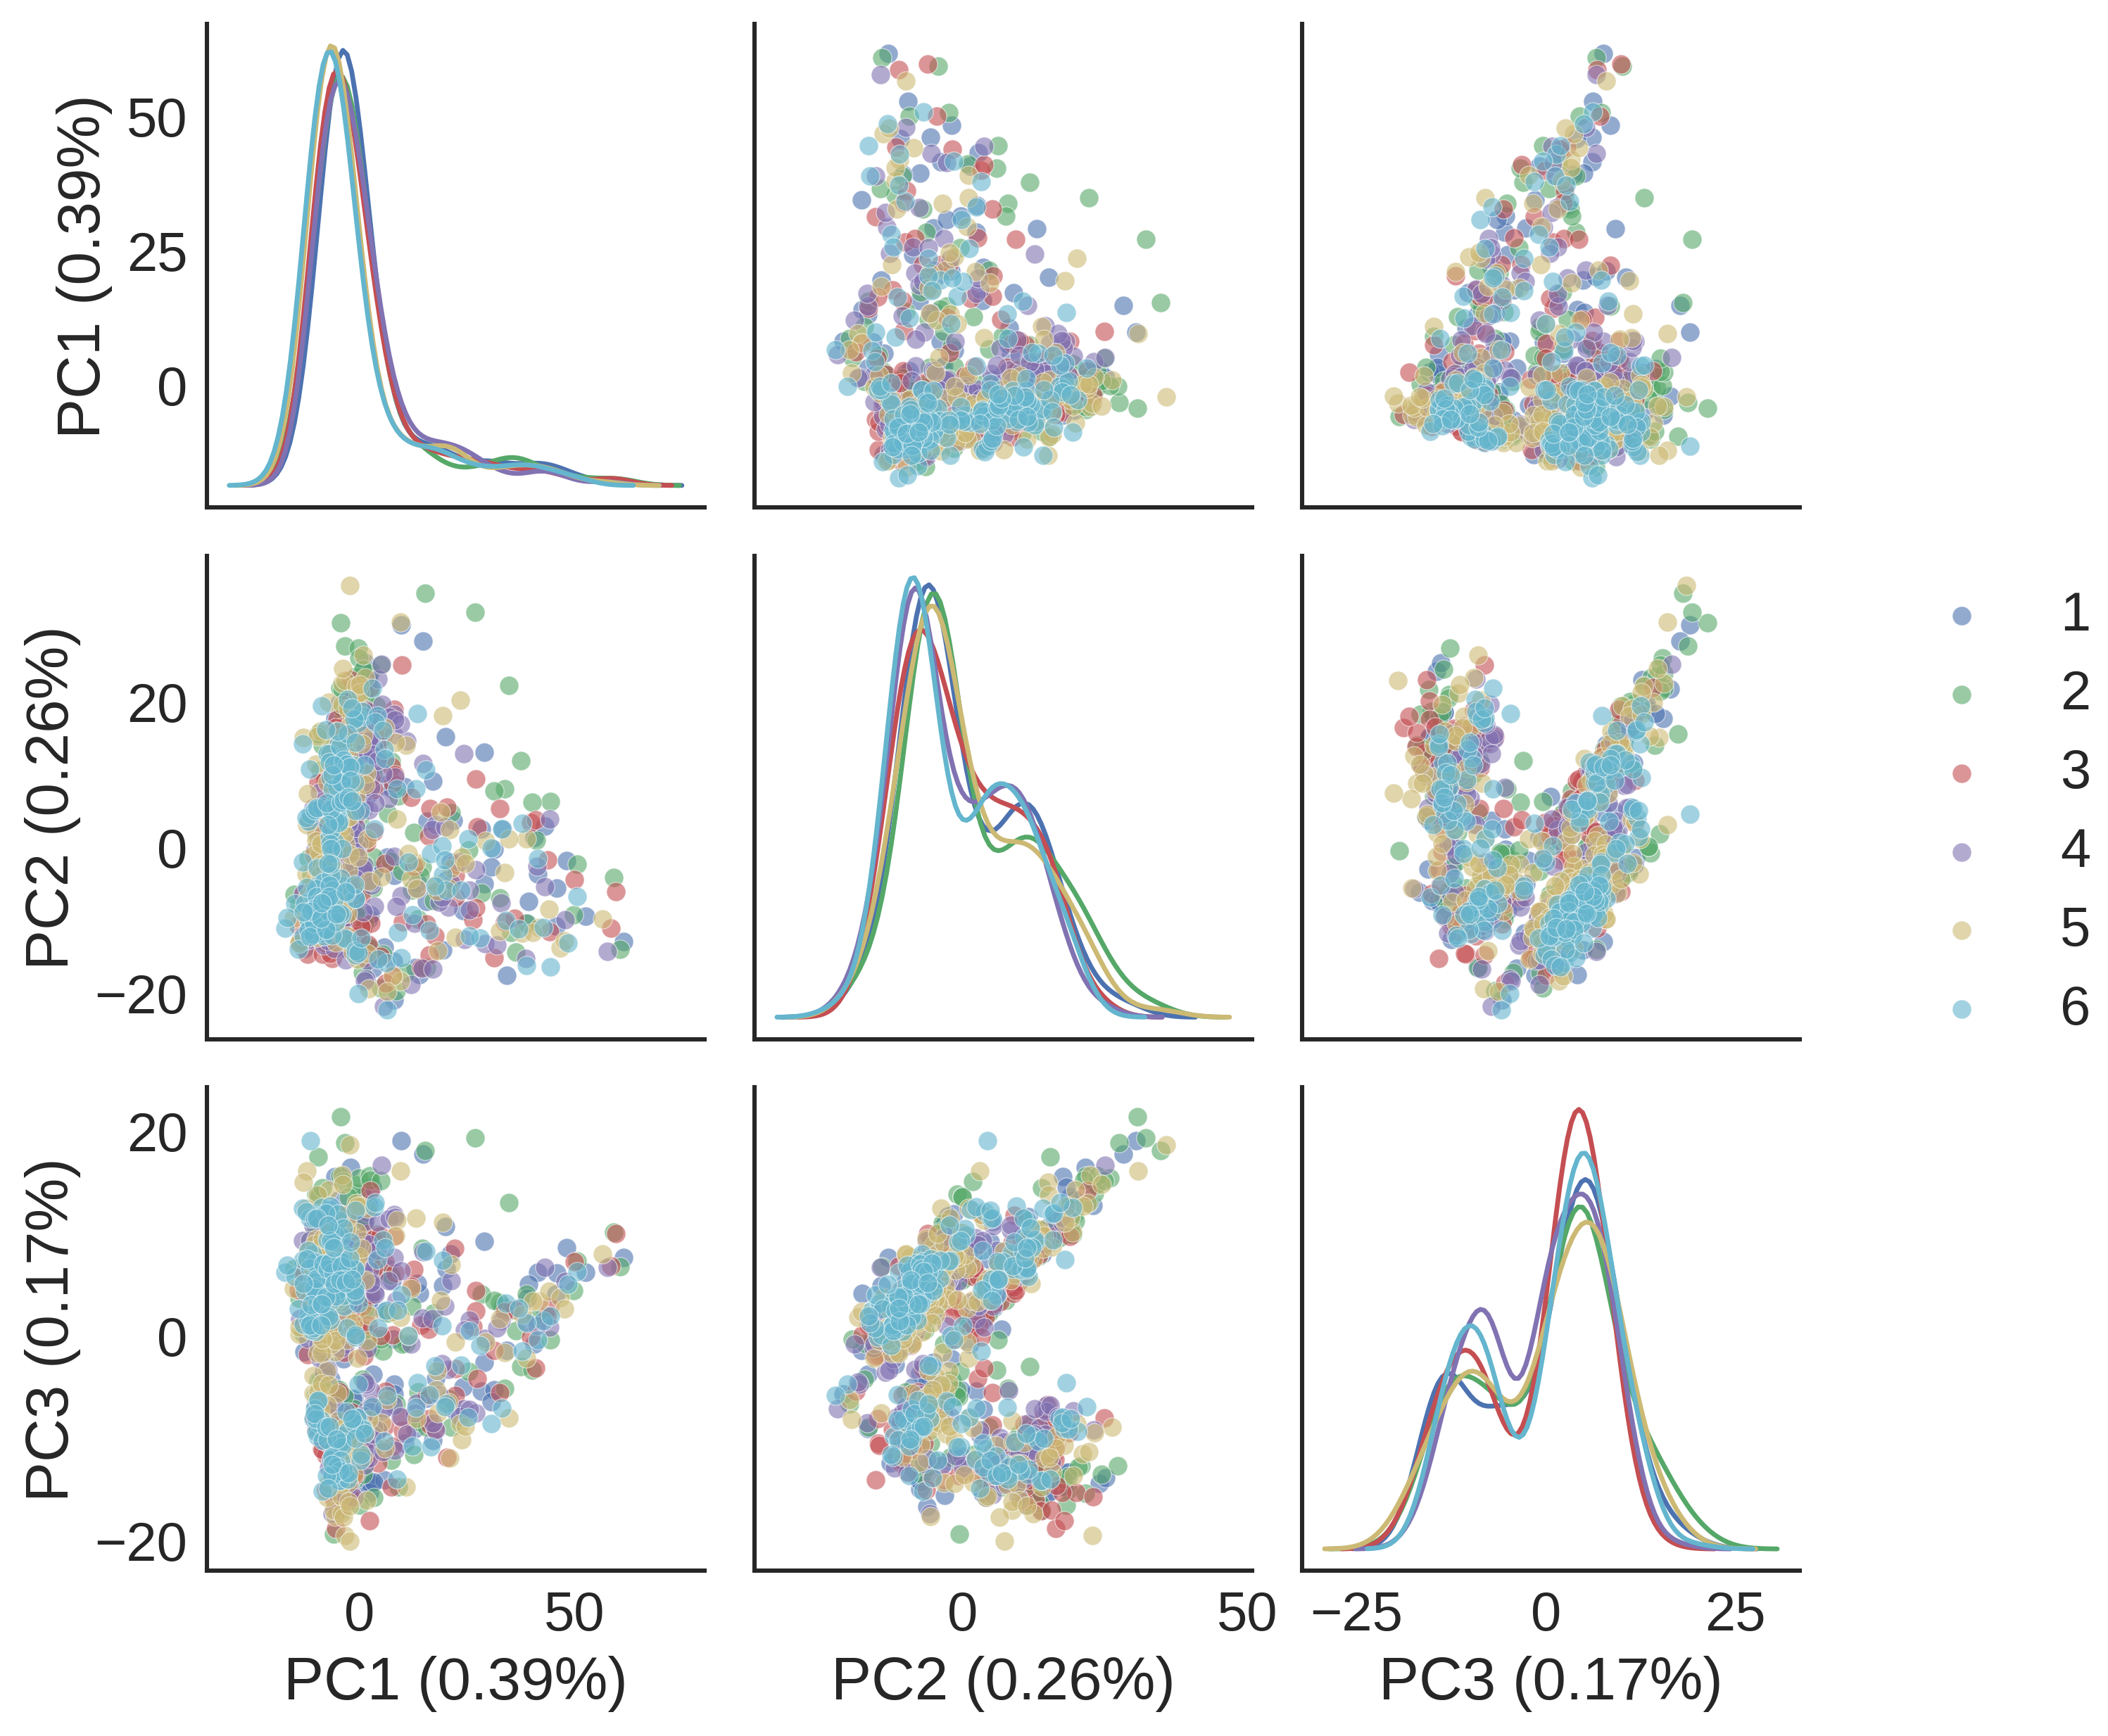
\includegraphics[width=0.8\textwidth]{img/qc/replicate}
	\caption{Scatter matrix of first three principle components coloured by replicate.}
	\label{fig:qc:replicate}
\end{figure}

\end{document}

%%%%Extras
%
%
%%
%%Given the wide spread actions of \tgf{} in ECM biology, \tgf{} has been the focus of some research into the ageing dermis. For instance, \cite{Quan2010} measured reduced levels of \tgf{}1, connective tissue growth factor (CTGF) and type 1 collagen mRNA and protein levels in aged compared to young dermis. 
%%
%%TGFb stimulates CTGF which facilitates ECM production \citep{Quan2010}
%%- CTGF, COL1A1 and TGF are all down regulated in age. 
%%
%%\citep{Quan2015} cited \cite{Quan2010} for showing that \tgf{} controls collagen degradation. However, \cite{Quan2010} does not show this. 
%%
%%
%%What causes the change in ECM composition? To answer, we first must ask: "what are the differences?".
%%
%%the aged dermal phenotype is inferior to a young dermis in terms of ability to perform its functions. 
%%
%%
%%
%%A critical step in determing the causes of the differences between young and old dermis is identifying where the differences exist. 
%%
%%
%%The aged phenotype contains collagen and elastin networks which are impaired both by reduced production and enhanced degradation \citep{Variani2006}.
%%
%%
%%
%%  
%%
%%With age, both collagen and elastin networks become damaged and fewer in number, particularly in photoexposed regions . Accumulation of damaged ECM results in loss of strength and elasticity of the ECM and disorganisation of ECM components. Elastin fibres that are single stranded in young dermis become beaded and loose connectivity with the epidermis in age \citep{Seite2006}. High levels of degradation coupled with reduced replenishment from fibroblasts result in loss of collagen density and integrity \citep{Quan2002, Quan2009, Quan2013}.
%%
%%
%%
%%The dermis is vital for skin integrity and provides structural and nourishing support roles for the avascular epidermis. The dermis is essentially a complex fibrillar mesh of collagens, elastins, glycoproteins and proteoglycans \citep{Lu2011}. Type I collagen is the major constituent of the dermal extracellular matrix (ECM) comprising approximately 80\% of total dermal collagens. The remaining 20\% is composed mostly of type III collagens together with elastins and other proteins which are specialised for performing dermal function.
%%
%%
%%
%% The properties of skin such as its elasticity and strength result from the complex mixture of proteins
%%
%%The skin is composed of a complex set of layers which together provide 
%
%%Structurally, skin is composed of the epidermal, dermal and hypodermal compartments with a complex array of skin appendages such as hair follicles and exocrine glands. Like other tissues, the structure of skin is progressively altered with age. Epidermal-dermal interdigitations flatten, reducing the surface area for adhesion and reduce the strength of the bond between these two tissues. Both epidermal and dermal compartments become thinner with age and the dermal-epidermal junction becomes disorganised and less able to facilitate communication between the two tissues \citep{Farage2009}. 
%
%%The dermis is vital for skin integrity and provides structural and nourishing support roles for the avascular epidermis. The dermis is essentially a complex fibrillar mesh of collagens, elastins, glycoproteins and proteoglycans \citep{Lu2011}. Type I collagen is the major constituent of the dermal extracellular matrix (ECM) comprising approximately 80\% of total dermal collagens. The remaining 20\% is composed mostly of type III collagens together with elastins and other proteins which are specialised for performing dermal function.
%
%%Dermal fibroblasts are the resident caretakers of the dermis: they synthesize, secrete and assemble the dermal ECM as well as matrix metalloproteinases (MMPs) which degrade it (\cite{Varga1987}, (another ref for MMPs)). With age, both collagen and elastin networks become damaged and fewer in number, particularly in photoexposed regions \citep{Variani2006}. Accumulation of damaged ECM results in loss of strength and elasticity of the ECM and disorganisation of ECM components. Elastin fibres that are single stranded in young dermis become beaded and loose connectivity with the epidermis in age \citep{Seite2006}. High levels of degradation coupled with reduced replenishment from fibroblasts result in loss of collagen density and integrity \citep{Quan2002, Quan2009, Quan2013}.
%
%%In young skin, fibroblasts adhere to the ECM by focal adhesions, which create mechanical tension within the fibroblast and creates its stretched out morphology. In age, reduced levels of collagens and other ECM proteins combined with the increased prevalence of collagen fragmentation, reduces fibroblasts ability to adhere to the ECM, causing a lack of mechanical tension and a globular fibroblast morphology with little cytoplasm. Fibroblasts with a globular morphology are less able to perform their function as dermal caretakers, which in turn results in the accumulation of more damage and a positive feedback loop \citep{Quan2015, Cole2018}. 
%
%%The prevalence of senescent fibroblasts with age  	
%
%
%%Fibrobalsts -> role in dermis. senscene ce
%%
%%Exascerbating the problem are the prelevance of senscent fibrobaslts
%
%%%% Instructions from MSB
%%The Introduction should be succinct and provide only the necessary
%%background information, rather than a comprehensive review of the
%%specific field. It should not contain subheadings.

